%%%%%%%%%%%%%%%%%%%%%%%%%%%%%%%%%%%%%%%%%
% Masters/Doctoral Thesis 
% LaTeX Template
% Version 2.5 (27/8/17)
%
% This template was downloaded from:
% http://www.LaTeXTemplates.com
%
% Version 2.x major modifications by:
% Vel (vel@latextemplates.com)
%
% This template is based on a template by:
% Steve Gunn (http://users.ecs.soton.ac.uk/srg/softwaretools/document/templates/)
% Sunil Patel (http://www.sunilpatel.co.uk/thesis-template/)
%
% Template license:
% CC BY-NC-SA 3.0 (http://creativecommons.org/licenses/by-nc-sa/3.0/)
%
%%%%%%%%%%%%%%%%%%%%%%%%%%%%%%%%%%%%%%%%%

%----------------------------------------------------------------------------------------
%	PACKAGES AND OTHER DOCUMENT CONFIGURATIONS
%----------------------------------------------------------------------------------------

% https://tex.stackexchange.com/q/537928/142924
\RequirePackage{yax}
\let\texapiletcs\letcs
\let\letcs\relax
\RequirePackage{etoolbox}
\let\etoolboxletcs\letcs

\documentclass[
11pt, % The default document font size, options: 10pt, 11pt, 12pt
%oneside, % Two side (alternating margins) for binding by default, uncomment to switch to one side
english, % ngerman for German
singlespacing, % Single line spacing, alternatives: onehalfspacing or doublespacing
%draft, % Uncomment to enable draft mode (no pictures, no links, overfull hboxes indicated)
%nolistspacing, % If the document is onehalfspacing or doublespacing, uncomment this to set spacing in lists to single
%liststotoc, % Uncomment to add the list of figures/tables/etc to the table of contents
%toctotoc, % Uncomment to add the main table of contents to the table of contents
%parskip, % Uncomment to add space between paragraphs
%nohyperref, % Uncomment to not load the hyperref package
headsepline, % Uncomment to get a line under the header
%chapterinoneline, % Uncomment to place the chapter title next to the number on one line
%consistentlayout, % Uncomment to change the layout of the declaration, abstract and acknowledgements pages to match the default layout
]{MastersDoctoralThesis} % The class file specifying the document structure

\usepackage[utf8]{inputenc} % Required for inputting international characters
\usepackage[T1]{fontenc} % Output font encoding for international characters
\usepackage{mathpazo} % Use the Palatino font by default
\usepackage[backend=bibtex,style=numeric,natbib=true]{biblatex}
% was: backend=bibtex,style=authoryear,natbib=true
% Use the bibtex backend with the authoryear citation style (which resembles APA)

\addbibresource{references.bib} % The filename of the bibliography

\usepackage[autostyle=true]{csquotes} % Required to generate language-dependent quotes in the bibliography

%%%% added by me %%%%
\usepackage{bookmark}
\usepackage{todonotes}
\usepackage[cmex10]{amsmath}
\usepackage{graphicx}
\usepackage{subcaption}
\usepackage{stfloats}
\usepackage{eurosym}
\usepackage{multirow}
\usepackage{tabu}
% for SmartCheck
\usepackage{colortbl}
\usepackage{booktabs}
\usepackage{graphicx}
\usepackage{multirow}
\usepackage{pgfplots}
\usepackage{pgfplotstable}
\usepackage{tikz}
\usepackage{tikz-qtree}
\usepackage{xcolor}
\usepackage{listings}

\usepackage{mathtools}
\usepackage[noabbrev, capitalize]{cleveref}

\usepackage{syntax}
\usepackage{algorithm2e}

\usepackage{epigraph}

%\usepackage{underscore}
\usepackage{hyperref} % as per its manual, must be added last


% for Findel, KYC
% https://tex.stackexchange.com/a/61266/142924
\newtheorem{definition}{Definition}
\newcommand{\missing}[1]{\textcolor{red}{#1}}
\newcommand*\rot{\rotatebox{90}}

\graphicspath{{Chapters/Chapter03/figures/}{Chapters/Chapter04/figures/}{Chapters/Chapter06/figures/}{Chapters/Chapter07/figures/}{Chapters/Chapter12/figures/}}

\setcounter{secnumdepth}{3} % for references to subsubsections in SmartCheck
% use \subsubsection* to avoid 4-digit numbering elsewhere
%\setcounter{tocdepth}{2}	% but don't include subsubsections in ToC
\setcounter{tocdepth}{3}	% include subsubsections in ToC


%----------------------------------------------------------------------------------------
%	MARGIN SETTINGS
%----------------------------------------------------------------------------------------

\geometry{
	paper=a4paper, % Change to letterpaper for US letter
	inner=2.5cm, % Inner margin
	outer=3.8cm, % Outer margin
	bindingoffset=.5cm, % Binding offset
	top=1.5cm, % Top margin
	bottom=1.5cm, % Bottom margin
	%showframe, % Uncomment to show how the type block is set on the page
}

%----------------------------------------------------------------------------------------
%	THESIS INFORMATION
%----------------------------------------------------------------------------------------

\thesistitle{Security and Privacy of Blockchain Protocols and Applications} % Your thesis title, this is used in the title and abstract, print it elsewhere with \ttitle
\supervisor{Dr. Alex \textsc{Biryukov}} % Your supervisor's name, this is used in the title page, print it elsewhere with \supname
\examiner{} % Your examiner's name, this is not currently used anywhere in the template, print it elsewhere with \examname
\degree{Doctor of Philosophy} % Your degree name, this is used in the title page and abstract, print it elsewhere with \degreename
\author{Sergei \textsc{Tikhomirov}} % Your name, this is used in the title page and abstract, print it elsewhere with \authorname
\addresses{} % Your address, this is not currently used anywhere in the template, print it elsewhere with \addressname

\subject{Computer Science} % Your subject area, this is not currently used anywhere in the template, print it elsewhere with \subjectname
\keywords{} % Keywords for your thesis, this is not currently used anywhere in the template, print it elsewhere with \keywordnames
\university{\href{https://wwwen.uni.lu/}{University of Luxembourg}} % Your university's name and URL, this is used in the title page and abstract, print it elsewhere with \univname
\department{\href{https://wwwen.uni.lu/research/fstm/dcs}{Department of Computer Science}} % Your department's name and URL, this is used in the title page and abstract, print it elsewhere with \deptname
\group{\href{https://www.cryptolux.org/}{CryptoLUX Research Group}} % Your research group's name and URL, this is used in the title page, print it elsewhere with \groupname
\faculty{\href{https://wwwen.uni.lu/fstm}{Faculty of Science, Technology and Medicine}} % Your faculty's name and URL, this is used in the title page and abstract, print it elsewhere with \facname

\AtBeginDocument{
\hypersetup{pdftitle=\ttitle} % Set the PDF's title to your title
\hypersetup{pdfauthor=\authorname} % Set the PDF's author to your name
\hypersetup{pdfkeywords=\keywordnames} % Set the PDF's keywords to your keywords
}

\begin{document}

\frontmatter % Use roman page numbering style (i, ii, iii, iv...) for the pre-content pages

\pagestyle{plain} % Default to the plain heading style until the thesis style is called for the body content

%----------------------------------------------------------------------------------------
%	TITLE PAGE
%----------------------------------------------------------------------------------------

\begin{titlepage}
\begin{center}

\vspace*{.06\textheight}
{\scshape\LARGE \univname\par}\vspace{1.5cm} % University name
\textsc{\Large Doctoral Thesis}\\[0.5cm] % Thesis type

\HRule \\[0.4cm] % Horizontal line
{\huge \bfseries \ttitle\par}\vspace{0.4cm} % Thesis title
\HRule \\[1.5cm] % Horizontal line
 
\begin{minipage}[t]{0.4\textwidth}
\begin{flushleft} \large
\emph{Author:}\\
\href{https://s-tikhomirov.github.io/about/}{\authorname} % Author name - remove the \href bracket to remove the link
\end{flushleft}
\end{minipage}
\begin{minipage}[t]{0.4\textwidth}
\begin{flushright} \large
\emph{Supervisor:} \\
\href{https://www.cryptolux.org/index.php/Alex\_Biryukov}{\supname} % Supervisor name - remove the \href bracket to remove the link  
\end{flushright}
\end{minipage}\\[3cm]
 
\vfill

\large \textit{A thesis submitted in fulfillment of the requirements\\ for the degree of \degreename}\\[0.3cm] % University requirement text
\textit{in the}\\[0.4cm]
\groupname\\\deptname\\[2cm] % Research group name and department name
 
\vfill

{\large \today}\\[4cm] % Date
%\includegraphics{Logo} % University/department logo - uncomment to place it
 
\vfill
\end{center}
\end{titlepage}

%----------------------------------------------------------------------------------------
%	DECLARATION PAGE
%----------------------------------------------------------------------------------------
\iffalse % not seen in other theses in our group
\begin{declaration}
\addchaptertocentry{\authorshipname} % Add the declaration to the table of contents
\noindent I, \authorname, declare that this thesis titled, \enquote{\ttitle} and the work presented in it are my own. I confirm that:

\begin{itemize} 
\item This work was done wholly or mainly while in candidature for a research degree at this University.
\item Where any part of this thesis has previously been submitted for a degree or any other qualification at this University or any other institution, this has been clearly stated.
\item Where I have consulted the published work of others, this is always clearly attributed.
\item Where I have quoted from the work of others, the source is always given. With the exception of such quotations, this thesis is entirely my own work.
\item I have acknowledged all main sources of help.
\item Where the thesis is based on work done by myself jointly with others, I have made clear exactly what was done by others and what I have contributed myself.\\
\end{itemize}
 
\noindent Signed:\\
\rule[0.5em]{25em}{0.5pt} % This prints a line for the signature
 
\noindent Date:\\
\rule[0.5em]{25em}{0.5pt} % This prints a line to write the date
\end{declaration}
\fi

\cleardoublepage

%----------------------------------------------------------------------------------------
%	QUOTATION PAGE
%----------------------------------------------------------------------------------------

\vspace*{0.2\textheight}

\noindent\enquote{\itshape 
	Imagine there was a base metal as scarce as gold but with the following properties:
	
	- boring grey in colour
	
	- not a good conductor of electricity
	
	- not particularly strong, but not ductile or easily malleable either
	
	- not useful for any practical or ornamental purpose 
	
	and one special, magical property:
	
	- can be transported over a communications channel.}\bigbreak

\hfill Satoshi Nakamoto
% https://bitcointalk.org/index.php?topic=583.msg11405#msg11405

%----------------------------------------------------------------------------------------
%	ABSTRACT PAGE
%----------------------------------------------------------------------------------------

\begin{abstract}
\addchaptertocentry{\abstractname} % Add the abstract to the table of contents
This thesis explores various questions related to security and privacy of blockchain systems.

Bitcoin~\cite{nakamoto2008bitcoin} has allowed for the first time to transfer digital units of value without any trusted party.
Alternative cryptocurrencies inspired by Bitcoin aim at better addressing the issues of privacy, scalability, and feature set.
In particular, Ethereum introduces smart contracts in a Turing complete language and a stateful virtual machine, greatly expanding the design space of blockchain application, but expanding the attack surface as well.

In Part~\ref{Part1Privacy}, we discuss the networking layer of Bitcoin and related cryptocurrencies.
We introduce an attack on privacy that allows an adversary to correlated transactions issued by the same user.
We test this technique on Bitcoin, as well as on the major privacy focused cryptocurrency.
We provide a separate overview of privacy-related functionality in mobile wallets.

Part~\ref{Part2Lightning} is dedicated to a promising approach at scaling blockchain, namely, off-chain protocols.
We study the Bitcoin's Lightning Network as the most prominent example of this approach.
We measure the potential effects of certain subset of Lightning nodes on privacy of the users.
Finally, we introduce a probing attack that lets an adversary reveal intermediary balances of payment channels it is not a part of -- the information supposed to be private.

Part~\ref{Part3Ethereum} explores Ethereum.
Ethereum's expressive language, Solidity, provides lots of opportunities for developers to write insecure code.
We propose a simpler language based on Solidity, called Findel, to encode financial agreements in a more declarative fashion.
We study the vulnerabilities in real-world Ethereum contracts and present a tool that automates bug detection in Solidity using static analysis.
Finally, we describe a proposal to limit the privacy-damaging effects of existing legal requirements (know-your-customer, or KYC) if a financial service is implemented on top of Ethereum.
	
\end{abstract}

%----------------------------------------------------------------------------------------
%	ACKNOWLEDGEMENTS
%----------------------------------------------------------------------------------------

\begin{acknowledgements}
\addchaptertocentry{\acknowledgementname} % Add the acknowledgements to the table of contents
This work would not be possible without the help and support of many people.
This is an incomplete list of people to whom I would like to express my deepest gratitude:
\begin{itemize}
	\item My advisor, Prof.~Alex~Biryukov, for the opportunity to freely pursue my interests and for the invaluable support and guidance throughout this journey;
	\item the members of my thesis committee, ... for agreeing to serve as jury members;
	\item my coauthors: ..., for 
	\item colleagues
	\item Uni staff, incl administrative
	\item Luxembourg, for excellent research conditions;
	\item Zcash Foundation, for supporting my work with a grant;
	\item my family, especially for encouraging me to pursue my further education abroad;
	\item Satoshi
\end{itemize}
\end{acknowledgements}
% https://github.com/ZcashFoundation/GrantProposals-2017Q4/issues/24

%----------------------------------------------------------------------------------------
%	LIST OF CONTENTS/FIGURES/TABLES PAGES
%----------------------------------------------------------------------------------------

\tableofcontents % Prints the main table of contents

\listoffigures % Prints the list of figures

\listoftables % Prints the list of tables

%----------------------------------------------------------------------------------------
%	ABBREVIATIONS
%----------------------------------------------------------------------------------------

\begin{abbreviations}{ll} % Include a list of abbreviations (a table of two columns)

\textbf{PoW} & Proof of work \\
\textbf{PoS} & Proof of stake \\
\textbf{LN} & Lightning Network \\
\textbf{CPU} & Central processing unit \\
\textbf{GPU} & Graphics processing unit \\
\textbf{FPGA} & Field-programmable gate array \\
\textbf{ASIC} & Application-specific integrated circuit \\
\textbf{P2P} & Peer-to-peer \\

\end{abbreviations}

%----------------------------------------------------------------------------------------
%	PHYSICAL CONSTANTS/OTHER DEFINITIONS
%----------------------------------------------------------------------------------------

%\begin{constants}{lr@{${}={}$}l} % The list of physical constants is a three column table

% The \SI{}{} command is provided by the siunitx package, see its documentation for instructions on how to use it

%Speed of Light & $c_{0}$ & \SI{2.99792458e8}{\meter\per\second} (exact)\\
%Constant Name & $Symbol$ & $Constant Value$ with units\\

%\end{constants}

%----------------------------------------------------------------------------------------
%	SYMBOLS
%----------------------------------------------------------------------------------------

%\begin{symbols}{lll} % Include a list of Symbols (a three column table)

%$a$ & distance & \si{\meter} \\
%$P$ & power & \si{\watt} (\si{\joule\per\second}) \\
%Symbol & Name & Unit \\

%\addlinespace % Gap to separate the Roman symbols from the Greek

%$\omega$ & angular frequency & \si{\radian} \\

%\end{symbols}

%----------------------------------------------------------------------------------------
%	DEDICATION
%----------------------------------------------------------------------------------------

\dedicatory{For/Dedicated to/To my\ldots} 

%----------------------------------------------------------------------------------------
%	THESIS CONTENT - CHAPTERS
%----------------------------------------------------------------------------------------

\mainmatter % Begin numeric (1,2,3...) page numbering

\pagestyle{thesis} % Return the page headers back to the "thesis" style

% Include the chapters of the thesis as separate files from the Chapters folder
% Uncomment the lines as you write the 	chapters

\chapter{Introduction}

\label{Chapter01Introduction}

\epigraph{Governments are good at cutting off the heads of a [\textit{sic}] centrally controlled networks like Napster, but pure P2P networks like Gnutella and Tor seem to be holding their own.}{Satoshi Nakamoto~\cite{Nakamoto2008}}
\epigraph{If you're not breaking the rules, you're doing it wrong.}{Simon Morris~\cite{Morris2018}}


\section{Foreword}

Bitcoin has emerged at the intersection of two secular trends.
First, computer networks have enabled nearly-instant global connectivity.
The proliferation of the Internet has had a massive economic and societal impact.
Second, the world has abandoned the gold standard in favor of \textit{fiat} money.
Central banks can arbitrarily inflate the supply of national currencies.
The global financial system has become even more interconnected.

Modern finance relies on trust.
Trusting one's counterparty differs from trusting the financial system.
People are free to choose whom they do business with, and trustworthy organizations prosper.
High counterparty trust lowers transaction costs and leads to prosperity.
The financial system, on the contrary, demands the trust of all economic actors.
This trust concentration puts much power in the administrators' hands.
History has shown that they do not always use it responsibly.
Governments routinely abuse their influence over money, printing their way out of deficits at savers' expense.

Cryptographers have been working on digital payment systems since the 1980s.
However, completely removing a trusted administrator has long seemed unsolvable.
The critical challenge is modeling \textit{scarcity}.
Money must be costly to produce, but copying digital data is cheap.
What prevents a malicious user from spending multiple copies of their digital coin?
The traditional solution implies trusting a bank that keeps track of all coins and prevents fraud.
Is it possible to achieve the same result without trusting any single entity?

Bitcoin provides an alternative.
Announced in~2008 and launched in~2009, it is the first system of its kind.
Based on decades of research in cryptography and distributed systems, it models scarcity without a trusted party.
Bitcoin's security relies on a combination of cryptographic algorithms and economic incentives.
We describe the architecture of Bitcoin in more detail in Section~\ref{sec:Bitcoin}.

Bitcoin has spawned a new field of study at the intersection of computer science and economics.
Thousands of alternative cryptocurrencies are exploring various points in the design space.
This thesis attempts to tackle some of the problems in the field, focusing on privacy and security.

In the remainder of this Chapter, we give a more elaborate introduction to cryptocurrencies.
First, we outline the relevant historical context and describe the architecture of Bitcoin.
Then, we list the challenges it faces and the potential ways to address them.
Finally, we outline our original contributions.


\section{Historical overview}

We now provide a historical overview of the two key areas relevant to the development of cryptocurrencies: the Internet and money.

\subsection{Evolution of the Internet}

Information networks developed rapidly in the second half of the XX~century.
Scientists created the first computer networks in~1960s.
ARPANET, the precursor of the Internet, launched in 1969.
In~1981, it connected more than $200$~computers in US-based research centers.

Early communication networks used circuit switching.
Each pair of hosts used a dedicated connection throughout the session.
Internet protocols use another approach -- packet switching.
The sender splits the message into pieces (packets) that travel through the network independently.
The receiver reconstructs the message from the packets.
The sender re-transmits lost or malformed packets.
Packet switching is less reliable but simpler than circuit switching.
It has proved indispensable in connecting heterogeneous networks into the global Internet.

Early computer networks lacked security.
Protocol designers prioritized simplicity over data confidentiality and integrity.
Early Internet users, mostly academics, were not inclined to harm others.
Perhaps more importantly, no cryptographic algorithms were suited for the Internet.

Cryptography studies methods to control information flows.
For hundreds of years, its primary task was hiding information using \textit{symmetric} encryption.
In a classical setting, Alice wants to send a confidential message (the \textit{plaintext}) to Bob.
She \textit{encrypts} the plaintext using a secret \textit{key} and transfers the resulting \textit{ciphertext} to Bob.
Bob uses the same key to \textit{decrypt} the ciphertext into the original plaintext.
An adversary may intercept the ciphertext but cannot decrypt it without the key.

Note that the parties use the same key.
Key establishment is a weak spot of symmetric encryption.
An adversary who intercepts the key can decrypt all messages.
Before the 1970s, two parties could only establish a shared secret by meeting in person or using a physically protected \textit{secure channel}.
Both options are expensive and scale poorly.

Moreover, authentication also depended on a shared key.
It was impossible to convince the counterparty that the message was authentic without giving them the power to sign messages themselves, which is unacceptable for many Internet use cases.
For instance, a company would have to share the signing key with all readers to convince them of the authenticity of a press release.
It immediately follows that all subsequent messages signed by this key cannot be trusted.

Whitfield Diffie and Martin Hellman solved both problems.
In their breakthrough 1976~paper "New directions in cryptography"~\cite{Diffie1976}, they proposed two novel algorithms.
First, they introduced a \textit{key establishment} protocol over an insecure channel.
This algorithm allows two parties to securely generate a shared secret even if an eavesdropper intercepts all their messages.
Second, they described the first \textit{digital signature} algorithm.
A digital signature allows a sender to prove the authenticity of their messages without sharing the signing key.
A new field of cryptography -- \textit{asymmetric} cryptography -- was born.

Asymmetric cryptography enabled the widespread deployment and commercialization of the Internet.
Users could now establish spontaneous secure connections over insecure channels.
Businesses started adopting the Internet in the 1980s.
This process accelerated in the early 1990s with the invention of the World Wide Web and web browsers with a graphical user interface.
Entrepreneurs started the first Internet companies.
Many startups proved nonviable and went bankrupt in the Dot-com crash of 2000.
Their early enthusiasm, even if unjustified, attracted talent and capital into the nascent industry.
The first two decades of the XXI century saw a rapid expansion of Internet businesses.
A new generation of companies built and scaled novel digital services to billions of users.

Modern Internet businesses heavily rely on \textit{networks effects}.
Any network is valuable because it allows its members to communicate.
Therefore, a new user is more likely to join the social network most of their friends already use.
Network effects allow established companies to diminish competition.
Internet giants gather vast amounts of user data across all their services.
Large-scale data analysis helps them fine-tune their products to attract and retain users more efficiently.
This self-reinforcing loop favors the incumbents and concentrates market power.

As a result, the Internet in~2020 is highly concentrated.
The five US-based Internet giants -- Google, Apple, Facebook, Amazon, and Microsoft (abbreviated as \textit{GAFAM}) -- account for $17.5\%$~of the~S\&P market index~\cite{Levy2020}.
GAFAM plus the China-based Alibaba and Tencent are the most valuable companies in the world by market capitalization.
As digital communication now influences most areas of life, Internet giants play an even larger economic and political role.


\subsubsection*{File-sharing networks}
\label{sec:FileSharingNetworks}

Peer-to-peer file-sharing, which became widespread in the 1990s, foreshadowed cryptocurrencies.
At that time, the Internet was gaining adoption in the developed world.
Increased bandwidth allowed users to distribute large files over the Internet.
P2P file-sharing networks were first to satisfy the demand for fast and convenient content sharing.\footnote{Client-server file-sharing predates P2P file-sharing by at least two decades: the File Transfer Protocol (FTP) was introduced in~1971.}

File-sharing networks and cryptocurrencies share two crucial attributes.
First, networks of both types are driving against the trend towards the centralization of the Internet.
Instead of relying on a centralized service provider, they pool resources from users' computers.
Second, they demonstrate that given sufficient economic incentives, a decentralized network is impossible to shut down.
We explain the differences and similarities between file-sharing and cryptocurrency protocols in Chapter~\ref{Chapter02IntroP2P}.

Napster was the first popular file-sharing network.
It launched in~1999.
The protocol was only partially decentralized.
Users hosted the files, and a central server coordinated the exchange.
Napster quickly attracted millions of users.
Widespread sharing of copyrighted content drew the attention of law enforcement.
The administrators shut down the service in~2001 to comply with a court order.
Napster shows how centralization harms resilience.
Without central coordination, Napster users could not locate the files.
The existence of the central server made it \textit{possible} to shut the network down.

Gnutella, introduced in~2000, took another approach to content addressing.\footnote{See an overview and comparison of Napster and Gnutella in~\cite{Saroiu2003}.}
In Gnutella, users forward queries to all their neighbors.
Each neighbor either replies with the requested content or forwards the query further.
This "flooding" approach has no single point of failure but is inefficient.

Distributed hash tables (DHT) offered a compromise by storing the content \textit{index} in a distributed manner.
This approach proved to be resilient and efficient.
A DHT randomly distributes content among nodes.
A searching node forwards the query to the node "closest" to the required file.
DHT allows for efficient querying and minimal network restructuring when nodes leave or join.
Kademlia~\cite{Maymounkov2002} is a popular DHT implementation.

BitTorrent~\cite{Pouwelse2005}, launched in~2001, is arguably the most successful file-sharing protocol.
It strikes a balance between efficiency and resilience by allowing users to locate files via either specialized websites (\textit{torrent trackers}) or a Kademlia-like DHT.

File-sharing networks demonstrate the importance of economic incentives -- the central tenet of cryptocurrencies.
Users of file-sharing networks download content from other users' computers.
A protocol without an identity system cannot force users to upload content.
What motivates uploaders to provide the files for free?

BitTorrent implements measures against free-riding.
First, downloaders receive file chunks from peers who do not have the full file.
In turn, they upload parts of the file back while waiting for their download to complete.
On top of the protocol-based measures, some torrent trackers also account for how much their users upload and download.
The combination of these measures makes BitTorrent sufficiently reliable but not too difficult to use.
The file-sharing ecosystem has attracted both altruistic~\cite{Rehn2004} and profit-driven~\cite{Rumin2010} content distributors.

In~2010s, file-sharing declined in popularity.
However, it applied intense competitive pressure on the entertainment industry.
Streaming services emerged, offering unlimited access to content for a fixed monthly price.\footnote{BitTorrent usage rose in the late 2010s because of the fragmentation of content among streaming services~\cite{Bode2018}.}

File-sharing demonstrated the resiliency of Internet protocols.
Despite copyright infringement lawsuits against torrent trackers and their users, law enforcement could not fully shut down file-sharing networks.
One may argue that this is impossible in principle.
As long as at least two computers are willing to communicate according to the protocol rules, the network lives on.

Resilience is crucial for cryptocurrencies.
As file-sharing networks opposed a powerful entertainment industry oligopoly,\footnote{For example, three major corporations dominate the music industry: Universal Music Group, Sony Music Entertainment, and Warner Music Group.} cryptocurrencies compete with central banks.
If cryptocurrencies live up to their promise, attempts to shut them down are inevitable.


\subsection{Evolution of money}

Money is a form of language to convey value -- a particular type of information.
For example, it conveys that the payer performed some valuable work in the past and wishes to receive something in return now.
Money separates the labor from enjoying its fruit.
Nothing is a universal store of value, because value is subjective.
A future payee may reject payment for myriads of unpredictable reasons.

Throughout history, people used various types of money.
Some goods make better money than others and do so on longer time frames.
Gold is arguably the longest widely recognized money.
It possesses the essential properties of money: recognizability, divisibility, portability, durability, fungibility, and scarcity.

Gold is burdensome to handle directly.
The growing speed of commerce demanded easier methods of payment, such as \textit{representative money} (gold certificates) and, eventually, \textit{fiat money}, disconnected from physical commodities.

Fiat money is the basis of the modern financial system.
In~1971, the US stopped converting dollars to gold, ending the Bretton Woods global monetary system.
The currency exchange rates are now determined by supply and demand.
Governments and central banks strongly influence the market.
They change interest rates, perform market interventions, and enforce capital controls.

This transition has deprived money of its fundamental property -- trustlessness.
Gold is a \textit{bearer asset}.
It is not anyone's liability.
In contrast, a gold certificate holder must trust the issuer to exchange it to gold, and a holder of fiat money must trust the issuer not to dilute its value with excessive issuance.


\subsubsection*{Network effects in money}

Similar to information networks, money exhibits network effects.
People are likely to demand widely accepted currencies for their work.
The world economy tends to converge onto a single currency.
The US dollar already plays this role to a large extent.
It is the most popular reserve currency and the currency of international trade.
One can argue that without legal restrictions (such as the need to pay taxes in local currencies) the US dollar would dominate the global economy.

The effects of centralization induced by network effects are especially adverse in monetary networks.
For example, censorship has more severe consequences: a frozen bank account causes more problems than a blocked social media account.
The issue is even more concerning if physical cash is unavailable.
In many developed countries, such as Sweden and the Netherlands, banks are phasing out cash to combat money laundering.
Without cash, a person banned from the banking system cannot buy necessities.
Money administrators can also change the rules on short notice.
A recent example is the 2016~demonetization in India.
High-denomination banknotes were declared invalid in an attempt to fight black markets.
This sudden move caused severe economic disruption throughout the world's second-most populous country.

A money network has a unique property: all users value the content that it helps exchange.
Financial administrators may abuse this property and print themselves money -- a privilege that their information network counterparts do not enjoy.
A social network administrator can push their writings into everyone's news feeds or inflate the reported number of views but cannot make people perceive their content as universally valuable.\footnote{For example, as of 2020, "only" $116$~million out of $2.5$~billion users of Facebook follow its creator Mark Zuckerberg.}

Switching monetary systems is hard.
People cannot easily "vote with their feet", especially if the administrators abuse their position.
First, it is not always apparent that abuse takes place.
For instance, moderate money printing can long go unnoticed, slowly diluting savings.
Second, it is hard to coordinate which another system to switch to.
Uncoordinated exodus destroys the benefits of network effects.
Finally, monetary administrators deliberately impede exit with legal action.
Multiple independent centralized payment systems were shut down.
Examples include Liberty~Reserve, Liberty~Dollar, and e-gold~\cite{White2014, Trautman2014}.
Others, such as PayPal, were forced to give up their initial vision and merge with the existing financial system~\cite{Jackson2017}.
This state of affairs inclines rational actors to accept the corrupt status quo.


\subsubsection*{Key challenges for digital currencies}

The first digital cash protocols were proposed in the early 1980s, but nearly three decades passed before the first viable solution -- Bitcoin -- was introduced.
Why did designing a decentralized digital currency take so long?

Digital signatures provide only a part of the solution.
Senders sign transactions to reliably prove their intent to spend their money.
The receiver can verify the signature without relying on any authority.\footnote{Assuming that the receiver knows the sender's public key.}
However, asymmetric cryptography is not sufficient.
Two crucial challenges have been hindering the deployment of digital cash protocols for decades.

\paragraph{Double-spending}

One cannot easily copy a physical object.
A metal coin is either in the sender's or the receiver's hand.
In contrast, one can effortlessly copy digital information.
A malicious user can duplicate their "coin" and spend it twice.
This problem is known as \textit{double-spending}.

Balances must be stored on multiple computers to mitigate centralization risks.
However, it is unclear how to ensure consistency.
If two computers report different balances for the same account, how to agree on the right one?

Voting is a questionable solution in this context.
Without an \textit{identity management} system, an adversary can launch a \textit{Sybil attack} and vote multiple times.
One way to combat Sybils implies maintaining a list of all voters and only allowing each of them to vote once.\footnote{This class of problems is called \textit{Byzantine fault tolerant} consensus.
A prominent protocol of this class is \textit{Practical Byzantine fault tolerance} (PBFT)~\cite{Castro2002}.
Cryptocurrencies such as Ripple~\cite{Chase2018} and Stellar~\cite{Mazieres2014} use BFT-like protocols.}
Nevertheless, contrary to the design goals, a party who controls the voter list becomes the central point of control.
To prevent censorship, the network must allow new users to join unconditionally.

How can a network defend against Sybil attacks while providing free access?


\paragraph{Fair emission}

A digital currency must come into circulation somehow.
Who should get the newly created money?

On the one hand, the system should reward the users who help maintain it.
Transaction processing requires resources.
If no central party allocates these resources, users must provide them.
However, without strong identities, economically rational agents would not contribute.
The system needs economic incentives, or it collapses under the burden of free-riders.

On the other hand, users should perceive the currency distribution as fair.
Otherwise, they will not join.
Unlike the fiat system, no one is forcing them to.
The currency distribution must also be objectively verifiable.
All users should be able to independently check that everyone else follows the rules.

How can a network automatically reward anonymous participants proportionally to their contributions?


\subsubsection*{Early digital currencies}

Let us mention notable pre-Bitcoin proposals of digital currency systems.

David Chaum introduced \textit{ecash}, an anonymous digital cash protocol, in 1982~\cite{Chaum1982} and further enhanced it in~1988~\cite{Chaum1988}.
Ecash users would exchange digital coins issued by a bank.
A receiver would consult the bank to verify that the incoming coins had not been spent.
However, the participants' identities would remain hidden from the bank due to \textit{blind signatures}.
In~1989, Chaum founded a company called Digicash to commercialize his invention.
While gaining some traction in mid-1990s,\footnote{For instance, the Dutch authorities considered using Digicash for road toll payments~\cite{Chaum2019}.} the company declared bankruptcy in~1998.

In~1998, Wei Dai proposed \textit{b-money}~\cite{Dai1998}.
B-money, predating Bitcoin by a decade, was in many ways similar to it.
Users, identified by public keys, would independently maintain a list of all current balances.
Any user would be able to generate coins by performing otherwise useless computations.\footnote{"Anyone can create money by broadcasting the solution to a previously unsolved computational problem. The only conditions are that it must be easy to determine how much computing effort it took to solve the problem and the solution must otherwise have no value, either practical or intellectual."}

A crucial piece of the Bitcoin's puzzle is \textit{proof-of-work} (PoW).
Cynthia Dwork and Moni Naor proposed PoW in~1992 as an anti-spam mechanism~\cite{Dwork1992}.
A sender of an electronic message would need to perform computational work.
A \textit{proof} allows anyone to verify the number of computations performed.
The puzzle depends on the message to prevent re-using one solution for different messages or recipients.
PoW would incur a negligible delay for regular users while deferring spammers.

Adam Back suggested using cryptographic hash functions for PoW in his 1997 Hashcash proposal~\cite{Back1997}.
The \textit{work} in Hashcash means finding partial collisions of a cryptographic hash function.
Such functions simulate random oracles.
Thus it is computationally hard to find preimages or partial preimages for them.
One cannot predict whether a function output satisfies a given property without calculating it.
Hence PoW solutions can only be found by trial and error.
Hashcash uses this property as a puzzle with an adjustable level of hardness.

In~2005, Nick Szabo proposed Bitgold~\cite{Szabo2005}.
His idea was to represent digital coins as "a string of bits [computed] from a string of challenge bits."
The solutions to such puzzles would be linked in a chain using multiple timestamping servers to preserve integrity.


\section{Bitcoin}
\label{sec:Bitcoin}

Bitcoin was the first decentralized digital currency to solve the double-spending problem without a trusted third party.
An unknown person under a pseudonym Satoshi Nakamoto announced Bitcoin in October~2008.\footnote{Nakamoto might have deliberately chosen dates with a symbolic meaning while constructing their pseudonymous identity. For instance, Nakamoto claimed to have been born on 5~April~1975. The Executive Order 6102, issued on 5~April~1933, banned private gold ownership in the US\@. The ban was repealed on 31~December~1974. The date for the first public announcement of Bitcoin -- 31~October -- may have also been chosen deliberately. On that day in~1517, Martin Luther nailed his Ninety-five Theses on the door of a church in Wittenberg, starting the European Reformation. It has been argued that Bitcoin may lead to similarly wide-reaching societal shifts~\cite{Demeester2019}.}
Shortly after, he published the source code.
The original code repository was later renamed to \textit{Bitcoin~Core} -- the Bitcoin's \textit{reference implementation}.
Bitcoin launched on 3~January~2009 and started slowly gaining traction in the technology community.

Nakamoto's insight was in the way he combined Bitcoin's components.
All the necessary ingredients had already been proposed, but never connected in the right way.


\subsection{Bitcoin architecture}

Let us now briefly describe the architecture of Bitcoin.
We refer the reader to~\cite{Narayanan2017} for a historical review of Bitcoin's building blocks, to~\cite{Bonneau2015} and~\cite{Tschorsch2016} for an overview of the field, and to~\cite{Narayanan2016} and~\cite{Antonopoulos2014} for a comprehensive technical introduction.

\paragraph{Nodes and P2P network}

The Bitcoin network consists of \textit{nodes}, or \textit{peers}.
Each node maintains a few connections to other nodes -- \textit{neighbors}, or \textit{entry nodes}.
Nodes exchange messages via unencrypted TCP connections.
They forward transactions and other protocol data to other nodes following a \textit{gossip} protocol.
Eventually, every node becomes aware of every transaction.

Each node maintains a database of all transactions that have ever taken place.
Transactions are grouped into blocks.
Each block contains a hash of the previous block.
Hence, the blocks form a chain (the \textit{blockchain}).
A node that validates all blocks is called a \textit{full node}.

\paragraph{Keys and transactions}

A \textit{wallet} is a piece of software that stores cryptographic keys.
Users create public-private key pairs locally.
The number of possible key pairs is practically unlimited.
To accept coins, the receiver generates an address from a public key.
To send coins, the sender signs a \textit{transaction} with a private key.

Internally, Bitcoin represents the state of the system as \textit{unspent transaction outputs} (UTXO).
Each UTXO specifies the amount of coins and their spending conditions.
A Bitcoin transaction \textit{consumes} UTXOs as \textit{inputs} and creates new UTXOs.
To spend a UTXO, the sender must provide a valid signature.\footnote{To give more detail, spending conditions are defined in Bitcoin script -- a Forth-like stack-based non-Turing-complete language.
Spending a UTXO requires submitting the arguments such that the script evaluates to \texttt{true}, which usually involves providing digital signatures.}
The sum of the outputs must be less than the sum of the inputs.
The difference is the fee (paid to \textit{miners}).

\paragraph{Mining}

Some nodes choose to \textit{mine}.
Mining is creating new \textit{blocks} of transactions.
A block contains the hash of the previous block, the Merkle root of new transactions, and a \textit{nonce}.
A valid block must only include valid transactions and contain a PoW solution.
The solution is sufficient if the double SHA-256 hash of the block header is smaller than some target value.
Miners achieve this by modifying the nonce in a trial-and-error process.

Bitcoin produces a block every $10$~minutes on average.
Automatic \textit{difficulty} adjustment every  $2\,016$~blocks ensures the constant rate of block production.
If blocks were produced too quickly during a $2\,016$~block period, the difficulty increases; otherwise, it decreases.\footnote{Due to a bug, only $2\,015$~last blocks are accounted for difficulty re-adjustments.}

A miner who generates a block gets rewarded.
The block reward consists of the \textit{block subsidy} and the sum of the fees of all included transactions.
Block subsidy is cut in half every $210$~thousand blocks.
It decreased from $50$~bitcoins to $25$~in~2012, $12.5$~in~2016, and $6.25$~in~2020.
The total number of bitcoins will never exceed $21$~million.

Different miners may produce two valid but conflicting blocks that link to the same parent block.
This situation is called a \textit{fork}.
Bitcoin nodes apply the \textit{fork choice rule} to resolve the conflict.
They compare the cumulative amount of work put into the two branches.
The \textit{heaviest} branch is considered valid.
This objective criterion allows nodes to converge on a single chain without a central authority.

Bitcoin assumes that no more than half of the mining power is under adversarial control.
Otherwise, a colluding majority can perform a \textit{51\% attack}, which allows the adversary to re-write blocks and potentially double-spend coins.

Bitcoin's PoW solves the double-spending problem in a Sybil-resistant way.
Miners are not inclined to include conflicting transactions in the same blockchain branch.
An invalid block would make the branch invalid and nullify miners' rewards.\footnote{In the words of Satoshi Nakamoto, "If a greedy attacker is able to assemble more CPU power than all the honest nodes, he would have to choose between using it to defraud people by stealing back his payments, or using it to generate new coins. He ought to find it more profitable to play by the rules, such rules that favour him with more new coins than everyone else combined, than to undermine the system and the validity of his own wealth."~\cite{nakamoto2008bitcoin}}
Including a conflicting transaction in another branch requires controlling more hash power then the rest of the network combined.
If the attacker does not control the majority of hash power, the honest branch would accumulate more work and be deemed valid according to the fork choice rule.
In any case, Sybil attacks on Bitcoin are expensive.
An attacker can only increase their influence in the network by committing more \textit{physical} resources -- hardware and energy.

Bitcoin's emission mechanism also elegantly solves the fair emission problem.
Coins only come into existence as miners' rewards.
The more hashing power is committed to Bitcoin, the harder it is to attack.
Therefore, Bitcoin automatically rewards miners in proportion to their contribution to the network's security.
Miners get revenue in bitcoins, but bear expenses in fiat currencies.
Fierce competition forces them to sell their coins.
Bitcoins "percolate" to non-mining users, which stimulates adoption and prevents capital concentration.


\subsection{Is proof-of-work wasteful?}

A standard critique of PoW is that it is "wasteful."
Arrays of computers burning energy to solve a seemingly arbitrary mathematical equation may indeed look uneconomical.
However, we believe this assessment is not accurate.

Markets show that Bitcoin provides value to some people.
PoW is crucial for Bitcoin's properties that its users value.
One such property is predictable issuance.
To guarantee it in a permissionless system, producing new bitcoins must incur a cost.
Energy is arguably \textit{the} universal form of value.
PoW serves as a proxy for the amount of energy committed, ensuring that producing bitcoins is costly.

The influence of Bitcoin on energy markets is non-obvious~\cite{Carter2020}.
Bitcoin mining does consume a significant amount of energy ($64$~TWh annualized as of September~2020~\cite{Rauchs2020}).
However, miners rarely compete for energy with other forms of human activity.
Electricity price is the most critical competition factor for miners.
Thus they move to places with the cheapest energy.
Low prices often indicate that the energy would otherwise have been wasted.
For instance, the output of hydroelectric power plants is seasonal.
In high season, it may be uneconomical to transfer the excess energy to population centers.
Bitcoin utilizes this otherwise wasted power.
We should note that not all Bitcoin miners use renewable energy.
For instance, coal-based mining is gaining popularity in Central Asia~\cite{8BTCStaff2020}.


\subsubsection*{Useful proof-of-work}

One may wonder whether miners can extract more value from mining if a given amount of energy is spent regardless.
Proof-of-work algorithms that allow this are known as \textit{useful proof-of-work}, or \textit{proof of useful work}.\footnote{See~\cite{Ball2017} for an overview of proofs of useful work.}
Primecoin is an early example of a cryptocurrency with useful PoW.
Instead of hash collisions, Primecoin miners search for Cunningham and bi-twin chains of prime numbers.
The extra value is advancing mathematical science.
Primecoin miners have found multiple long Cunningham chains.

Two main lines of reasoning oppose useful PoW.
First, it complicates the security model.
Miners have \textit{two} ways to extract value from the PoW solutions they find: release them to the network and sell them elsewhere.
As revenues from supporting the network only form a part of the miners' income, they become more susceptible to bribery and less committed to the network's success.
It is hard to reason about such unintended consequences, which depend on unpredictable factors.
Second, real-world problems are rarely perfectly tunable.
Recall that PoW rewards miners in proportion to the committed energy.
The network cannot measure energy expenditures directly.
For PoW solutions act as a proxy, the committed amount of energy, as estimated from the PoW solutions, should predictably depend on the real committed energy.
A miner should get roughly $x\%$~more solutions for $x\%$~more energy spent.

SHA-256 produces a uniformly distributed output in the range from $0$~to $H_{max} = 2^{256}-1$.\footnote{This is a \textit{cryptographic assumption}. It cannot be proved rigorously. No attacks have \textit{severely} contradicted the cryptographic properties of SHA-256.}
A solution is valid if the hash is smaller than the target $t$.
For every $t$~in the range from $0$~to $H_{max}$, and for a random value $r$, the probability $P(h(r) < t) = \frac{t}{H_{max}}$.
Therefore, the probability of finding a solution is proportional to the number of guesses.
This property of cryptographic hash functions allows for fine-tuning the difficulty of PoW.

In contrast, no one knows the distribution of solutions to most real-world problems.
As an example, consider protein folding.
At first glance, it is a proper candidate for a useful PoW.
Similarly to hash-based PoW, it involves searching for solutions in a large space by trial and error.
It was also used in volunteer distributed computation projects such as Folding@Home~\cite{Beberg2009}.
However, we do not know how a unit increase in committed resources affects the probability of finding a solution per unit time.
Therefore, we cannot parameterize the folding-based puzzle to make it $X$~times harder for an arbitrary coefficient $X$.


\subsection{Professionalization of mining}

Bitcoin mining has evolved into a highly specialized industry.
As mentioned earlier, Bitcoin miners search for partial collisions of SHA-256 -- a general-purpose cryptographic hash function.
They iterate over nonce values\footnote{Due to high mining difficulty, miners also modify other parts of a candidate block.} in block headers until the hash of the header is below the target.
Mining is a perfectly parallelizable task because candidate nonces are hashed independently.

Satoshi Nakamoto originally envisioned a network where every node could generate coins.
Early versions of the software allowed users to generate coins using regular processors (CPUs).
It quickly turned out that graphical processing units (GPUs) are more suitable for mining due to hardware parallelization.
In~2011-2012, GPUs and configurable integrated circuits (field-programmable gate arrays, FPGA) became the primary mining equipment.
In~2013, China-based manufacturer Canaan Creative announced the first specialized devices for Bitcoin mining (application-specific integrated circuits, ASIC)~\cite{Kim2020}.
Fueled by competition and the rising price of bitcoin, ASICs improved rapidly.
All non-specialized mining hardware quickly became unprofitable.

Mining is a highly competitive business with large capital requirements~\cite{Kroll2013}.
Large miners take advantage of economies of scale.
They buy devices in bulk and negotiate low electricity and rent prices.
Bitcoin mining is geographically concentrated.
Two thirds of the mining power originate from China~\cite{Rauchs2020}.

Mining professionalization has upsides and downsides.
On the one hand, specialized mining discourages 51\%~attacks.
To control the majority of hash power, an attacker would have to obtain specialized equipment in a large-scale data center in a region with competitive energy prices.
This commitment makes miners less interested in disrupting the network.
In case of a successful attack, the price of bitcoin is likely to drop.
Unlike general-purpose hardware, Bitcoin ASICs cannot be re-purposed.
With the trust in Bitcoin undermined, the ASICs would be hard to sell, which decreases the attacker's potential profits.
On the other hand, mining concentration increases the risks of collusion or government intervention.
The key security assumption in Bitcoin is the absence of a colluding majority.
Even a sizable colluding minority can perform attacks such as selfish mining~\cite{Eyal2018}.
Therefore, mining power should be under the control of a diverse group of participants.


\subsubsection*{ASIC-resistant proof-of-work}

Multiple alternatives cryptocurrencies aim to discourage mining specialization.
This design goal is known as \textit{ASIC resistance}.
A common path towards ASIC resistance implies using \textit{memory-hard hash functions} for PoW (see Table~\ref{tab:pow-coins-hash-functions}).
Such functions discourage parallelization by requiring frequent access to random memory regions.
Unlike computation, memory access cannot be substantially optimized in custom hardware.
ASIC-resistant cryptocurrencies can be mined using off-the-shelf equipment, primarily GPUs.

\begin{table}[]
	\caption{PoW hash functions in selected cryptocurrencies.}
	\begin{tabular}{|l|l|l|}
		\hline
		\textbf{Cryptocurrency} & \textbf{Hash function} & \textbf{Memory-hard?} \\ \hline
		Bitcoin & SHA-256 & No \\ \hline
		Ethereum & Ethash & Yes \\ \hline
		Litecoin & scrypt & Yes \\ \hline
		Monero & RandomX, CryptoNight (before~2019) & Yes \\ \hline
		Zcash & Equihash & Yes \\ \hline
	\end{tabular}
	\label{tab:pow-coins-hash-functions}
\end{table}

ASIC resistance may raise the probability of 51\%~attacks.
GPUs, unlike ASICs, are widely available and used for gaming and scientific computing.
Therefore, an attacker can sell the GPUs after the attack, at least partially recouping the initial investment.\footnote{The attacker can also \textit{rent} hashing power only for the duration of the attack using hash-rate markets. Multiple cryptocurrencies (Ethereum~Classic, Bitcoin~Gold) have been 51\%-attacked in practice~\cite{Xazax3102019}.}

It is not clear if a cryptocurrency can retain ASIC-resistance in the long run.
An economic argument suggests that mining will be professionalized for any PoW, given sufficient incentives.
ASICs have been developed for memory-hard hash functions used in prominent cryptocurrencies such as Ethereum~\cite{OLeary2018} and Zcash~\cite{Floyd2018}.

Cryptocurrency developers can discourage ASIC manufacturing by regularly and unpredictably changing the PoW hash function.
This countermeasure is based on the assumption that specialized hardware takes at least a few months to develop, manufacture, and deploy.
The developers of Monero, a privacy-focused cryptocurrency, used to change its hash function every six~months~\cite{Kim2019}.\footnote{In~2019, Monero changed the strategy and switched to a new hash function without plans for further modifications~\cite{dEBRUYNE2019}.}
Ethereum developers consider a similar strategy known as ProgPoW~\cite{OLeary2019}.
Changing the hash function for PoW is a breaking protocol change.
Such updates require coordination and a degree of trust in the cryptocurrency developers.


\subsubsection*{Proof-of-stake}

An alternative approach for Sybil protection in permissionless networks is to require the commitment of another scarce resource instead of energy.
\textit{Proof-of-stake} (PoS) is a family of designs that use the units of cryptocurrency for this purpose~\cite{Bano2019}.
The key idea behind PoS is that the probability to mine a block must be proportional to the number of coins a miner holds (the \textit{stake}).
Misbehaving miners can be punished (\textit{slashed}) by destroying or re-distributing their stake.


PoS designs include Algorand~\cite{Chen2019}, Ouroboros~\cite{Kiayias2017}, and SnowWhite~\cite{Bentov2016a}.
Novel security issues have been identified in PoS protocols~\cite{Fanti2019,Gazi2018,BrownCohen2019,Chitra2020}.
Some authors argue that PoW is the only viable Sybil protection mechanism in Bitcoin's security model~\cite{Andreev2014, Sztorc2015, Poelstra2015}.
However, it remains to be seen if a PoS system, albeit with weaker security guarantees than PoW, proves to be beneficial.
We refer the reader to~\cite{Bentov2016} for a review of cryptocurrencies without PoW.


\section{Challenges for cryptocurrencies}

We identify three key challenges that Bitcoin faces: expressiveness, scalability, and privacy.
These challenges are being addressed both by Bitcoin and alternative cryptocurrencies.


\subsection{Expressiveness}

In Bitcoin, spending conditions are defined in Bitcoin script.
It is a simple non-Turing complete language.
The simplicity of Bitcoin script makes it easier to analyze.
In particular, miners can put an upper bound on the number of computational steps each transaction execution would take.

On the other hand, complex financial contracts are hard or impossible to express in Bitcoin script.
Bitcoin developers address this issue by introducing a more efficient transaction structure~\cite{Wuille2020}, new opcodes~\cite{Rubin2020}, support for external data oracles~\cite{Dryja}, and high-level programming languages~\cite{OConnor2017, Wuille2019}.

Ethereum~\cite{Buterin2014, Wood2014} is a cryptocurrency that supports more expressive programs.
It incorporates a virtual machine that executes code in a Turing complete language.
Such programs are called \textit{smart contracts}.\footnote{The term "smart contract" dates back to 1997 and refers to digitally encoded and automatically executed agreements. This term is widely used to refer to Ethereum programs and sometimes used to refer to Bitcoin scripts. We give a more elaborate introduction to smart contracts in Chapter~\ref{Chapter09Introcontracts}.}
Each contract is stored at a unique address along with its \textit{state}.
Users issue transactions to call contracts, which may, in turn, call other contracts.
Interoperability and rich programming environment allow for more flexibility but introduce new security risks.\footnote{We refer the reader to~\cite{Bartoletti2017} for an overview of smart contract platforms.}


\subsection{Scalability}

We observe a trade-off between transaction throughput and security of blockchain networks.
In Bitcoin's security model, users must be able to validate all transactions using universally available hardware.
Therefore, the network as a whole can only process as many transactions as one node.
This design choice limits Bitcoin's throughput to tens of transactions per second~\cite{Croman2016}.

The simplest way to address this issue is by increasing the block size or decreasing the time between blocks.
Bitcoin~Cash~\cite{Kwon2019} takes this approach.
However, scaling the network for widespread global adoption requires a throughput increase by many orders of magnitude.
Validating all transactions in real time would require resources unavailable to most users.
Tweaking constants for scalability is an interim solution at best.\footnote{Not to mention coordination issues: raising the block size is a non-compatible upgrade.}

Another approach is \textit{sharding}~\cite{Gencer2016, Luu2016a}.
This term is borrowed from database design, where transactions are split between parts of a database (\textit{shards}).
The key challenge in blockchain sharding is \textit{cross-shard communication}: nodes in one shard must ensure that transactions in other shards are valid.
The upcoming\footnote{Note though that the developers repeatedly shifted the launch date.} Ethereum~2.0 is built on a sharded architecture~\cite{ShardingFAQ}.

Finally, \textit{off-chain protocols}, also known as \textit{layer two} (\textit{L2}) protocols, move the bulk of the transactions off the blockchain.
In an off-chain protocol, users exchange signed transactions without submitting them to the blockchain but resolve disputes using the underlying blockchain protocol (referred to in this context as \textit{layer one}, or \textit{L1}).
Bitcoin's Lightning Network~\cite{Poon2016} takes this approach.
Ethereum-based L2 protocols include state channels~\cite{Dziembowski2017, RaidenWebsite, Miller2019, }, refereed computation protocols~\cite{Teutsch2017, Kalodner2018}, Plasma~\cite{Poon2017}, and rollups~\cite{Floersch2019, Gluchowski2019}.
We refer the reader to~\cite{Gudgeon2019} for a comprehensive overview of off-chain protocols.


\subsection{Privacy}

Privacy is essential in money for both ethical and technological reasons.

From an ethical standpoint, people should have the right to choose whom they disclose their activity.
Transactions in the current financial system are linked to peoples' identities and closely monitored.
Undocumented people cannot get access to basic finance altogether.
Banks freeze accounts in case of "suspicious" behavior.
Modern digital technologies facilitate data collection on a massive scale.
The concentration of power over money in the hands of governments and corporations creates a breeding ground for human rights abuse.
Eradication of cash exacerbates the issue~\cite{Brito2019}.

From a technical standpoint, a digital currency should be \textit{fungible}.
Fungibility means that units of a currency of equal value are indistinguishable.
Non-fungible currency fails to act as a unit of account.
Merchants may instigate blacklisting of currency units with a "bad" transaction history.
This practice incurs a tax on everyone as merchants start discounting incoming transactions based on which particular currency units they contain.

Bitcoins are not entirely fungible.
Each coin has a unique history that can be tracked up until its creation as a miner reward.
(Note that such histories have multiple threads because values are split and merged in transactions.)
Multiple companies provide the service of blockchain analytics to enable blacklisting "tainted" coins~\cite{Elliptic, Chainalysis}.

We can classify privacy attacks on cryptocurrencies into \textit{transaction graph analysis} and \textit{network analysis}.
In transaction graph analysis, the attacker studies the graph built from the publicly available blockchain data~\cite{Reid2011, Androulaki2013, Meiklejohn2013, Ober2013, Ron2013}.
The simplest countermeasure is to generate a new address for each transaction.\footnote{This complicates a widespread use case -- collecting donations to a static Bitcoin address published on a website or a social network page. A safer way to receive donations would be to deterministically generate a new address for each donation from a master key.}
However, this is insufficient to protect against modern blockchain analysis methods.
\textit{Mixing} is a more involved technique.
In a mixing protocol, a group of users collaboratively create a transaction with multiple inputs and multiple outputs.
Each user gets the same amount of coins as they put in, minus fee.
The links between the inputs and the outputs of the same user are entangled.
The key challenge is trustless mixing coordination.
Multiple mixing protocols have been proposed~\cite{Maxwell2013, Bonneau2014, Ruffing2014, Valenta2015}.
In network analysis, the attacker participates in the cryptocurrency P2P network to track or influence data propagation.
Network-level attacks include eclipse attacks~\cite{Marcus2018, Henningsen2019}, global network disruption~\cite{Apostolaki2017}, and transaction deanonymization~\cite{Biryukov2014}.


\subsubsection*{Privacy-focused cryptocurrencies}

Multiple privacy-focused cryptocurrencies have been developed.
Dash~\cite{Dash} coordinates mixing using a network of \textit{masternodes}.
Monero~\cite{Monero} implements the CryptoNote protocol~\cite{Saberhagen2013}.
It uses ring signatures to entangle the transaction graph and Bulletproofs~\cite{Buenz2018} to hide transaction amounts.
Zcash~\cite{Zcash} implements the Zerocash protocol~\cite{BenSasson2014, Hopwood2020} -- an improvement of an earlier Zerocoin protocol~\cite{Miers2013}.
It uses zk-SNARKs~\cite{BenSasson2014a} to hide transaction data.\footnote{Zero-knowledge proofs are also used to improve blockchain scalability~\cite{Bonneau2020}.}
Grin~\cite{Grin} and BEAM~\cite{Beam} implement the MimbleWimble protocol~\cite{Jedusor2016}.
They hide transaction amounts using Pedersen commitments.

Privacy-focused cryptocurrencies face not only technological but also economic hurdles.
Privacy technologies work best with a large number of users (the \textit{anonymity set}).
However, privacy-focused cryptocurrencies may struggle to get enough users.
Exchanges are less incentivized to support privacy-focused cryptocurrencies.
Offering them brings little trading volume, but incurs technical costs and legal risks.
Privacy-focused cryptocurrencies may also be harder to use due to the computational requirements of advanced cryptography.
For example, most Zcash transactions do not use its zero-knowledge cryptography~\cite{Quesnelle2017, Biryukov2019c}, likely because of its high computation requirements and the difficulty of integrating it into third-party wallets.
Attacks on privacy-focused cryptocurrencies have also been described~\cite{Quesnelle2017, Moeser2018, Biryukov2019d, Biryukov2019e, Tramer2020}.

In the meantime, the two most popular cryptocurrencies improve their privacy technologies.
Privacy solutions based on zero-knowledge proofs are being developed on Ethereum.
Bitcoin's privacy is also set to improve with better mixing.\footnote{Some argue that for these reasons privacy-focused cryptocurrencies are not a viable market niche~\cite{Gentry2019}.}
It remains to be seen which approach provides more robust privacy -- improving the privacy of existing cryptocurrencies or developing new privacy-focused ones.


\section{Our contributions}

This thesis is structured as follows.

\begin{itemize}
	\item 
	Part~\ref{Part1Privacy} focuses on the privacy of Bitcoin and privacy-focused cryptocurrencies.
	\begin{itemize}
		\item
	In Chapter~\ref{Chapter02IntroP2P}, we introduce P2P networking in cryptocurrencies.
		\item
	In Chapter~\ref{Chapter03Clustering}, we describe and evaluate a network-level privacy attack on Bitcoin and three privacy-focused cryptocurrencies.
	We describe a method that allows an adversary to link transactions issued from the same node based on propagation timings.
		\item
	In Chapter~\ref{Chapter04Wallets}, we study the privacy of mobile cryptocurrency wallets.
	We show that few wallets satisfy our minimal privacy criteria.
	\end{itemize}

	\item
	Part~\ref{Part2Lightning} is dedicated to security and privacy of the \textit{Lightning Network} (LN) -- a~Bitcoin-based off-chain protocol.
	\begin{itemize}
		\item 
	In Chapter~\ref{Chapter05IntroLightning}, we outline the history of layer-two protocols in Bitcoin and provide a technical introduction to the Lightning Network.
		\item
	In Chapter~\ref{Chapter06LNprobing}, we introduce a \textit{probing} attack on the LN\@.
	Our method lets an adversary accurately reveal users' balances, assumed to be private.
	We implement and evaluate the attack on the Bitcoin testnet.
		\item
	In Chapter~\ref{Chapter07LNattacks}, we quantitatively assess the probability of three privacy attacks on the LN\@.
	From a simulation based on an LN snapshot, we conclude that compromising a few influential nodes significantly raises the attack success rates.
		\item
	In Chapter~\ref{Chapter08HTLClimit}, we quantify the effects of a known limitation on concurrent payments in the LN on its throughput.
	\end{itemize}

	\item
	Finally, Part~\ref{Part3Ethereum} explores the security and privacy of Ethereum smart contracts.
	\begin{itemize}
		\item 
	In Chapter~\ref{Chapter09Introcontracts}, we provide the necessary background on Ethereum.
		\item
	In Chapter~\ref{Chapter10Findel}, we propose Findel -- a declarative language for financial contracts -- and implement it in Solidity, Ethereum's main contract language.
		\item
	In Chapter~\ref{Chapter11SmartCheck}, we introduce SmartCheck -- a static analysis tool for Solidity.
	We classify and codify common Solidity bugs and evaluate our tool on a large sample of real-world Ethereum contracts.
		\item
	Finally, in Chapter~\ref{Chapter12KYC}, we propose a cryptographic scheme for a more privacy-preserving know-your-customer (KYC) procedure.
	\end{itemize}
\end{itemize}



\part{Network-level privacy in Bitcoin and privacy-focused cryptocurrencies}
\label{Part1Privacy}
\chapter{P2P protocols in cryptocurrencies}

\label{Chapter02IntroP2P}

Each cryptocurrency relies on a P2P network to disseminate transactions and other messages.
Ensuring that all nodes reliably obtain the relevant data is a prerequisite for consensus.
Resilience, privacy, and performance are crucial design considerations for the P2P layer.

This introductory Chapter provides the background on the network-layer aspect of cryptocurrencies.
First, we outline the design goals for a cryptocurrency P2P network.
Then, we describe the technical details of the P2P protocol in Bitcoin\footnote{We refer the reader to~\cite{BitcoinWiki, Garay2015} for more comprehensive documentation.} and selected alternative cryptocurrencies.
Finally, we classify cryptocurrency nodes from a networking perspective and provide a review of network-level attacks on cryptocurrency privacy.


\section{Design goals for a cryptocurrency P2P network}

Unlike client-server protocols, all nodes in a P2P network have equal roles.
A cryptocurrency P2P protocol has two major tasks.
First, it provides new peers with the entire set of existing blocks.
Second, it continuously disseminates new blocks and transactions as they appear.

While adhering to the same general philosophy with file-sharing, discussed in~Section~\ref{sec:FileSharingNetworks}, cryptocurrency P2P protocols aim at slightly different goals.
First, a cryptocurrency P2P protocol is tailored to disseminating one specific dataset, whereas file-sharing is content-agnostic.
Moreover, each block in the blockchain depends on the previous one.
This logical structure leads to a trade-off: downloading blocks out of order in parallel is faster but may lead to bandwidth waste if some of them turn out to be invalid.

Second, content addressing is not as essential in cryptocurrencies as in file-sharing networks, where locating the peer that hosts the required file is the key challenge.
All cryptocurrency peers store the same set of blocks (except possibly a few latest blocks).

Third, cryptocurrencies demand stringent security guarantees.
The protocol should be resilient against denial-of-service, eclipse attacks, and network data analysis.
Cryptocurrency P2P protocols prioritize resilience over efficiency.
For instance, Bitcoin peers deliberately connect to peers from a diverse set of IP~regions and autonomous systems~\cite{Naumenko2019a}.
File-sharing protocols, on the contrary, prioritize local connections to utilize the ISP's local networks instead of the global Internet~\cite{Yoshida2012,Wang2012}.


\section{P2P protocols in cryptocurrencies}

Let us now describe the P2P protocol used in Bitcoin and an alternative P2P protocol for cryptocurrencies -- Dandelion.
Cryptocurrencies based on a modified Bitcoin~Core codebase, such as Dash and Zcash, inherit its P2P protocol.
Others, such as Ethereum, implement their own one~\cite{Henningsen2019}.

\subsection{Bitcoin P2P protocol}
\label{sec:BitcoinP2PProtocol}

We now describe the technical details of the P2P protocol in Bitcoin.

\paragraph{Bootstrapping}

Any P2P network faces the bootstrapping problem: a new peer does not know any other peers.
Bitcoin solves this issue in two ways.
Bitcoin~Core provides two bootstrapping methods: \textit{DNS bootstrapping} and \textit{seed nodes}.
The code contains hard-coded DNS records that resolve into IP addresses of stable peers.
If DNS bootstrapping fails, the new peer connects to some of the \textit{seed nodes} whose IP addresses are also hard-coded.


\paragraph{Connections and peer discovery}

Bitcoin peers establish unencrypted TCP connections.\footnote{Different networks use different default ports: 8333 for Bitcoin, 18333 for Bitcoin testnet, 8233 for Zcash, 18080 for Monero, 9999 for Dash.}
A peer tries to maintain $10$~outgoing connections: eight connections for relaying all types of messages plus two dedicated connections for block propagation~\cite{Daftuar2019}.
A peer allows up to $117$~incoming connections by default.

Peers exchange information about the IP addresses of known peers.
A new peer advertises its IP address to its neighbors in an \texttt{addr} message.
Upon receiving an \texttt{addr} message, a peer may decide to relay it to some of its neighbors.
A peer can ask its neighbor which peers it is aware of using a \texttt{getaddr} message.
The neighbor responds with an \texttt{addr} message containing up to $1\,000$~addresses of recently seen peers.

After establishing the initial connections, a new peer asks the bootstrapping peers about other peers and connects to those.
It then disconnects from the bootstrapping peers to keep them available for new joining peers.
Each peer maintains a persistent database of IP addresses of known peers.
Ideally, this database should suffice for all subsequent connections to the network.
DNS bootstrapping and seed nodes remain available as a fallback mechanism.


\paragraph{Initial block download}

After connecting to the network, a new peer downloads and validates all previous blocks.
This process is known as the \textit{initial block download} (IBD).
A peer may decide to delete most blocks after validating them (\textit{pruning}).
It may also enable \textit{indexing}, allowing for fast querying of transactions in the local database.

Bitcoin~Core supports two IBD modes: \textit{blocks-first} and \textit{headers-first}.
In blocks-first IBD, a peer downloads the blocks sequentially from a single peer.
This process ensures that the peer downloads the next block only if the previous block is valid.
Blocks-first IBD is slow and depends on a single peer.
Headers-first IBD mode, introduced in~2015~\cite{Core2015}, addresses these shortcomings.
A peer first downloads all block headers (using \texttt{getheaders} and \texttt{headers} messages) and ensures that they are well-formed and contain the necessary PoW.
The peer then downloads the full blocks from multiple peers in parallel.
Note that a peer cannot validate a block by only looking at its header.
A block may contain a valid header with sufficient PoW despite containing an invalid transaction.
However, headers-first IBD is beneficial in most piratical scenarios.


\paragraph{Propagation of transactions and blocks}

Bitcoin peers exchange blocks and transactions in a three-step message exchange.
A sending peer first announces the hash of a new object with an inventory (\texttt{inv}) message.
Upon receiving an \texttt{inv}, another peer may reply with \texttt{getdata} to receive the full data.
The sending peer replies with a \texttt{block} or a \texttt{tx} message for blocks and transactions, respectively.

Developers have introduced multiple improvements to Bitcoin's P2P protocol.
In the initial protocol, each transaction is propagated twice: first on its own, then as a part of a block.
An optimized block propagation protocol called \textit{compact blocks}~\cite{Core2016} eliminates this redundancy.
Peers share block \textit{sketches} that describe its contents using short transaction identifiers.
A sketch also contains the transactions that the receiving peer lacks (as \textit{predicted} by the sending peer).
The receiving peer reconstructs the block from the sketch and requests the missing transactions with additional \texttt{getblocktxn} queries if necessary.
Erlay~\cite{Naumenko2019} is another P2P optimization that reduces the number of redundant \texttt{inv} messages that peers exchange.
Miners have special requirements for the P2P protocol and use dedicated networks~\cite{FALCON, FIBRE} for fast block dissemination.


\paragraph{Broadcast randomization}

A gossip-based propagation in a P2P network may reveal private information such as the original message sender.
An attacker may analyze the timestamps of messages received from different peers.
Bitcoin uses \textit{broadcast randomization} to protect against network attacks.
A peer introduces a random delay before announcing a transaction to each neighbor.
This mechanism, called \textit{diffusion}, replaced~\cite{Wuille} another randomization technique called \textit{trickling}.
With trickling, a peer announces a transaction to a random subset of neighbors.
Such subsets are chosen once in a fixed-length interval.
Replacing trickling with diffusion provided only a modest privacy improvement~\cite{Fanti2017}.


\subsection{Dandelion}
\label{sec:Dandelion}

Dandelion~\cite{Venkatakrishnan2017, Fanti2018} is an alternative P2P protocol for cryptocurrencies designed for stronger privacy.
It addresses the key issue with gossip protocols -- the symmetry of message propagation.
Dandelion peers propagate a message in two stages: the \textit{stem phase} and the \textit{fluff phase}.
On the stem phase, a peer only relays a message to one randomly selected neighbor.
The peer that received the message randomly chooses whether to continue the stem phase (forward the message to one random neighbor) or start the fluff phase (relay the message to multiple neighbors).
Dandelion makes a network adversary confuse the original message sender with the originator of the fluff phase.
The authors show that the protocol achieves much stronger anonymity than Bitcoin's current P2P protocol.
The drawbacks of Dandelion include increased propagation delays and sensitivity to DoS attacks at the stem phase.
As of 2020, Dandelion is not introduced in Bitcoin but used in privacy-focused cryptocurrencies Monero, Grin, and Beam.


\section{Taxonomy of nodes}
\label{sec:TaxonomyOfNodes}

Full Bitcoin nodes download, validate, and share the whole blockchain.
These activities consume bandwidth, storage, and processing power.
Alternative types of nodes offer ways to use Bitcoin with more lenient requirements.

\paragraph{Pruned nodes}
The simplest protocol change to decrease storage requirements is to discard (\textit{prune}) old blocks.
A pruned node downloads and validates all blocks, and then deletes the old blocks.
Pruning reduces storage requirements significantly.
Bitcoin~Core allows allocating as little as $550$~MB for the most recent blocks (the full Bitcoin blockchain requires $300$~GB as of September~2020).
Pruned nodes do not support transaction indexing and cannot serve old blocks to others.

\paragraph{SPV nodes}
\textit{Simplified payment verification} (SPV) is another approach, which is roughly outlined in the original Bitcoin paper~\cite{Nakamoto2008}.
Instead of downloading full blocks, an SPV node only asks for block headers and transactions of interest.
The peers respond with the requested transactions and a Merkle proof that they are included in the blocks.
SPV is based on weaker security assumptions than the full protocol.
Recall that a peer cannot verify a block based only on its header.
A malicious peer may provide a Merkle proof that a transaction is included in an invalid block with sufficient PoW.
SPV nodes must therefore ensure they are not eclipse-attacked and query block headers from multiple independent sources.

Moreover, SPV provides weaker privacy.
In the naive implementation, the full node learns the addresses that belong to the SPV node.
To mitigate this threat, modern SPV uses \textit{Bloom filters} -- probabilistic data structures that allow checking whether an element belongs to a set.
A Bloom filter may produce false positives, wrongly reporting that an element belongs to a set, but never produces false negatives.
If an element is in the set, the filter always indicates that.
An SPV node submits a Bloom filter to a full node to specify the addresses it is interested in.
The full node replies with the transactions involving all addresses that pass the filter.
The SPV node discards the false positives locally.
The privacy guarantees of Bloom filters have also been questioned~\cite{Gervais2014}.

\paragraph{Wallets with trusted remote nodes}
Finally, one may use Bitcoin without directly connecting to its P2P network.
This mode of operation, implemented by many mobile wallets, requires a \textit{trusted node}.
A wallet stores the keys and signs transactions locally but can only publish them through a trusted node.
The trusted node can lie about the blockchain state, deny service, learn what addresses a user controls, and link them to their IP address.
The user may gain partial protection by connecting to the trusted node through Tor -- an anonymization overlay network~\cite{Dingledine2004}.
However, the administrator of the trusted node can use other methods to associate user's transactions (e.g.,~by making the wallet send a cookie along with transactions).
On the other hand, it gets harder for a global attacker to distinguish users that broadcast transactions from the same trusted node.

%There is an inherent trade-off between wallets with centralized and P2P broadcast.
%Centralized wallets may better protect the user's privacy from external adversaries, but can themselves link users' transactions and correlate them with other information obtained from the app.
%Users must also trust centralized wallet providers for availability.

\pagebreak


\section{Network-level privacy in cryptocurrencies}

We now outline various types of network-level attacks on privacy of cryptocurrency users.

First, an adversary can perform a \textit{denial-of-service} attack by flooding the network with messages overwhelm honest nodes.
The Bitcoin's P2P protocol addresses this threat: peers do not re-broadcast the same message and ban peers that send invalid data or exhibit other unexpected behavior.

Second, in an \textit{eclipse attack}, an adversary takes control of all connections between the victim and the rest of the network.
Controlling the victim's view of the network allows the attacker to provide incorrect data, censor transactions, and collect network traffic for future analysis.
Eclipse attacks may have severe consequences for miners, as the attacker inhibits or slows down block propagation.
In layer-two protocols such as Lightning\footnote{Part~\ref{Part2Lightning} of this thesis is dedicated to the privacy and security of the Lightning network. Chapter~\ref{Chapter05IntroLightning} provides an introduction to Lightning and layer-two protocols.}, network-level attacks can lead to direct loss of funds~\cite{Riard2020}.

Third, in a \textit{network data analysis attack}, an adversary extracts information from the P2P messages and infers private information about the victim.
For instance, timing differences in transaction announcements from different peers may reveal the original sender.
An adversary can establish multiple connections and collect traffic from many vantage points for more accurate results.

Fourth, the adversary can infer the \textit{network topology}, i.e.,~which pairs of nodes are connected, and use this information in further attacks.
Multiple topology estimation attacks have been described.

One attack~\cite{Miller2015} exploits some peculiarities in the update mechanism for the address database (\texttt{addrMan}) in Bitcoin~Core.
Each Bitcoin peer maintains a database of known IP addresses, along with corresponding "freshness" timestamps.
Counterintuitively, Bitcoin peers only update timestamps for peers that they maintain outgoing connections with.\footnote{After an update of Bitcoin~Core in March~2015, the attack is no longer possible.}
For incoming connections, the peer preserves the first timestamp relayed along with the address.
The authors implement a tool that exploits these rules to estimate the network topology.

Another method~\cite{Neudecker2016} infers the network topology by analyzing transaction propagation timing.
The authors test the method on the real-world Bitcoin network with high recall and precision.
They also show that an inappropriately parameterized trickling mechanism can reduce the network's resilience against topology discovery.

Finally, a measurement study~\cite{Wang2017} of Bitcoin's \textit{unreachable} peers (i.e.,~peers behind NATs and firewalls) reports, among other findings, that a large share of Bitcoin transactions originate from only two mobile applications.


\paragraph{Network-based transaction deanonymization}

In \textit{transaction deanonymization} attacks, an adversary is trying to associate the victim's identities used inside and outside of the cryptocurrency protocol.
A more concrete task towards this goal is to reveal the victim's IP address, which is often linked to their geographical location and real-world identity.
A related task is transaction clustering, whereby an attacker reveals the hidden relationships between transactions.

The first network-based deanonymization attack was introduced in~2014~\cite{Koshy2014}.
The authors propose a technique to deanonymize Bitcoin users based on transaction propagation times.
The adversary aggregates inputs and outputs of transactions into tuples.
A tuple contains the Bitcoin address, the first IP address to relay the transaction, and the transaction identifier.
The method considers each tuple as a "vote" in favor of a hypothesis that an IP address "owns" (i.e.,~possesses the private key of) a Bitcoin address.

A similar attack~\cite{Biryukov2014} correlates Bitcoin transactions with IP addresses.
First, the attacker prevents the victim from using Tor by abusing the Bitcoin's anti-DoS mechanism~\cite{Biryukov2015}.
Next, the attacker establishes multiple \textit{parallel} connections to all nodes that accept incoming connections.
The intuition is that the peers that advertise the victim's IP address to the attacker are the victim's immediate neighbors (\textit{entry nodes}).
The attacker then maps IP addresses to sets of entry nodes.

Another attack~\cite{Neudecker2017} clusters Bitcoin addresses and associates them with IP addresses by combining transaction graph analysis and network analysis.
The attacker determines the transaction originator using the first relayer heuristic: the transaction sender's IP is supposed to be the IP that first announces a transaction to the attacker.
This correspondence is not guaranteed because of naturally occurring network delays and broadcast randomization.
The authors suggest ways to increase the precision of the heuristic.

Network-level attacks on privacy-focused cryptocurrencies have also been described~\cite{Tramer2020}.
The time it takes for a remote node to reply to a specific request reveals whether that node is the sender of a given transaction.
The implementation of zero-knowledge proof in Zcash allows for timing side-channel attacks.
Moreover, Grin allows for linking transaction senders and receivers~\cite{Bogatyy2019}.

\chapter{Deanonymization of cryptocurrency transactions with network analysis} % Main chapter title

\label{Chapter03Clustering}

In this Chapter, we describe a novel network-level deanonymization attack on cryptocurrencies.
\footnote{This Chapter is based on the following publications: \cite{Biryukov2019a, Biryukov2019b}.}

We show how a global passive adversary can use the timings of transaction propagations to cluster transactions that are likely to originate from the same node.
It can then correlate such clusters with IP addresses.
We implement and test our method on Bitcoin and three other cryptocurrencies focused on privacy: Dash, Monero, and Zcash.
We also test the same technique on transactions issued from mobile wallets, which are studied in more detail in the subsequent chapter.

Compared to previous similar attacks~\cite{Biryukov2014, Koshy2014}, we do not only rely on the first node to announce a transaction to the attacker.
Our approach is more sophisticated.
We apply carefully chosen weight functions to message timing information.
This allows us to link transactions broadcast from one node with high accuracy.
Our clustering method works independently of whether the addresses involved are related.
Therefore, it may act as a useful complement to blockchain-based transaction graph analysis.

We implement and evaluate our technique on Bitcoin (testnet and mainnet) and three major privacy-focused cryptocurrencies: Dash, Monero, and Zcash.
We were able to cluster our own transactions in Bitcoin and Zcash with high levels of precision and recall.
In particular, in the case of Zcash, we can cluster transactions involving both transparent and shielded addresses.
We also unpack address advertisement messages (\texttt{ADDR}), which under certain assumptions may help in linking transaction clusters to IP addresses of nodes.
We also show that our technique is applicable to Dash and Monero.
The cost of a full-scale attack on the Bitcoin mainnet is on the order of hundreds of US~dollars, which is feasible even for a low budget adversary.


\section{Transaction clustering with timing analysis}  \label{sec:Ch03Ourapproach}

\subsection{Algorithm overview}

Our goal is to cluster transactions based on the node which was the first to introduce them into the network.
Consider the first $N$ nodes which relayed a transaction to our listening node.
We assign weights to IP addresses of nodes depending on the propagation timestamps.
Intuitively, a peer that relays a new transaction to us quickly is likely to be an entry node or closely connected to one.
Our clustering algorithm is based on the weight vectors of transactions.
We expect transactions originating from one node to yield relatively well-correlated weight vectors.

Due to broadcast randomization, we do not expect all transactions from one node to be well-correlated.
But the matrix of pairwise correlations exhibits special behavior which would help us infer transactions clusters nevertheless.
Consider a node with eight entry nodes with IP addresses ($p_1$ to $p_8$) making three transactions: $tx_1, tx_2, tx_3$.
If transactions were broadcast in batch via the same subset of the entry nodes, their weight vectors would be very similar.
But due to diffusion or trickling, the following scenario is more typical: $tx_1$ quickly relayed from $p_{\{1,2,3\}}$, $tx_2$ from $p_{\{3,4,5\}}$, $tx_3$ from $p_{\{5,6,7\}}$.
If we considered only the first propagation, these transactions would seem completely unrelated.
But with weight vectors, considering that those are sparse, the correlation between $tx_1$ and $tx_2$ and between $tx_2$ and $tx_3$ would be noticeable, which would allow us to reveal not only the relationship between these pairs but also among all three transactions.
Note that this technique is also applicable for transactions originating from a light client (in this case, a cluster represents transactions from multiple clients connected to the same full node).

\subsection{Weight functions and clustering}

Let $tx$ be a transaction.
Let $p^{tx} = [p^{tx}_1, p^{tx}_2, ... p^{tx}_N]$ be the vector of the first $N$ IP addresses which relayed $tx$ to us.
Let $t^{tx} = [t^{tx}_1, t^{tx}_2, ... t^{tx}_N]$ be the vector of the corresponding \textit{relative} timestamps.
A \textit{relative} timestamp is defined as $t = t^{abs}_i - t^{abs}_0$, where $t_{abs}^i$ is the absolute time time (UNIX timestamp) when we received transaction $tx_i$ (i.e.,~we subtract the timestamp of the first propagation of this transaction from all its propagations).
For each $p^{tx}_i \in p^{tx}$, we assign a parameterized weight as follows:

\[
w_k(p^{tx}_i) = e^{-(t^{tx}_i/k)^2}
\]

The weight function is chosen to reflect the decreasing importance of every next broadcast.
$p_1$ is assigned the maximal weight of $1.0$ (note that $t_1=0$ by definition); other nodes receive lower weights.
Our experiments show that this function family yields better clustering (compared to $1/(kt)$ and $e^{-kt}$).
The intuition is that it gives higher weights to a certain window depending on $k$ while exponentially decreasing outside of it.
Moreover, window size is adjusted for each vector.

For each $p^{tx}$, we want to use such $w_k$ that gives sufficient variance among the weight values.
Weights quickly fall to nearly zero if $k$ is too low and stay close to one if $k$ is high.
Let $t^{tx}_{med}$ be the median value in $t^{tx}$ (average of the high and low medians if the length of $t^{tx}$ is even).
We choose $k^{tx}_{opt}$ s.t.~the weight of $t^{tx}_{med}$ would be $0.5$:

\[
k^{tx}_{opt} = \frac{t^{tx}_{med}}{\sqrt{-\ln(0.5)}}
\]

This choice of $k$ distributes the weights for any $t^{tx}$: they neither stay close to one nor quickly fall to zero (see examples in Figure~\ref{fig:weight}).
\begin{figure}
	\centering
	\includegraphics[width=\columnwidth]{weight-function-example.png}
	\caption{Weight functions for three timestamp vectors}\label{fig:weight}
\end{figure}
For each transaction, we evaluate the vector of weights:

\[
w^{tx} = w_{k^{tx}_{opt}}(t^{tx})
\]

Let $X$ be the set of all transactions we consider.
Let $P$ be the set of IP addresses of nodes which appeared in at least one of $p$ vectors in $X$:

\[
P = \bigcup\limits_{tx \in X} p^{tx}
\]

We define an extended weight vector $v_{tx}$ for each $tx$ by setting the weight of nodes in $P \backslash p^{tx}$ to zero and sort the values in the weight vectors w.~r.~t.~the alphabetical order of $P$.
We then calculate a matrix where an element in $i$-th row and $j$-th column is the Pearson correlation of the extended weight vectors $v_{tx_i}$ and $v_{tx_j}$.
This matrix can supposedly be transformed into a block-diagonal matrix with blocks (clusters) corresponding to transaction sources.

To reveal the clusters, we use spectral co-clustering~\cite{Dhillon2001} implemented in the Python \texttt{sklearn.cluster.bicluster} module~\cite{scikitlearn2018}.
Given an input matrix $A$, the algorithm preprocesses it as follows:

\[
A_n = R^{1/2}AC^{-1/2}
\]

Where $R$ is the diagonal matrix with entry $i$ equal to $\sum_{j} A_{ij}$, and $C$ is the diagonal matrix with entry $j$ equal to $\sum_{i} A_{ij}$.

The singular value decomposition of $A$ provides the partitions of rows and columns: $A_{n}=U \Sigma V^{T}$.
The $l$ = $\lceil \log_2 k \rceil$ singular vectors provide the partitioning information.
Let $U$ be a matrix with columns $u_2,\dots,u_{l+1}$, and similarly for $V$.
Then $Z$ is defined as:

\[
Z = 
\begin{bmatrix}
R^{-1/2} & U \\
C^{-1/2} & V
\end{bmatrix}
\]

The rows of $Z$ are clustered using the k-means algorithm.


\subsection{Measuring clustering quality}

We use the Rand score as an external metric of clustering quality, as described in~\cite{Amigo2009} (Section~4.2).
The Rand score operates on \textit{pairs} of elements and reflects the proportion of "right decisions" regarding whether to put a pair of transactions into one or different clusters.

$SS$, $SD$, $DS$, and $DD$ are numbers of transaction pairs defined as follows:
\begin{itemize}
	\item SS: same cluster, same category (two of our transactions in the same cluster);\footnote{In our case, there are only two categories: "our" and "foreign" transactions.}
	\item SD: same cluster, different category (our and foreign transactions in the same cluster);
	\item DS: different cluster, same category (two of our transactions in different clusters);
	\item DD: different cluster, different category (our and foreign transactions in different clusters).
\end{itemize}

Note that this assessment only considers clusters with "our" transactions, because we do not know whether any two "foreign" transactions should have been assigned to the same cluster:

\[
R = \frac{SS + DD}{SS + SD + DS + DD}
\]

We further modify this metric by parameterizing it with the minimal number of our transactions in a cluster required to consider it in the calculation.
In our experiments, we only consider clusters with at least two of our transactions.
With no such threshold, large clusters with one of our transactions disproportionately increase $DD$ and bring the score close to 1.0, which does not reflect the subjective amount of information an adversary acquires.

\subsubsection{Measuring the degree of deanonymization}

To estimate the success rate of the attack, we use a quality score based on the \textit{anonymity degree} proposed by D{\'{\i}}az et al.~\cite{Diaz2002}.
The anonymity degree is designed to measure the amount of information an attacker gains compared to perfect anonymity (where each user has an equal probability of being the originator of a given message).
Let $p_i$ be the probability that a transaction $i$ originates from a given source $S_{control}$; $N$ is the total number of transactions.
The entropy is calculated as:

\[
H(X) = -\sum_{i=1}^N p_i log_2(p_i)
\]

The maximal entropy is:
\[
H_M = log_2(N)
\]

The anonymity degree is defined as:

\[
d = \frac{H(X)}{H_M}
\]

The anonymity degree does not reflect the fact that the probability distribution obtained by the adversary may not be well aligned with the true probability distribution.
To address this issue, we propose an \textit{adjusted} anonymity degree.
First, we calculate the median square error $e$ between our probability distribution and the known true distribution (1 for transactions from $S_{control}$ and 0 for others), based on a subset of transactions from the control set.
The adjusted anonymity degree is defined as follows:

\[
d_{adj} = 1 - (1 - e) * (1 - d)
\]

To explain on two edge case examples: If $e = 0$ (the attacker precisely predicted the distribution), $d_{adj} = d$; if $e = 1$ (the attacker's distribution does not at all reflect the reality), $d_{adj} = 1$ (the system retains full anonymity).

The assumptions of our model have their limitations.
Our clustering technique depends on a user issuing a series of transactions in a relatively short time window of several minutes (up to an hour), through the same set of entry nodes (i.e. from the same session).
If a user re-launches the client, their transactions issued before and after this event would not be linkable by our technique.
%While this scenario may not be prevalent, it may gain popularity in the future, as cryptocurrencies gain broader adoption and at least partially solve the scalability issues.


\section{Implementation details}

We use a modified Bitcoin network probing tool \texttt{bcclient}~\cite{Pustogarov2017} to maintain parallel connections to peers and log incoming messages: transaction hash, the IP which relayed it to us, and the timestamp of this event.

To adapt \texttt{bcclient} for usage with Dash and Zcash, we change the relevant constants (port numbers, protocol magic bytes, DNS seeder addresses).
For Monero, which is not a Bitcoin fork, we modified the full node reference implementation (\texttt{monerod}), adding the required logging and disabling the built-in limits on the total bandwidth as well as artificial delays between network requests.

For the purposes of clustering, we only log \texttt{INV} messages, and never continue with the \texttt{GETDATA} -- \texttt{TX} exchange.
For some experiments, we also log \texttt{ADDR} messages to infer the set of most probable IP addresses corresponding to each cluster (only on the Bitcoin testnet).
For clarity, when describing our data analysis, we will refer to transaction inventory messages as "transactions".

We use Python scripts to extract the essential information from the log, save it in a more compact JSON format, analyze the data, and visualize the results.
For each transaction, we save a list of \textit{(t, IP)} pairs, where $t$ is a \textit{relative} timestamp.

\section{Experimental evaluation}

\subsection{Experiment overview}

Assume our goal is to cluster transactions originating from one target source $S_{control}$.
We capture $N$ transactions and know that $n$ of them were issued from $S_{control}$; $k$ of them are known to us.
For each transaction $i$, we assign an a priori probability of having originated from $S_{control}$: $p_i = n / N$.
The outline of our experiment is as follows.

\begin{enumerate}
	\item collect a fresh list of live network peers;
	\item establish a number of parallel connections to them, log the timestamps of receiving \texttt{INV} and \texttt{ADDR} messages;
	\item launch two nodes $S_{learn}$ and $S_{control}$, so that their initial \texttt{ADDR} advertisements would be logged;
	\item issue two series of transactions (the learning and the control sets) from $S_{learn}$ and $S_{control}$ respectively;
	\item for each considered number of first propagations, calculate the transaction correlation matrix;
	\item run the clustering algorithm with various assumed average number of transactions per cluster;
	\item choose the best clustering by Rand score on the "learning" set;
	\item in the best clustering, assign the cluster weights proportionally to the distribution of $k$ known transactions from $S_{control}$;
	\item assign zero probability of being in $S_{control}$ to transactions from $S_{learn}$;
	\item re-distribute the probability weight among transactions in each cluster;
	\item calculate the final adjusted anonymity score;
	\item re-arrange the clusters such that large correlations would be close to the diagonal (closely correlated clusters should be close in the picture);
	\item visualize the results as a heatmap.
\end{enumerate}

We use heatmaps to visualize the results.
A heatmap is a matrix where each row and each column represents a transaction that we captured during an experiment.
The color of the square at the intersection of the $k$-th row and $n$-th column represent the correlation of weight vectors of $k$-th and $n$-th transactions (darker is higher).
Note the the heatmap is diagonally symmetric by definition (black squares along the  main diagonal reflect the fact that a transaction has a $1.0$ correlation with itself).

Our assumption is that there exist a permutation of rows and columns such that the highly correlated elements would be close to the main diagonal and would exhibit a block-diagonal structure, revealing possible relations between transactions issued from the same node.
In the figures below, ticks along the axes indicate our transaction from the control set.


\subsection{Results for desktop wallets}

We evaluate our method by clustering our own transactions in Bitcoin (testnet and mainnet) and Zcash.
For these experiments, we log the traffic (both \texttt{INV} and \texttt{ADDR} messages) for 15~minutes.
The anonymity degree calculated on our own transactions indicates a substantial loss of privacy.
For Dash and Monero, we ran the clustering algorithm without calculating an external quality metric.
We obtained clearly visible clusters, which indicated that our approach is applicable for these cryptocurrencies as well.

All linkage experiments were done on our own transactions and when possible on the testnets.
The experiments on the Bitcoin mainnet deliberately did not attempt to occupy all connection slots, and operated only on a subset of 1000~nodes (out of approximately 10\,000).

% California: experiment-1541509693
% Tokyo: experiment-1541511845
% Frankfurt: experiment-1541513977
% 3-experiment: experiment-1541516997
\begin{table*}[!t]
	\normalsize
	\caption{Experiments on Bitcoin testnet and Zcash. The * sign indicates results obtained in experiments where we only connected to a subset of network nodes.}
	\centering
	\begin{tabular}{ | l | l | c | c | c | c | c | }
		\hline
		Network & Listener & Anon. deg. & Servers & Avg free slots & Tx INVs & ADDRs \\
		\hline
		Bitcoin test & California & 0.83 & 1141 & 64 & 139 & 402 \\
		Bitcoin test & Tokyo & 0.80 & 1128 & 64 & 193 & 414 \\
		Bitcoin test & Frankfurt & 0.72 & 1137 & 64 & 172 & 403 \\
		Bitcoin test & combined & 0.63 & 1154 & 63 & 250 & 1321 \\
		Bitcoin main & Frankfurt & 0.88 & 1000* & 25* & 3238 & 11300 \\
		Zcash & Frankfurt & 0.86 & 206 & 36 & 62 & 1086 \\
		\hline
	\end{tabular}
	\label{tab:results}
\end{table*}

\subsubsection{Bitcoin testnet}

We performed four experiments on the Bitcoin testnet.
For all experiments, our listening node attempted to occupy up to 117 slots for all servers.
We performed three independent experiments for three listener locations and a fourth experiment where we use all three servers simultaneously: we divide the fresh list of live peers into three equal parts, distribute them among the three servers, and then merge the three log files.
The goal of the fourth experiment was to measure the advantage an adversary may gain from using geographically distributed servers.
As listening nodes, we used Amazon EC2 servers in three geographical locations: Frankfurt (Germany), Tokyo (Japan), and North California (the US).
In all experiments, test transactions were issued from computers located in Europe.

We issued two sets of test transactions (the learning and the control sets) containing 30~transactions each.
We denote 10~transactions out of the control set as "known" to estimate the anonymity degree.

Note that the number of live peers collected by each of the listeners is very close, which indicates that we do obtain a complete view of the network.
Note also that the number of received transactions varies little between experiments, whereas the number of \texttt{ADDR} messages is significantly higher in the experiment with three listeners.
This confirms our hypothesis that address advertisements propagate through the network more slowly than transactions and blocks.
The number of average available slots is independent of the location of the listener.
The anonymity degree is lower (i.e.,~better for the attacker) in the Frankfurt experiment, which may be explained by the fact that the nodes issuing test transactions were closer to the listening nodes than in the other experiments.
The joint experiments which combined information from three geographically distributed listeners gained the best results with an anonymity degree of 0.63.

\begin{figure*}
	\centering
	\begin{minipage}{0.5\textwidth}
		\centering
		\includegraphics[width=\columnwidth]{bitcoin-testnet-1541509693-California.png}
		\caption{Bitcoin testnet (California)}
	\end{minipage}\hfill
	\begin{minipage}{0.5\textwidth}
		\centering
		\includegraphics[width=\columnwidth]{bitcoin-testnet-1541511845-Tokyo.png}
		\caption{Bitcoin testnet (Tokyo)}
	\end{minipage}\hfill
	\label{fig:bitcoin-testnet-1}
\end{figure*}

\begin{figure*}
	\centering
	\begin{minipage}{0.5\textwidth}
		\centering
		\includegraphics[width=\columnwidth]{bitcoin-testnet-1541513977-Frankfurt.png}
		\caption{Bitcoin testnet (Frankfurt)}
	\end{minipage}\hfill
	\begin{minipage}{0.5\textwidth}
		\centering
		\includegraphics[width=\columnwidth]{bitcoin-testnet-1541516997-combined.png}
		\caption{Bitcoin testnet (combined)}
	\end{minipage}\hfill
	\label{fig:bitcoin-testnet-2}
\end{figure*}


\paragraph{Estimating the original IP}

We use the ADDR messages to determine (with some level of precision) the IP of the node which issued the transactions in the control group.
In our experiments, we first launch the listener, and only then launch the issuing nodes.
This means that the listener captures the ADDR messages issued by the issuing nodes during bootstrapping.
Address messages propagate through the network more slowly than transactions, which are relayed to all nodes' neighbors with relatively small random delays.
A node listening to network traffic can therefore distinguish between messages containing addresses of recently joined nodes and re-broadcasts of older addresses messages.
If an IP is relayed from 1 or 2 nodes, which is most often the case, we assume these IP addresses are old re-broadcasts.
If an IP is relayed from a higher number of nodes, we assume the node at the relayed IP either has just joined the network or is re-advertising its IP after an approximately 24~hours delay.

Our idea is to leverage the \texttt{ADDR} messages as follows.
For each cluster, we determine the IPs of the most "important" nodes, i.e.,~nodes we assume are entry nodes of the transaction originator.
For each transaction in the cluster, we sum up the weights of all IPs which relayed it to us.
The top 10\% of most weighted IPs are assumed to be the entry nodes.
Looking at propagation of \texttt{ADDR} messages, the intuition is that an \texttt{ADDR} message relayed by a set of IPs which substantially intersects with assumed entry nodes of cluster X is the IP address of the node which issued the transactions.
We define an IP to "likely" correspond to the transactions originator if it was relayed to us in an \texttt{ADDR} message by a set of IPs which overlap with assumed entry nodes determined on the previous step.
Applying this technique to the Bitcoin testnet experiments, in 3 experiments out of 4 the right IP appeared in the top 5 most likely originator IPs for clusters which consist mostly of control transactions.
This result indicates that in addition to being able to estimate with high accuracy whether given two transactions were issued by the same node, an adversary can narrow down the search for the IP of the transaction source to a handful of IPs.
This may give the attacker valuable information, including the approximate geographical location of the victim.

\subsubsection{Bitcoin mainnet}

For Bitcoin mainnet, we performed one experiment with a listener located in Frankfurt.
An experiment on Bitcoin mainnet showed that transactions also exhibit the "clustering" behavior, though the results are weaker because of a much larger transaction rate and due to the fact that we only connected to 1000~servers (asking for up to 50~connections).
We used learning and control transaction sets of 20~transactions each; 5 transactions from the control set were assumed "known" for anonymity degree calculation.

\begin{figure*}
	\centering
	\begin{minipage}{0.5\textwidth}
		\centering
		\includegraphics[width=\columnwidth]{bitcoin-mainnet-1542054034-fig-correlations-202-txcl-006-N-Rand-best.png}
		\caption{Bitcoin mainnet}
	\end{minipage}\hfill
	\begin{minipage}{0.5\textwidth}
		\centering
		\includegraphics[width=\columnwidth]{zcash-mainnet-1541938472-Frankfurt.png}
		\caption{Zcash}
	\end{minipage}\hfill
	\label{fig:bitcoin-zcash}
\end{figure*}

\subsubsection{Zcash}

Zcash codebase was forked off Bitcoin core in November~2015 at version~0.11.2 (commit~7e27892).
Zcash did not port those modifications and still used trickling at the time of our experiments (2018).

For the Zcash mainnet, we performed one experiment with a listener located in Frankfurt.
The learning and control sets consist of 20 and 18~transactions respectively; 8~out of 18 control transactions are shielded (from a t-address to a z-address).
We use 6~control transactions as "known" for anonymity degree estimation.
The Zcash network is much smaller than the Bitcoin testnet.
Moreover, Zcash servers have far fewer free slots on average (36 against 64 on Bitcoin testnet).
We notice that relatively many servers only provide our listener with 1 -- 10 slots.
This may indicate a larger share of "protected" nodes, i.e.,~nodes which are configured (using firewalls or other network-level means) to only provide a limited number of connections to each IP.
Note than a resourceful adversary may overcome this limitation by purchasing additional IP addresses from a cloud provider.

Zcash does not provide privacy by default: zk-SNARKs are used only in transactions involving \textit{shielded} addresses~\cite{Kappos2018}.
The majority of transactions happen between \textit{transparent} addresses and have no additional privacy-preserving mechanisms compared to Bitcoin.

\begin{figure*}
	\centering
	\begin{minipage}{0.5\textwidth}
		\centering
		\includegraphics[width=\columnwidth]{bitcoin-testnet-1541513977-conn-max-histogram.png}
		\caption{Free slots: Bitcoin testnet}
	\end{minipage}\hfill
	\begin{minipage}{0.5\textwidth}
		\centering
		\includegraphics[width=\columnwidth]{zcash-mainnet-1541938472-conn-max-histogram.png}
		\caption{Free slots: Zcash mainnet}
	\end{minipage}\hfill
	\label{fig:free-slots}
\end{figure*}

Note that our attack does does not take into account transaction content or type.
Consequently, our method applied for Zcash allows clustering transactions involving both transparent and shielded addresses (transactions from the control set which involve shielded addresses are marked with longer ticks in the figure).


\subsubsection{Dash}

The Dash networking protocol is based on Bitcoin's but substantially more complex.
In addition to Bitcoin message types, it contains 22~new ones related to masternode functionality.
Dash uses the diffusion mechanism ported from Bitcoin.

We ran an experiment on the Dash mainnet (connecting to 500~random nodes from the total of~3065, asking for 30~slots).
In addition to announcing transactions and blocks, Dash uses the inventory mechanism for managing the masternode network~\cite{Schinzel2015}, which includes periodic pings of masternodes to check whether they are functioning, managing mixing transactions, voting for governance proposals, etc.
Our tool is not yet adapted for handling Dash-specific messages.
The logs show many Dash-specific inventory messages, which do not later appear on block explorers (i.e.,~are not usual transactions).
In a 15-minute experiment we received  12~transaction inventory messages and 396~Dash-specific messages.
% this is weird: 9-10 July 2018 there was 8-10k tx / day = avg 90+ for 15-min window, we got 12
% most probably, mixed txs are broadcast with another message type
We ran our clustering algorithm two times: taking Dash-specific messages into account (Figure~\ref{fig:dash-all}), and considering only usual transaction inventory messages (Figure~\ref{fig:dash-tx}).


\begin{figure*}
	\centering
	\begin{minipage}{0.5\textwidth}
		\centering
		\includegraphics[width=\columnwidth]{dash-mainnet-1531510768-all.png}
		\caption{Dash (Dash-specific messages and usual transactions)}
	\end{minipage}\hfill
	\begin{minipage}{0.5\textwidth}
		\centering
		\includegraphics[width=\columnwidth]{dash-mainnet-1531510768.png}
		\caption{Dash (usual transactions)}
	\end{minipage}\hfill
	\label{fig:dash-all}
\end{figure*}


In both cases, we obtained clearly visible clusters.
These preliminary results demonstrate a clear privacy concern, especially if network analysis is combined with deanonymization attacks on Dash based on transaction graph analysis~\cite{Kalodner2017}. 
%clear target for future research


\subsubsection{Monero}

Contrary to Bitcoin, that allows spending a transaction output before it is confirmed, Monero imposes certain restrictions.
A new output appears as "locked" until the corresponding transaction gets 10~confirmations (20~minutes at the target block time of 2~minutes)~\cite{dpzz2017}.
Though this is a wallet-level restriction and not a protocol-level one, the major implementations (the official desktop wallet and Monerujo wallet for Android) support it.
This means that the scenario of our previous experiments is rather unrealistic: for example, in order to issue 20~transactions within a 20~minute period, a user must have 20~independent, "unlocked" transaction outputs (each of which takes 20~minutes to create).

Further inspection of the source code and an answer on a Monero-related Q\&A site reveals that Monero nodes do not limit the number of incoming connections by default~\cite{user363032016}.
Monero is the only one of the three privacy-preserving currencies which is private by default: users do not have to explicitly choose the "private" option (such as a shielded address in Zcash and PrivateSend in Dash).
In October~2018, Monero version 0.13.0 introduced an implementation of Bulletproofs -- a cryptographic technique which allowed greatly reduced transaction size (and hence fees), which also, similar to Sapling in Zcash, is expected to incentivize Monero adoption on devices with limited resources~\cite{Spagni2018}.

Monero is not based on the Bitcoin~Core codebase.
The Monero community recognizes the threat of deanonymization through network analysis~\cite{user36432017, manontheinside2016, expez2016, Cameron2016}.
Since 2020, Monero uses Dandelion++ for transaction propagation~\cite{ErCiccione2020}.
At the time of our experiments (mid-2018), Monero did not use any broadcast randomization technique.
%\footnote{See \texttt{relay\_notify\_to\_all} at \url{https://github.com/monero-project/monero/blob/master/src/p2p/net\_node.inl\#L1515}.}
The Kovri project~\cite{Kovri} aims to add an I2P router into Monero (not deployed as of 2020).

We check the suitability of our technique on Monero by performing an experiment without our own transactions.
The goal of the experiment is to check whether we observe a block-diagonal structure of the correlation matrix between transaction propagation vectors.

We connected to 200 nodes (with a single connection per node) and received 124~transactions in a 38~minute window (see Figure~\ref{fig:monero}).

\begin{figure}[!t]
	\centering
	\includegraphics[width=0.5\columnwidth]{monero-mainnet-005-fig-correlations-012-txcl-003-N-Rand-best.png}
	\caption{Monero}
	\label{fig:monero}
\end{figure}

The less clear picture compared to e.g.~Bitcoin testnet may be explained as follows:
\begin{itemize}
	\item We establish connections with too few nodes (200, while the total number of nodes is estimated at 1700-1800~\cite{MoneroHash});
	\item The propagation mechanism is not optimized: there is no \texttt{INV} -- \texttt{GETDATA} -- \texttt{TX} exchange, transactions are relayed unconditionally to all neighbors, which blurs the picture. On the other hand, an adversary connecting to nearly all nodes is expected to gain a near-perfect insight into the original broadcasters of transactions, as IP addresses of transaction authors will most likely be among the first to relay a transaction to the adversary.
\end{itemize}
Another peculiarity which makes our analysis more difficult is that \texttt{monerod} connects to nodes relatively slowly (compared to \texttt{bcclient}).
In our experiment, while trying to connect to 200~nodes, we got 150~connections only after approximately 2~hours, 175~connections after 3~hours, 200~connections after nearly 8~hours.
We also notice that none of the hard-coded DNS seeds resolves (as of mid-July~2018); the client falls back to seed IP addresses (also hard-coded).


\subsection{Results for mobile wallets}

We also performed analogous experiments on selected mobile wallets.
\footnote{Chapter~\ref{Chapter04Wallets} is dedicated to evaluating other privacy-related aspects of mobile cryptocurrency wallets.}

We considered a number of wallets for Android.
\footnote{The full list and privacy analysis is presented in Chapter~\ref{Chapter04Wallets}.}
Most wallets connect to the P2P network indirectly via a trusted server maintained by the wallet's developers.
From the wallets that connect to the P2P network directly (we refer to them as P2P wallets), most rely on the BitcoinJ library for networking.
None of them uses randomizes broadcasts with diffusion or trickling.
Unlike Bitcoin~Core, BitcoinJ sends \texttt{TX} unconditionally\footnote{Note that in this case a full node receiving a \texttt{TX} message from an SPV node can be sure that the transaction originated at that SPV node whereas receiving an \texttt{INV} announcement from a full node may also be a re-broadcast. This demonstrates the privacy enhancement of exclusively connecting to a trusted node for SPV.}.
The BitcoinJ developers acknowledge that the three-step \texttt{INV} -- \texttt{GETDATA} -- \texttt{TX} exchange in Bitcoin~Core improves privacy, but argue that since BitcoinJ is used by light nodes with a priori weaker privacy guarantees, the three-step broadcast would only decrease efficiency.
BitcoinJ and BRD broadcast a new transaction to a subset of entry nodes and wait for the announcement from other ones, which is taken as a sign of network acceptance.

We focus on three networks for our experiments: Bitcoin testnet, Bitcoin mainnet, and Zcash mainnet.
Bitcoin testnet is the most active testnet of an open cryptocurrency and is a perfect testing ground to perform fully-fledged experiments.
We test the applicability of our technique on the two mainnets while not aiming to fully occupy the connection slots to avoid impacting the real networks.
For the experiments we choose popular wallets with well-established brands (both Bitcoin-only and multi-coin), with centralized as well as P2P broadcast mechanisms.

Our tool is not fully compatible with Dash and Monero.
Dash, while based on a fork of Bitcoin~Core, introduces many additional message types to manage the masternode network.
Monero is implemented independently and uses another networking mechanism, although based on the same principles.

For centralized wallets, instead of issuing two sets of transactions, we only issue one set, using it as a "label" for a presumed wallet cluster.
If our transactions form a visible cluster, we inspect the IP addresses of nodes which were among the first ones to broadcast them and assume those are the wallet nodes.
This allows us to infer the IP addresses of nodes which a wallet uses for transaction broadcasts.
We can then associate transactions in the network with popular wallets.
%We also do not log \texttt{ADDR} messages: they are only useful in deanonymizing P2P wallets.

\begin{figure}
	\centering
	\begin{subfigure}{.5\textwidth}
		\centering
		\includegraphics[width=\columnwidth]{bitcoin-testnet-1542895555-fig-corr-032-txcl-005-N-Rand.png}
		\caption{Mycelium (testnet)}
	\end{subfigure}%
	\begin{subfigure}{.5\textwidth}
		\centering
		\includegraphics[width=\columnwidth]{bitcoin-testnet-1537202356-fig-corr-008-txcl-003-N-Rand.png}
		\caption{Bitcoin wallet (testnet)}
	\end{subfigure}
	\begin{subfigure}{.5\textwidth}
		\centering
		\includegraphics[width=\columnwidth]{bitcoin-mainnet-1537365306-fig-corr-202-txcl-007-N-Rand.png}
		\caption{Bitcoin wallet}
	\end{subfigure}%
	\begin{subfigure}{.5\textwidth}
		\centering
		\includegraphics[width=\columnwidth]{bitcoin-mainnet-1537377559-fig-corr-102-txcl-004-N-Rand.png}
		\caption{BRD}
	\end{subfigure}
	\begin{subfigure}{.5\textwidth}
		\centering
		\includegraphics[width=\columnwidth]{bitcoin-mainnet-1537951300-fig-corr-100-txcl-004-N-Rand.png}
		\caption{Coinomi}
	\end{subfigure}%
	\begin{subfigure}{.5\textwidth}
		\centering
		\includegraphics[width=\columnwidth]{zcash-mainnet-1543922496-fig-corr-005-txcl-003-N-Rand.png}
		\caption{Coinomi (Zcash)}
	\end{subfigure}
	\caption[short]{Experimental results (Bitcoin unless specified)}
	\label{fig:clustering-all}
\end{figure}

We performed experiments on Bitcoin testnet (Bitcoin wallet), Bitcoin mainnet (Bitcoin wallet, BRD, Coinomi, Mycelium), and Zcash (Coinomi).
Bitcoin wallet and BRD use P2P broadcast; Coinomi and Mycelium use centralized broadcast.
Experiments on testnet allow us to establish the upper bound on the effectiveness of our approach, as the testnet has a lower transaction rate and fewer nodes, which allows us to occupy all available connection slots.
We considered the number of first propagations in the range from 3 to 7, $k = 5$.
%We tried to connect to all peers with a maximum of 117~connections (established around 60~connections per node on average).
%Bitcoin wallet and BRD are the two most popular~\cite{Wang_TowardsBetterUnderstanding} mobile Bitcoin wallets.

The results are presented in Figure~\ref{fig:clustering-all}.
Our (control) transactions are marked with black ticks.
The color of each square represents the correlation coefficient between the weight vectors of two transactions (darker is higher).
As expected, the matrices exhibit a block-diagonal structure, with clusters along the main diagonal corresponding to transaction sources.
The clusters are clearly visible for the testnet version of Bitcoin wallet, we obtained a low (good for the attacker) anonymity degree of 0.5089.
The adjusted anonymity degree ($d_{adj}$) for Bitcoin wallet (mainnet) is 0.8646, BRD (mainnet) -- 0.8413, Coinomi -- 0.9117.
The experimental results show that while our technique shows the expected results on small networks, the picture for the Bitcoin mainnet is much less clear.
This may be explained by a much larger total number of nodes and transactions, and to the fact that we only run the experiment on a subset of Bitcoin nodes to avoid disrupting the network.

\subsubsection{Estimating the IP addresses of wallet's nodes}

Apart from clustering transactions, an adversary might be interested in obtaining the IP address of the nodes which a centralized wallet uses for transaction broadcast.
While the IP address of a centralized wallet's node may not necessarily be secret, the fact that a transaction from a particular Bitcoin address is propagated from such node may give an adversary a clue on which software the victim is using, which helps set up e.g. phishing or other social engineering attacks.
We test this attack scenario in the experiments on Mycelium (Bitcoin testnet) and Coinomi (Zcash).

Mycelium transactions cluster well: they are quickly propagated from the same two IP addresses (delay in single milliseconds), rebroadcasts from other nodes follow after tens or even hundreds of milliseconds.
According to IP geolocation services, these nodes are located in Germany (\texttt{2a01:4f9:2b:4ca::2}) and in Helsinki, Finland (\texttt{95.216.68.181}).
According to a reverse DNS lookup service \url{robtex.com}, one of these IP addresses corresponds to a URL~\url{electrumx-b.mycelium.com}.
Both addresses belong to Hetzner (a cloud provider), have an uptime of 2~months (at the time of writing), and a latency of 25~ms, as per Bitnodes~\cite{Bitnodes}.
In a separate experiment, we discovered that each of them has more than 700~slots.
%All these facts indicate that the nodes in question are related to business activity.
We discovered that there are also Bitcoin mainnet nodes running at the same IP addresses.
%Similar experiments on the mainnet did not reveal clear clustering due to factors we will discuss later.

% At the time of the experiment, Zcash has 176 live nodes, we connected to all of them with an average of 32~connections and captured 20~minuted of traffic.
In the Zcash experiment (Coinomi), though our transactions don't form a clear cluster, we observe that some of them (in the second cluster) were first received from the same IP (\texttt{5.79.123.194}), which, we assume, is at least one of the Coinomi's nodes.



\section{Attack cost estimation}

We now estimate the resources required for a full-scale attack on the Bitcoin mainnet.
As of November~2018, the Bitcoin mainnet consists of approximately 10\,000 nodes.
% 9887 90-day avg as of 2018-11-11
% https://bitnodes.earn.com/dashboard/?days=90
According to our measurements, the average number of free slots is 43 (measured on 1000~random peers).
According to the Bitcoin protocol documentation~\cite{BitcoinWiki}, the size of an INV message is "36x + const for message with x objects".
We assume an INV for a single transaction requires 40~bytes.
An average Bitcoin transaction rate, as of November~2018, is around 250\,000 transactions per day, or 2.89 tx/s.
Assuming each connection eventually relays each transaction, we arrive at the required bandwidth for one connection slot as: 2.89 tx/s * 40 b/tx = 115.6 b/s.
A full-scale attack on Bitcoin mainnet would require maintaining an average of 43~connections to 10\,000 nodes, i.e.,~ a total bandwidth of 115.6 b/s * 10000 nodes * 43 slots/node = 49708000 b/s = 47.4 Mb/s = 379 Mbit/s.
An hour-long attack at this bandwidth will require receiving approximately 167~GB of incoming traffic.

We may estimate the monetary cost of the attack based on the costs of running a Bitcoin full node on a cloud server.
Various estimations put that cost at between \$3 and \$20 per month~\cite{Zeyde2018, Connell2017}.
% "~3$ for the first year"
% $ 8.50 per calculator
% https://calculator.s3.amazonaws.com/index.html#r=IAD&s=EC2&key=calc-7C655B73-FA35-40F0-9518-4773E3E4A8C7
% "ran a Bitcoin node on Amazon Web Services for $20.43 per month"
% "a virtual private server for $5-10/month"
Bitcoin~Core maintains 8~outgoing and accepts up to 117~incoming connections by default.
In our measurements, an average Bitcoin server has 43~open slots.
Assuming it has a total of 125~slots, 125 - 43 = 82~slots eventually get occupied.
An adversary needs to maintain 10\,000 * 43 = 430\,000 connections, or 5244.0~times the bandwidth of a regular node.
A 30-days month is 720~hours.
Considering all of the above, we conclude that an estimated cost of an hour-long attack is approximately 5244 / 720 = 7.3~times the monthly cost of running a full node.
That leads to an estimation of bandwidth costs at \$20 -- 150.
Even taking into account the cost of computation and storage, the total cost of the attack is on the order of hundreds of US~dollars -- well within reach of even amateur adversaries, not to mention professional black-hat hackers and nation states.

All our experiments on Bitcoin testnet and Zcash mainnet cost \$35 (this can probably be decreased by optimizing the scripts, immediately copying the data to a local machine and deleting it from the cloud, etc).


\section{Discussion and countermeasures}

We now discuss the possible attack scenarios and countermeasures.

Experiments have shown that our approach works well in small networks (Bitcoin testnet, Zcash), but shows weaker results for Bitcoin mainnet.
Bitcoin mainnet, being substantially larger than alternative networks, requires significant resources just to capture the traffic.
Moreover, Bitcoin nodes have fewer free slots, and often limit the number of slots one IP can occupy.
These factors combined with a higher overall transaction rate makes clustering in Bitcoin harder.
Note also that we deliberately connected only to a small subset of the Bitcoin mainnet (up to 1000~out of approximately 10~thousand nodes) due to resource constraints.
A more resourceful attacker may achieve better results.
In addition, an adversary can use the testnet version of popular wallets to reveal information about the corresponding mainnet nodes (assuming both testnet and mainnet nodes are run on servers with related IP addresses).
The main limitation of our technique is the assumption that a user issues multiple transactions during a relatively short time frame through the same node.

Application-level cryptographic techniques, such as zero-knowledge proofs in Zcash, can not defend against our attack, as we only consider transaction hashes and their propagation times, ignoring their content.

A popular mitigation for deanonymization attacks based on network analysis is to use anonymity overlay networks such as Tor~\cite{Tor}, or mix networks such as Loopix~\cite{Piotrowska2017}.
In our case, this countermeasure is inefficient: transactions issued by the same cryptocurrency node can be linked by a global passive adversary even if the data was transferred through Tor or other anonymity network before being publicly broadcast.
Tor helps to hide the relationship between IP addresses of the originating node and the first node to broadcast the transaction to the peer-to-peer network, but we cluster transactions based on the first broadcaster's entry nodes (or nodes topologically close to those in terms of network propagation times), not the IP addresses of the originating node.
Note that broadcasting transactions via Tor may even introduce additional man-in-the-middle vulnerabilities~\cite{Biryukov2015} (the situation is similar to the case of a light wallet described below).

We distinguish three cases depending on the type of the user's wallet.

\paragraph{Full node with incoming connections (server)}
A typical operator of a Bitcoin server is either a business (wallet provider, exchange, etc), or an enthusiast willing to donate their computing resources to help the network.
In the first case, the transaction relayed through the node may originate from multiple users of this business, which also harms their privacy.
The full node operator may implement the following countermeasures:
\begin{itemize}
	\item Run the node with an increased number of outgoing connections to  dilute the quality of the topological fingerprint;
	\item Use additional random delays on top of those implemented in the node software;
	\item Drop connections to randomly chosen entry nodes and establish new ones, constantly altering the set of entry nodes;
	\item Give advice to users not to broadcast sensitive transactions within a short period of time.
\end{itemize}

\paragraph{Full node without incoming connections}
Transactions originating from a full node without incoming connections (ex. computer behind NAT) may be clustered based on the set of entry nodes.
In order to prevent that, the user can re-launch the software after making a transaction, so that each transaction would be broadcast through a new set of entry nodes.

\paragraph{Light wallets}
The majority of Bitcoin users use light wallets, i.e.,~they delegate validation to another full node using simple payment verification (SPV).
From the networking perspective, most light wallets, especially mobile ones, do not even connect to a P2P network.
Instead, they send transactions to the server of the wallet provider via TLS, which in turn broadcasts them to the P2P network.\footnote{Apart from clustering, this poses an arguably more serious privacy threat, which is outside the scope of this work: the wallet provider can log all users' transactions and link them to their IP addresses. Using Tor is not applicable in this case, as the wallet servers will still be able to associate a user's transactions by other means (e.g.,~by making the wallet send a cookie along with transactions).}
Proposed countermeasures for light wallets would be:
\begin{itemize}
	\item Use wallets that connect to the actual P2P network and broadcast transactions without relying on a centralized server (e.g.,~Bitcoin wallet for Android~\cite{BitcoinWallet});
	\item Use different light wallets for transactions not meant to be linkable;
	\item If the above advice is inapplicable, at least choose a popular light wallet to increase the anonymity set.
\end{itemize}

\paragraph{Mobile wallets}
There is an inherent trade-off between wallets with centralized and P2P broadcast.
Centralized wallets may better protect the user's privacy from external adversaries, but can themselves link users' transactions and correlate them with additional information obtained from the app.
Users must also trust centralized wallet providers for availability.
%If the wallet's server is down, the service is inaccessible, as happened with both Coinomi~\cite{CoinomiDownReddit} and Mycelium~\cite{MyceliumDownReddit}.
Wallets with P2P broadcast eliminate the danger of censorship, denial of service or deanonymization by the wallet provider, but reveal more information to an external observer.

Users of P2P wallets should connect to a trusted full node and avoid sending multiple transactions within a short time frame.
The best practices for secure coding are especially relevant for mobile wallets, which run on devices storing lots of personal data.
Wallet developers should use as few permissions as possible, open-source the code, provide alternative installation methods (F-Droid, direct APK download), and implement additional network-level measures to prevent traffic analysis.

An attacker may leverage additional information to increase clustering accuracy.
For instance, transactions issued by regular users usually contain a small number of inputs and two~outputs (destination and change).
Transactions with a large number of inputs or outputs are likely to have originated from a node associated with a business (a custodial wallet, an exchange, a mining pool).
An attacker trying to deanonymize a regular user can remove clusters with many "enterprise" transactions, making the victim's anonymity set smaller, and use known addresses of various services from sources like~\cite{Walletexplorer}.
We leave this research direction for future work.

\paragraph{Dandelion}

Dandelion~\cite{Venkatakrishnan2017} and its improvement Dandelion++~\cite{Fanti2018} are message propagation protocols for P2P networks designed to prevent deanonymization attacks.
Its key idea is introducing asymmetry: a message is first sent along a random path, and only then broadcast gossip-style.
Message propagation in Dandelion++\footnote{We focus on the latest, improved version of the protocol.} proceeds in two stages: the "stem" phase and the "fluff" stage.
In the stem phase, a new message is broadcast along a random path in the anonymity graph: an approximately regular random graph based on the same set of nodes as the regular P2P network.
In the fluff phase, the latest node to receive the message disperses it using the regular gossip-style broadcast.
The authors show that the protocol achieves much stronger anonymity than Bitcoin's current propagation mechanism, though at the cost of a several second propagation delay and additional sensitivity to DoS attacks at stem phase. 

Though the authors mention (Section~4.2) that some configurations of the protocol may be prone to transaction  correlation attacks, our approach is not suitable against Dandelion++.
The key feature that allows our well-connected listening node to gather useful information is that nodes choose neighbors to propagate messages at random, without distinguishing incoming and outgoing connections.
This means that by saturating 50\% of a node's connection slots we have a 50\% chance to be the first to receive a new transaction from it.
In Dandelion++, nodes choose neighbors for the stem phase propagation only from outgoing connections.
There is no obvious way to force a remote peer to initiate a connection to us, therefore a malicious node with many outgoing connections will not have any advantage in the stem phase (it can only aggregate incoming information while acting as a regular relay, which may gain some but not much insight into possible transaction clusters).


\section{Conclusion} \label{sec:Ch03Conclusion}

We study the state of anonymity of cryptocurrencies on the network level.
We describe and implement a novel kind of transaction clustering based on the analysis of propagation times.
We implement and test our tool on four popular cryptocurrencies: Bitcoin, Zcash, Dash, and Monero.
Our results indicate that many cryptocurrencies, including privacy-focused ones, do not sufficiently defend against our attack: a low budget adversary can link transactions initially broadcast from the same node with a high degree of accuracy.
The same set of tools allows an attacker to find out IP addresses of nodes which centralized wallets use for broadcasting transactions.
We argue that cryptocurrencies must defend against network analysis to provide stronger privacy guarantees.

Privacy-focused cryptocurrencies, while employing sophisticated cryptographic techniques to prevent blockchain analysis, are similar to Bitcoin on the network level.
Their lower overall popularity and a smaller anonymity set make them susceptible to network analysis.
A smaller number of privacy-friendly wallets exacerbate the threat.
We encourage privacy-conscious cryptocurrency users to choose their wallet according to privacy trade-offs.





\chapter{Privacy of cryptocurrency wallets}

\label{Chapter04Wallets}

Smartphones have become the primary computing device for many millions of people and play an increasingly important role in the cryptocurrency ecosystem.
In this Chapter, we study the privacy of mobile cryptocurrency wallets for Android -- the most prevalent mobile operating system.\footnote{This Chapter is based on~\cite{Biryukov2019}.}
We systematize the privacy-related characteristics of popular wallets and study $23$~selected wallets in more detail.
We compare their privacy-related properties and analyze their source code, both manually and using static analysis tools.
Our results show that most mobile wallets do not follow privacy guidelines.
Privacy-conscious users are quite limited in choosing a mobile wallet for Bitcoin, and even more so -- for privacy-focused cryptocurrencies.


\section{Minimal privacy criteria} \label{section:Ch04Initialprivacycriteria}

We argue that the following privacy criteria are minimally necessary for a mobile wallet:
\begin{enumerate}
	\item No registration required. Otherwise, the wallet provider can link together and deanonymize user's transactions.
	\item Open-sourced code. A malicious closed-source application can track users or steal their funds. Open-sourced code decreases the risk of backdoors or other unintended functionality.
	\item Private keys generated and stored locally. Otherwise, the server that stores the keys requires full trust.
	\item Direct connection to the P2P network. The wallet should query blockchain data and broadcast transactions to peers directly and not through a server. Otherwise, the server can deanonymize and censor transactions.
\end{enumerate}
We check the first criterion by attempting to generate a receiving address in the wallet without registering or providing any personal information.
If we succeed, we proceed to check the next criteria.
We consider the second criterion met if we find a publicly available code repository with a fully-fledged Android application that the wallet's official website links to.\footnote{Strictly speaking, \textit{reproducible builds} are required to assure that the file in the Play~Store is not modified compared to the repository. We do not check for build reproducibility in this work.}
We check the third and the fourth criteria based on the official documentation and the source code.

We compile a list of wallets recommended on the official websites of the considered cryptocurrencies: Bitcoin, Dash, Monero, and Zcash.
We also consider the most popular wallets (based on the publicly available approximate number of Play~Store downloads).
The following wallets satisfy these criteria (Bitcoin unless specified): Bitcoin wallet, Bither, BRD, Dash wallet (Dash), Electrum,\footnote{Electrum is originally a desktop application; the official GitHub repository gives instructions on how to generate an APK file using Kivy GUI\@. Electrum wallet relies on an independent network of nodes (Electrum servers) to receive blockchain data and broadcast transactions. Though Electrum servers are not genuine cryptocurrency P2P nodes, we consider Electrum satisfy the P2P criteria, as a user can technically choose which Electrum servers to connect to, including their own trusted server.} Monerujo (Monero), Simple Bitcoin (marked in bold in Table~\ref{tab:minimal-criteria}).
No multi-currency wallets and no Zcash wallets satisfy these criteria.

\begin{table*}
	\normalsize
	\caption{Minimal privacy criteria for selected wallets.}
	\centering
	%\resizebox{\textwidth}{!}{% use resizebox with textwidth
	\begin{tabular}{|l|cccc|c|c|c|c|}
		\hline
		Wallet & \multicolumn{4}{|c|}{\rot{Coin support}} & \rot{No registration} & \rot{Open-source} & \rot{Local private keys} & \rot{P2P networking} \\ 
		\hline
		& \rot{Bitcoin} & \rot{Dash} & \rot{Monero } & \rot{Zcash} &  &  &  &  \\ 
		\hline
		Abra & + & + & + & + & - & - & + & ? \\
		% requires name, email, phone number
		% DOES store users txs linked: provides CSV tx history download
		% https://support.abra.com/hc/en-us/articles/360002528832-How-can-I-obtain-my-2017-transaction-history-
		\hline
		Airbitz & + & - & - & - & - & + & + & ? \\
		\hline
		ArcBit & + & - & - & - & + & + & + & - \\
		% Many Google play reviews: txs disabled (whaat?); website down
		% or Reddit: https://www.reddit.com/r/Bitcoin/comments/8wrydq/arcbit_help/
		\hline
		Bitcoin.com & + & - & - & - & + & + & + & - \\
		\hline
		\textbf{Bitcoin wallet} & + & - & - & - & + & + & + & + \\
		\hline
		\textbf{Bither} & + & - & - & - & + & - & + & + \\
		\hline
		BTC.com & + & - & - & - & - & + & + & - \\
		\hline
		\textbf{BRD} & + & - & - & - & + & + & + & + \\
		% a.k.a. Breadwallet
		\hline
		Coin.space & + & - & - & - & + & + & + & - \\
		% their website: "Server-free environment fully localizes each installed application" (what does it mean?)
		% bitcoin.org: "This wallet relies on a centralized service by default. This means a third party must be trusted to not hide or simulate payments."
		\hline
		Coinomi & + & + & - & + & + & + & + & - \\
		% the repository declared inactive, code last updated in April~2016
		\hline
		Copay & + & - & - & - & + & + & + & - \\
		\hline
		\textbf{Dash wallet} & - & + & - & - & + & + & + & + \\
		% fork of Schildbach (not marked as such)
		% connects to peers but why on port 70210?
		% * The app now builds reproducible. (Google play)
		\hline
		Edge & + & + & + & - & - & - & + & - \\
		% registration required (choose username and password) but email is not
		% can still presumably link transactions ("username already exists" error)
		% have a whitepaper https://edge.app/wp-content/uploads/2018/02/2017-10-Edge-White-Paper.pdf
		% use centralized Electrum servers for broadcast
		\hline
		\textbf{Electrum} & + & - & - & - & + & + & + & + \\
		% https://github.com/spesmilo/electrum/tree/master/electrum/gui/kivy
		\hline
		Ethos & + & + & + & + & - & - & ? & ? \\
		\hline
		GreenBits & + & - & - & - & + & + & + & - \\
		% GreenBits is a native Android Bitcoin wallet for GreenAddress' wallet service. SPV Validation client-side
		\hline
		%Guarda~\cite{Guarda} & + & - & - & + & + & - & + & - \\
		% replaces by multi-wallet released 2018-12-03 
		% https://play.google.com/store/apps/details?id=com.crypto.multiwallet
		%\hline
		Jaxx & + & + & - & + & + & - & + & - \\
		% https://support.decentral.ca/hc/en-us/articles/217877528-Is-Jaxx-Open-Source-
		% "The Android .apk's code can be unpacked and scrutinized in full as well."
		\hline
		Mobi.me & + & + & + & + & - & - & ? & ? \\
		% "You can sign up for Mobi through the app; all you need is a mobile phone number."
		% requires way too many permissions (contacts, locations, ...), doesn't launch without permission to calls (!)
		\hline
		\textbf{Monerujo} & - & - & + & - & + & + & + & + \\
		% "Account added" in net log, uses port 4331 (wspipe) - ?
		\hline
		Mycelium & + & - & - & - & + & + & + & - \\
		% "Ultra fast connection to the Bitcoin network through _our_ super nodes" - can use own node?
		% Connect to own node: No (only on testnet, feature in development): https://github.com/mycelium-com/wallet-android/issues/408
		% "For enhanced privacy and availability you can connect to our super nodes via a tor-hidden service ( .onion address)"
		\hline
		Samourai & + & - & - & - & + & + & + & +* \\
		\hline
		\textbf{Simple Bitcoin} & + & - & - & - & + & + & + & + \\
		% "you can explicitly instruct Simple Bitcoin Wallet to use [your node] by providing your full node's IP address and port"
		\hline
		Zelcore & + & - & - & + & - & - & + & - \\
		\hline
	\end{tabular}
	%}
	\label{tab:minimal-criteria}
\end{table*}


\section{Analysis of selected wallets} \label{section:Ch04Analysis}

The following wallets have passed the minimal privacy criteria: Bitcoin Wallet, Bither, BRD, Dash~Wallet, Electrum, Monerujo, and Simple~Bitcoin.
% Samourai, despite English spelling being "Samurai"
We add the Samourai wallet to our list due to its heavy emphasis on privacy.\footnote{Strictly speaking, Samourai did not pass our initial test: it connects to a remote node via RPC, not P2P, and requires full control over it~\cite{SamouraiRPC}. We mark it with “+*” in Table~\ref{tab:minimal-criteria}.}
We now study these wallets in more detail.


\subsection{Manual inspection}

\paragraph{Independent installation}
Users usually install Android applications from the Play Store, which requires a Google account.
A privacy-conscious user may want to avoid linking their cryptocurrency activity with their Google profile.
They may use \mbox{F-Droid} (an independent application store for free and open-source applications~\cite{FDroid}) or install the application manually from an APK file.
Out of the seven~wallets we considered, three are available in F-Droid, and five~can be installed from an APK file (see Table~\ref{tab:installation}).

\begin{table*}
	\normalsize
	\caption{Alternative installation methods of selected wallets.}
	\centering
	\begin{tabular}{| l | l l l l l l l | l l l l l l l |}
		\hline
		& \rot{Bitcoin Wallet} & \rot{Bither} & \rot{BRD} & \rot{Dash wallet} & \rot{Electrum} & \rot{Monerujo} & \rot{Simple Bitcoin } & \rot{Bitcoin.com} & \rot{Mycelium} & \rot{Coinomi} & \rot{Jaxx} & \rot{Copay} & \rot{Airbitz} & \rot{Samourai} \\
		%\hline
		%Play Store, '000 & 1000 & 10 & 100 & 100 & 100 & 10 & 100 & 1000 & 500 & 500 & 500 & 500 & 100 & 10 \\
		\hline
		F-Droid & + & - & - & - & - & + & + & - & - & - & - & - & - & - \\
		APK & + & + & - & - & + & + & + & + & + & + & - & - & - & - \\
		\hline
	\end{tabular}
	%}
	\label{tab:installation}
\end{table*}

\paragraph{Permissions}
Android \textit{permissions} restrict access to sensitive user information and device functionality.
Application developers declare the necessary permissions in the application's \textit{manifest file}.
The user grants permissions at installation time or runtime.\footnote{Starting from Android~6.0.}
Permissions that give access to critical functionality or personal information are referred to as \textit{dangerous}~\cite{Android}.

Wallets vary in the number and importance of permissions they require (Table~\ref{tab:permissions}, dangerous permissions in bold).
Airbitz requires the highest number of permissions ($15$).
Two applications require access to coarse and fine location (Airbitz, BRD) and sending SMS (BRD, Samourai).
Electrum requests the lowest number of permissions -- four (three of them dangerous).
All wallets require at least one dangerous permission -- camera access, required to scan cryptocurrency addresses presented as QR~codes.

\begin{table*}
	\normalsize
	\caption{Permissions of selected wallets.}
	\centering
	%\resizebox{\textwidth}{!}{% use resizebox with textwidth
	\begin{tabular}{|l|lllllll|lllllll|}
		\hline
		& \rot{Bitcoin Wallet} & \rot{Bither} & \rot{BRD} & \rot{Dash wallet} & \rot{Electrum} & \rot{Monerujo} & \rot{Simple Bitcoin } & \rot{Bitcoin.com} & \rot{Mycelium} & \rot{Coinomi} & \rot{Jaxx} & \rot{Copay} & \rot{Airbitz} & \rot{Samourai} \\
		%\hline
		% GreenBits: 50
		\hline
		\textbf{read storage} & + & + & + & + & + & + & + & + & + & + & + & + & + & + \\
		\textbf{modify storage} & - & + & + & + & + & + & + & + & + & + & + & + & + & + \\
		\textbf{take pictures} & + & + & + & + & + & + & + & + & + & + & + & + & + & + \\
		\textbf{coarse location} & - & - & + & - & - & - & - & - & + & - & - & - & + & - \\
		\textbf{fine location} & - & - & + & - & - & - & - & - & - & - & - & - & + & - \\
		\textbf{send SMS} & - & - & + & - & - & - & - & - & - & - & - & - & - & + \\
		view connections & + & + & + & + & - & - & - & + & + & + & + & + & + & + \\
		Bluetooth & + & + & - & + & - & - & - & - & - & + & - & - & + & - \\
		full network access & + & + & + & + & + & + & + & + & + & + & + & + & + & + \\
		control NFC & + & - & - & + & - & + & - & - & + & + & - & - & + & - \\
		run at startup & + & + & - & + & - & - & - & - & - & + & - & - & + & + \\
		control vibration & + & + & - & + & - & - & + & - & + & + & - & + & - & + \\
		prevent sleeping & + & + & + & + & - & + & - & + & + & + & - & + & + & - \\
		upd component usg & - & - & + & - & - & - & - & - & - & - & - & - & - & - \\
		receive data & - & - & + & - & - & - & - & + & + & + & - & + & - & - \\
		background work & - & - & + & - & - & - & - & - & - & - & - & - & - & - \\
		display settings & - & - & + & - & - & - & - & - & - & - & - & - & - & - \\
		disable screen lock & - & - & + & - & - & - & - & - & - & - & - & - & - & - \\
		retrieve running apps & - & + & - & - & - & - & - & - & - & - & - & - & - & - \\
		record audio & - & + & - & - & - & - & - & - & - & - & - & - & - & - \\
		view Wi-Fi & - & + & - & - & - & - & - & - & - & - & - & - & - & - \\
		send sticky broadcast & - & + & - & - & - & - & - & - & - & - & - & - & - & - \\
		read phone status & - & - & - & - & - & - & - & + & + & - & - & + & - & + \\
		read service config & - & - & - & - & - & - & - & + & - & - & - & - & - & - \\
		license check & - & - & - & - & - & - & - & - & + & - & - & - & - & - \\
		find accounts & - & - & - & - & - & - & - & - & - & - & - & - & + & - \\
		read contact card & - & - & - & - & - & - & - & - & - & - & - & - & + & - \\
		Bluetooth settings & - & - & - & - & - & - & - & - & - & - & - & - & + & - \\
		use accounts & - & - & - & - & - & - & - & - & - & - & - & - & + & - \\
		receive SMS & - & - & - & - & - & - & - & - & - & - & - & - & - & + \\
		reroute out calls & - & - & - & - & - & - & - & - & - & - & - & - & - & + \\
		\hline
		Total permissions & $9$ & $13$ & $14$ & $10$ & $4$ & $6$ & $5$ & $9$ & $12$ & $11$ & $5$ & $9$ & $15$ & $11$ \\
		\hline
	\end{tabular}
	%}
	\label{tab:permissions}
\end{table*}


\paragraph{Privacy policies}
Google~Play~store rules prescribe all Android applications that handle "personal or sensitive user data" to declare a privacy policy.
We compare the privacy policies of the selected wallets (Table~\ref{tab:privacy-policies}).

Privacy policies of some wallets (Bitcoin wallet~\cite{BitcoinWalletPrivacyPolicy}, Dash wallet~\cite{DashWalletPrivacyPolicy}, Bither~\cite{BitherWalletPrivacyPolicy}, Monerujo~\cite{MonerujoPrivacyPolicy}) are relatively concise and only justify the use of some of the required permissions.
Privacy policies of BRD~\cite{BRDPrivacyPolicy} and Electrum~\cite{ElectrumPrivacyPolicy} are more elaborate.
Bither privacy policy provides the rationale behind requiring permission to record audio: it allows for "collecting ambience entropy for XRandom."
BRD uses cookies, trackers, and third-party providers for analytics: Google Analytics and Firebase.
These tools allow wallet developers to analyze crash reports and collect application usage patterns.
Such data may be used to link users' activity with unique identifiers of their devices.
Simple Bitcoin has no privacy policy.
The link from Google Play refers to the wallet's official website~\cite{SimpleBitcoin}, which does not specify whether the application collects, stores, or transmits the users' data.
Monerujo privacy policy notes that the application uses the exchange rates from the public API of \url{kraken.com}, and an exchange service \url{xmr.to}, which are subjects to their privacy policies (marked with (+) in Table~\ref{tab:privacy-policies}).
Mycelium transmits a report to the developers' server in case of a crash.
The developers claim they "took care that it does not contain unnecessary privacy relevant information."
The Samourai wallet collects users' IP addresses "with replaced last byte," which can hardly be considered anonymization: one may still infer the approximate location from the first three bytes of the IP address (marked with "+*" in Table~\ref{tab:privacy-policies}).
Airbitz broadcasts transactions through Electrum servers; a user may choose a server.
In many cases, the link to the privacy policy from the wallet's Play~Store page leads to the privacy policy of the corresponding \textit{website}, not the \textit{wallet}.

\begin{table*}
	\normalsize
	\caption{Privacy policies of selected wallets: information that the developers may obtain.}
	\centering
	\begin{tabular}{|l|lllllll|lllllll|}
		\hline
		& \rot{Bitcoin Wallet} & \rot{Bither} & \rot{BRD} & \rot{Dash wallet} & \rot{Electrum} & \rot{Monerujo} & \rot{Simple Bitcoin } & \rot{Bitcoin.com} & \rot{Mycelium} & \rot{Coinomi} & \rot{Jaxx} & \rot{Copay} & \rot{Airbitz} & \rot{Samourai} \\
		\hline
		IP address & - & - & + & - & + & (+) & ? & - & ? & + & - & + & + & +* \\
		browser version & - & - & + & - & - & (+) & ? & - & ? & + & - & ? & + & + \\
		pages visited & - & - & + & - & - & (+) & ? & - & ? & + & - & ? & + & + \\
		time of visit & - & - & + & - & + & (+) & ? & - & ? & + & - & ? & + & + \\
		%time spent on pages & - & - & + & - & - & (+) & ? & - & ? & + & - & ? & + & + \\
		unique device ID & - & - & + & - & - & (+) & ? & - & ? & - & - & ? & ? & - \\
		other diagnostics & - & - & + & - & + & (+) & ? & - & ? & + & + & ? & + & + \\
		type of device & - & - & + & - & - & (+) & ? & - & ? & - & - & ? & + & + \\
		OS type & - & - & + & - & + & (+) & ? & - & ? & + & - & ? & + & + \\
		location & - & - & + & - & - & (+) & ? & - & ? & + & - & ? & - & - \\
		device name & - & - & - & - & + & - & ? & - & ? & - &-  & ? & ? & - \\
		app configuration & - & - & - & - & + & - & ? & - & ? & - & - & ? & - & - \\
		pages visited before & - & - & - & - & - & (+) & ? & - & ? & + & - & ? & - & - \\
		browser plug-ins & - & - & - & - & - & (+) & ? & - & ? & - & - & ? & - & - \\
		time zone & - & - & - & - & - & (+) & ? & - & ? & - & - & ? & - & - \\
		"clickstream" & - & - & - & - & - & (+) & ? & - & ? & - & - & ? & - & - \\
		cookies & - & - & + & - & - & - & ? & - & ? & - & + & ? & + & + \\
		analytics & - & - & + & - & + & - & ? & - & - & - & - & ? & + & + \\
		\hline
	\end{tabular}
	%}
	\label{tab:privacy-policies}
\end{table*}


\paragraph{Networking}
All wallets with P2P transaction broadcasting except Monerujo use hard-coded DNS seeds to bootstrap.
Simple Bitcoin adds one random node from a hard-coded list to a list of peers obtained via bootstrapping.\footnote{\url{5.9.104.252}, \url{213.133.103.56}, \url{213.133.99.89}; all unreachable as of 2018.}
Electrum connects to two random servers from a hard-coded list of~$52$~servers.
It requests the transaction history from a single server and checks it against block headers sent by other servers.
Monerujo lets the user either choose from three hard-coded URLs that resolve to a list of publicly available nodes~\footnote{\url{node.moneroworld.com:18089}, \url{node.xmrbackb.one}, \url{node.xmr.be}} or provide the credentials for connecting to a custom node.

We tried to connect Bitcoin wallets with P2P broadcast to our own full node.
Bitcoin wallet and Simple~Bitcoin did connect,\footnote{Version strings: \texttt{/bitcoinj:0.14.7/Bitcoin Wallet:6.29/}, \texttt{/bitcoinj:0.14.4/Bitcoin:1.075/}.} BRD did not.
Bither did not provide this option.

Wallets with P2P networking have a \textit{network monitor} that displays the IP addresses of connected nodes.
BRD shows only the IP of the "primary node" (without specifying what it means).
Electrum shows the address of the server used to query the transaction history (other servers are used to check it).
Simple~Bitcoin only shows the number of connected peers.
The number of established connections varies from wallet to wallet.

The summary of the networking characteristics is presented in Table~\ref{tab:connectivity-issues}.

\begin{table*}
	\normalsize
	\caption{Networking characteristics of selected wallets.}
	\centering
	\begin{tabular}{|l|lllllll|lllllll|}
		\hline
		& \rot{Bitcoin Wallet} & \rot{Bither} & \rot{BRD} & \rot{Dash wallet} & \rot{Electrum} & \rot{Monerujo} & \rot{Simple Bitcoin } & \rot{Bitcoin.com} & \rot{Mycelium} & \rot{Coinomi} & \rot{Jaxx} & \rot{Copay} & \rot{Airbitz} & \rot{Samourai} \\
		\hline
		Trusted node & + & - & - & + & + & + & + & - & - & - & - & - & + & + \\
		F-Droid download & + & - & - & - & - & + & + & - & - & - & - & - & - & - \\
		APK download & + & + & - & - & + & + & + & + & + & + & - & - & - & - \\
		Uses BitcoinJ & + & - & - & + & - & - & + & - & + & + & - & - & - & + \\
		Net monitor & + & + & $\pm$ & + & $\pm$ & + & - &  &  &  &  &  &  &  \\
		Connections & 4-6 & 6 & 3 & 4-6 & 2 & 1 & 10 &  &  &  &  &  &  &  \\
		\hline
	\end{tabular}
	%}
	\label{tab:connectivity-issues}
\end{table*}


\subsection{Static analysis}

We analyzed the source code of the selected wallets using two tools: FlowDroid and SmartDec Scanner.

\subsubsection*{FlowDroid}

FlowDroid~\cite{Arzt2014} is an open-source static analysis tool.\footnote{The source code is available at~\cite{FlowDroid}.}
It uses data flow analysis to detect execution paths that transfer data from \textit{sources} (functions that may return sensitive data) into \textit{sinks} (functions that send data elsewhere).
FlowDroid fails to scan Bitcoin wallet, Bither, and Monerujo (stopped after a 2~hour timeout).
Samourai has not been scanned because of the unavailability of the APK file.\footnote{The application was marked as "unreleased" in the Play~Store at the time of the experiment, which prevented us from obtaining the APK.}
FlowDroid detected potential data leaks in $8$~out of~$14$~applications (see Table~\ref{tab:static-analysis}).

\subsubsection*{SmartDec Scanner}
We scan the wallets with a proprietary static analysis tool SmartDec~Scanner~\cite{SmartDec2018}.
We manually inspect the results and summarize the most prevalent privacy-related issues, in a roughly decreasing order of potential threat.
Note that these issues do not directly lead to exploits.

\paragraph{Leak to external storage}
Android provides internal and external storage.\footnote{Historically, external storage was assumed to be on a removable memory card, which now may not be the case.}
An application can only access its own directory in the internal storage.
External storage is available to other applications.

Sensitive data should only be kept in internal storage.
Android automatically backs up data and settings of applications that did not opt out.\footnote{By setting \texttt{android:allowBackup="false"} in the Manifest file.}
Automatic backups should be disabled for privacy-critical applications.

\paragraph{XSS attacks via Javascript in WebView}
One method of developing dynamic user interfaces on Android is using JavaScript inside a \texttt{WebView} -- an Android component that displays web pages.
By default, execution of JavaScript code in \texttt{WebView} is disabled, but a developer can override this setting (\texttt{setJavaScriptEnabled(true)}).
Executing malicious JavaScript code may lead to cross-site scripting (XSS) and other attacks.\footnote{Even trusted code, e.g.,~from the application's resources, may contain unintended side effects or bugs, and implicitly leak information.}
We detect two instances of this issue in BRD (in \texttt{FragmentSupport} and \texttt{WebViewActivity} classes).
In both cases, the warning from Android Lint -- a static analyzer built into the standard Android development environment -- is suppressed.

\paragraph{Insecure connection}
In Java, the \texttt{X509TrustManager} class specifies the parameters of a TLS connection.
A developer can override its methods to accept all certificates.
Accepting certificates that are not authenticated by a chain of signatures up to a trusted root CA may lead to a man-in-the-middle attack.
Connections between Electrum servers, unlike the Bitcoin protocol, are encrypted and authenticated with TLS\@.
Bitcoin wallet and Dash wallet, in addition to their respective P2P protocols, use Electrum servers for querying the balance when sweeping a paper wallet.
Bither defines HTTP URLs of its own API (\url{bither.net}) and a block explorer \url{blockchain.info} (class \texttt{BitherUrl}), which can lead to displaying incorrect balances or fake transactions in case of a man-in-the-middle attack.
Simple Bitcoin uses five hard-coded URLs to query current fees.
One of them\footnote{\url{http://api.blockcypher.com/v1/btc/main}.} uses an unencrypted connection.
A man-in-the-middle attack of a fee estimator may lead to a denial of service attack (transactions with low fees may never be confirmed), though this scenario requires four other APIs served over HTTPS to fail simultaneously.

\paragraph{Leak into logs}
Each Android application can write to its log.
Applications can also read their logs with the \texttt{READ\_LOGS} permission.
Before Android~4.0, this permission also granted access to logs of other applications.

It is possible to access logs on a rooted device or using developer tools.
All wallets log details about their operation, including error messages, which may include sensitive data (e.g.,~the IP address of a trusted node).
This issue is present in all wallets, as all wallets use logging in exception handlers.
One may find all occurrences of this issue by searching for the methods of the \texttt{Log} class, \texttt{print}, \texttt{println}, and exception handlers with \texttt{ex.printStackTrace()}.
Further investigation is needed to determine the impact and probability of data leaks.

The summary of the results obtained with static analysis (both FlowDroid and SmartDec~Scanner) is presented in Table~\ref{tab:static-analysis}.

\begin{table*}
	\normalsize
	\caption{Static analysis of selected wallets.}
	\centering
	\begin{tabular}{|l|lllllll|lllllll|}
		\hline
		& \rot{Bitcoin Wallet} & \rot{Bither} & \rot{BRD} & \rot{Dash wallet} & \rot{Electrum} & \rot{Monerujo} & \rot{Simple Bitcoin } & \rot{Bitcoin.com} & \rot{Mycelium} & \rot{Coinomi} & \rot{Jaxx} & \rot{Copay} & \rot{Airbitz} & \rot{Samourai} \\
		\hline
		Leaks (FlowDroid) & 0 & 4 & 3 & 1 & 0 & 2 & 1 & 0 & 6 & 4 & 0 & 0 & 4 & ? \\
		Leak to ext.~storage & - & - & - & - & + & - & + & - & - & - & + & + & + & - \\
		XSS WebView & - & - & + & - & - & - & - & + & - & + & + & + & + & - \\
		Insecure conn. & + & + & - & + & - & - & + & - & - & - & - & - & - & - \\
		Leak into logs & + & + & + & + & + & + & + & + & + & + & + & + & + & + \\
		\hline
	\end{tabular}
	%}
	\label{tab:static-analysis}
\end{table*}
%%%%%%%%%%%%%%%%%%%%%%%%%%%%%%%%%%%%%%%%%%%%%%%%%%



\section{Conclusion} \label{section:Ch04Conclusion}

We have studied Android wallets for Bitcoin and the major privacy-focused cryptocurrencies.
Most wallets do not satisfy our minimal privacy criteria.
Many wallets obtain dangerous permissions and potentially leak users' private information.
Static analysis reveals defects in their source code.

Secure development practices are especially relevant for application targeting mobile devices, which store lots of personal data and can be easily lost or stolen.
Mobile developers should require as few permissions as possible, open-source the code, provide alternative installation methods (F-Droid, direct APK download), and implement other privacy-preserving measures to protect their users' privacy.


\part{Privacy of the Lightning Network}
\label{Part2Lightning}
\chapter{Introduction to Lightning Network}

\label{Chapter05IntroLightning}

This Chapter provides the necessary background on the Lightning Network (LN) -- the main subject of this Part.
\footnote{This Chapter is partially based on~\cite{Tikhomirov2020a}.}
We review the history of payment channels protocols in Bitcoin and describe the architecture of LN.


\section{Evolution of payment channels in Bitcoin}

Layer-two protocols allow blockchains to scale without modification to the base layer (\textit{off-chain scaling}).
In the context of Bitcoin, layer-two protocol usually implement the concept of \textit{payment channels}.
A payment channel allows its two participants to exchange transactions without broadcasting them to the blockchain.
Some of the security guarantees of L1 are preserved: conflicts can be resolved on layer-one.

Multiple ideas or implementations of Bitcoin channel for Bitcoin have been proposed.
To put our work on the Lightning Network in historical context, we now describe the evolution of layer-two protocols in Bitcoin following the outline in the Bitcoin wiki~\cite{BitcoinWikiChannels}.

\subsection{Transaction replacement with sequence numbers}

Satoshi Nakamoto proposed the first protocol for re-negotiating a transaction without broadcasting it.
This mechanism takes advantage of two Bitcoin features: transaction sequence number (\texttt{nSequence}) and time lock (\texttt{nLockTime}).

Bitcoin initially implemented a mechanism for replacing unconfirmed transactions.
Each transaction has an \texttt{nSequence} field, which acts as a counter.
The protocol prescribes miners to give priority to transactions with higher sequence numbers (regardless of fees).
The time lock field (\texttt{nLockTime}) mandates a time before which a transaction cannot be confirmed in a block, expressed as a timestamp or a block height.
The transaction replacement protocol would prescribe the two parties to sign a series of transactions with an increasing sequence number and a timelock at some point in the future.
The final state would be confirmed after the timelock expires.

The major problem with this approach is that sequence numbers are not enforceable.
If the two parties disagree on which of the signed transaction should be confirmed on the blockchain, the miners are not forced to choose the one with a higher sequence number.
Miners do not get punished even if they deliberately confirm a transaction with a lower sequence number, possibly as a result of a collusion with one of the channel parties.
They even have a degree of plausible deniability: they may claim that they simply have not heard of the later transaction versions, which may happen without malicious intent due to P2P propagation delay.

See~\cite{McCorry2016} for an overview of Bitcoin payment channel network designs.


\subsection{Unidirectional channels}

The first version of unidirectional channel, Spillman channels, introduced in 2013, is a modified implementation of the Nakamoto payment channels~\cite{Spillman2013}.
This protocol for micropayments has been implemented in BitcoinJ, a popular Java Bitcoin library~\cite{BitcoinJ}.

Spillman channel use what~\cite{Gudgeon2019} describes as \textit{revocation by incentive}.
Initially, the customer and the merchant lock coins into a multisignature output.
Additionally, they establish a time-locked refund transaction, which would allow the customer to withdraw all funds in case the merchant goes offline.
Then the client signs and sends to the server a transaction which distributed the coins from the funding transaction in a new proportion, allocating more funds to the merchant.
The merchant can either co-sign and broadcast it, thus closing the channel, or wait for the next transaction version.
Shortly before the timelock of the refund transaction expires, the merchant broadcasts the latest transactions, confirming the agreed upon balances.

This protocol has a number of drawbacks.
First, it is unidirectional: the customer can pay the merchant but not vice versa.
Second, the lifetime of a channels is limited by the timelock of the refund transaction.

Note that the protocol is not secure if transactions are malleable.
In particular, an adversary can modify the funding transaction without invalidating it, which would change its hash and thus invalidate the refund transaction~\cite{Harding2016}.
After SegWit activation, this attack vector is mitigated by using SegWit outputs.

A similar design of unidirectional payment channels takes advantage of \texttt{OP\_CHECKLOCKTIMEVERIFY} (CLTV) -- an opcode added to Bitcoin script in 2015~\cite{Todd2014}, which allows to specify absolute timelocks at the output level (rather than at the transaction level, as \texttt{nLockTime} does).
This allows to implement Spillman channels without the malleability vulnerability.
\footnote{Note that CLTV was implemented in 2015, before SegWit (2017).}


\subsection{Replace-by-timelock and Duplex channels}

Relative timelocks allow for another channel protocol, supporting bidirectional payments.
Remember that the key problem in channel constructions is to invalidate old channel states.
While Nakamoto channels rely on unenforceable sequence numbers, Spillman's protocol leverages economic incentives.
It is most profitable for the receiver to broadcast the last transaction.
This restricts Spillman channels to unidirectional use case.

With timelocks, it is possible to implement bidirectional channels.
In a series of off-chain transactions, each transaction must be time-locked to a point closer to the present than the previous one by a safety margin.
The drawbacks of this construction are limited channel lifetime (determined by the timelock of the initial transaction) and the limited total number of potential updates (determined by the total channel lifetime and the safety margin between timelocks).

Duplex micropayment channels~\cite{Decker2015} (DMC) implement bidirectional channels as a pair of unidirectional channels.
DMC combines replace-by-timelock and replace-by-incentive.
The key concept of DMC is \textit{invalidation tree} -- a hierarchical transaction structure that allows for invalidation of old channel states.
Invalidation tree is based on the fact that the timelock of the first transaction in a chain defines the validity of all subsequent transactions.
A follow-up paper~\cite{Burchert2017} describes a way to share the cost of opening and closing channels among multiple parties.


\subsection{Poon-Dryja channels (Lightning)}

Lightning channel have been proposed by Poon and Dryja in~\cite{Poon2016}.
Lightning overcomes the limitations of previous channel designs.
LN channels are \textit{bidirectional} and have an \textit{unlimited lifetime}.

The key insight in Lightning is its \textit{revocation mechanism}.
The transactions reflecting channel states are constructed in such a way that each next update \textit{invalidates} the previous one.
Despite the fact that all intermediate states are valid Bitcoin transactions (and can be broadcast and confirmed on the blockchain), broadcasting any state except the latest one by one party allows the other party to withdraw \textit{all} funds from the channel, punishing the cheater.
We will describe the Lightning protocol in more detail in Section~\ref{sec:LightningOverview}.

The development of the LN is guided by a set of request for comments (RFC) documents called "Basics of Lightning Technology" (BOLTs)~\cite{BOLT}, 
which are then followed by several implementation teams.
The three most advanced implementations available in 2020 are LND~\cite{LND} (implemented in go), c-lightning~\cite{clightning} (implemented in C), and Eclair~\cite{Eclair} (implemented in Scala).
Other implementations at earlier stages of development include
Electrum~\cite{ElectrumWebsite, ElectrumLightningAnnounce}, lit~\cite{lit}, lpd~\cite{lpd}, ptarmigan~\cite{ptarmigan}, and rust-lightning~\cite{rustlightning}.

As of 2020,~LN is being used in production but is still under heavy development.
As of April~2020, LN facilitates the off-chain exchange of more than $950$~BTC.
Lightning Network also operates with Litecoin~\cite{1MLLitecoin} -- an alternative cryptocurrency very similar to Bitcoin.
Some of the ideas to improve LN depend on modifications in the Bitcoin protocol, which usually take a long time to implement, test, and roll out.

\paragraph{Schnorr-Taproot}
As of early 2020, the implementation and rollout of the \textit{Schnorr-Taproot} update to Bitcoin is in progress.
This would add another type of signatures (Schnorr signatures in addition to ECDSA), which allow for arithmetic on signatures.

For Lightning Network, this allows for better privacy.
The current HTLC mechanism maintains atomicity of multi-path transfers by using the same payment hash along the route.
This breaks relationship anonymity: an attacker controlling two nodes along the route can trivially learn that the two channel updates are part of the same transaction.
To address this attack, new cryptographic constructions replacing HTLC have been proposed.
Atomic multi-hop locks (AMHL)~\cite{Malavolta2019} and Payment points~\cite{Kohen2019} allow for the same functionality as HTLC but with randomized payment secrets for every hop in the route.
These improvements can be implemented after Schnorr-Taproot is activated, which may happen in 2020.

\paragraph{eltoo}
An alternative payment channel proposal, eltoo, has been proposed by Decker, Russell, and Osuntokun~\cite{Decker2018}, as Lightning has been already established as a major Bitcoin scaling effort.
Eltoo proposes an arguably more efficient revocation mechanism, where intermediary transactions are linked to each other linearly (as opposed to all of them spending the same output of the funding transaction in the current LN), and only on channel closure the final transaction is "re-attached" to the funding transaction's output.
This requires a new \textit{signing flag} (\texttt{SIGHASH\_NOINPUT}~\cite{Decker2017}) which not yet available.
\footnote{A signing flag specifies whether a signature commits to all or only some of a transaction's inputs. Allowing a transaction to \textit{not} commit to any input allows for "re-attaching" a signed transaction to a compatible output, which eltoo uses for channel state revocation.}
If \texttt{SIGHASH\_NOINPUT} is implemented, eltoo revocation mechanism can be used in LN or in a separate payment channel network.

\paragraph{Privacy-preserving channels}
A payment channel protocol called Bolt\footnote{Not to be confused with Basics of Lightning Technilogy (BOLT) -- the Lightning Network specification.} has also been proposed for a privacy-focused cryptocurrency Zcash~\cite{Green2017} and later modified for compatibility with Bitcoin-like blockchains (including Bitcoin itself) and renamed to zkChannels~\cite{Akinyele2020}.



\section{Lightning network overview}
\label{sec:LightningOverview}

We now describe the key details of the Lightning Network architecture.

\subsection{Nodes}

Each \textit{LN node} is defined by an ECDSA private-public key pair.
A persistent \textit{node identifier} is derived from the hash of the public key. 
Additionally, the owner can assign a human-readable alias to their node.
Operations from a node are authorized with a digital signature created with the corresponding signing key.
One user can potentially own several nodes.

Nodes connect to each other in the P2P network identifying themselves by the IP address and the node ID.
Revealing the IP address is optional, but it is required if the node owner wants other nodes to be able to connect.
Nodes exchange information about the currently open channels and their fee policies.
Nodes communicate with an underlying bitcoin node (such as Bitcoin~Core) to receive information on the confirmed transactions.
\footnote{Some LN implementations partially support \textit{pruned} nodes~\cite{LNDInstall}.}


\subsection{Channels}

A \textit{payment channel} is a protocol for off-chain transactions.
A channel operates in three stages: opening (two parties lock the coins), operating (exchanging off-chain transactions), and closing (broadcasting the most recent channel state to the blockchain).


\subsubsection*{Channel opening}

Opening a channel consists of several steps.
To open a channel to Bob, Alice establishes a connection to Bob in the P2P network and issues a request to open a channel.
If the parties agree on channel parameters, they co-sign a \textit{funding transaction} that establishes the initial distribution of funds.
\footnote{While in the initial specifications~\cite{Poon2016} it was assumed that both parties could fund a channel, the current LN channels are single-funded (i.e.,~Alice provides all funds and may optionally "push" some funds to Bob as a gift).}.
The funding transaction creates a 2-of-2 multisignature output that can be spent by Alice and Bob together if they agree to do so.

After the funding transaction gets the sufficient number of confirmations (usually~$3$~to~$6$), the channel is open.
The capacity of the channel is determined by the amount of coins deposited when created and stays constant during its lifetime.
\footnote{Not accounting for LN fees.}

\subsubsection*{Channel updates}

An \textit{LN transaction} is an atomic update of one or multiple channels.
The balance of each counterparty varies according to two operations:
\begin{enumerate}
	\item single channel updates, where the two users agree on an updated balance;
	\item multi-hop transactions, where the balance of several channels forming a path are simultaneously updated.
\end{enumerate}

Internally, both types of updates are implemented with the same mechanism based on hash time-locked contracts (HTLCs).

\begin{figure*}[tb]
	\includegraphics[width=\textwidth]{htlc-figure}
	\caption{An HTLC-based payment in the LN. The node $u_1$ pays $u_5$ using $u_2$, $u_3$ and $u_4$ as intermediaries. 
		Here we assume that each node charges a fee of $0.1$ and time is measured in days.\label{fig:htlc}}
\end{figure*}

\paragraph{Single-channel transactions}

To send a payment to Bob, Alice negotiates a new channel state.
Each channel state is reflected in a \textit{commitment transaction}.
A commitment transaction spends the output of the funding transaction and re-distributes the coins between Alice and Bob.

More precisely, each channel state is encoded in a \textit{pair} of commitment transactions: one for Alice and one for Bob.
These transactions are symmetric: they enforce a timelock on the party that holds the transaction.
In particular, Alice's version of commitment transactions allow her to redeem her output only after a timeout, and Bob's version imposes analogous restrictions on his output.
This enables the revocation mechanism (described below), which provides economic security guarantees to LN channels, assuming the parties are watching the blockchain sufficiently often.

Outputs of commitment transactions are called \textit{Hash time-locked contracts}, or \textit{HTLC}s.
HTLC is defined by a Bitcoin script that gives the funds either to one party, if it provides a pre-image of a given hash, or to the other party after a timeout.

An HTLC is an excerpt from the Bitcoin's scripting language that 
permit a node ($u_1$) to lock $x$~coins in a channel between two nodes ($u_1$ and $u_2$) 
and release them according to the encoded conditions.
The terms for the HTLC($u_1, u_2, y, x, t$) are defined with a hash value $y := H(r)$, 
where $r$ is chosen uniformly at random, 
an amount $x$ of coins, and a timeout $t$, as follows: 
(i) If $u_2$ reveals a value $r$ such that $H(r) = y$ before $t$ expires, $u_1$ pays $x$ to $u_2$; 
(ii) if $t$ expires, $u_1$ receives $x$ back.

For instance, if Alice wants to send $x$ coins to Bob, she first asks him for a \textit{payment hash}.
Bob generates a random number $r$ and send its hash $H(r)$ to Alice in a message called an \textit{invoice}.
Alice then \textit{offers} Bob an HTLC that would give him $x$~coins if he provides the preimage of $H(r)$ before time $t$, or return the coins to Alice otherwise.
Therefore an HTLC can be \textit{resolved} in one of two ways: either Bob provides the preimage and \textit{redeems} the coins before time $t$, or Alice gets the coins back.
A payment channel can keep track of multiple unresolved HTLCs concurrently, which are also called \textit{in-flight} HTLCs.


\paragraph{Multi-channel transactions}

A multi-channel transaction leverages a path of channels between a sender and a receiver (who might not share a channel between them).
%A chain of single-channel updates are set up using HTLCs with the \textit{same} hash value.
%This ensures atomicity: either all channels are re-balanced or none of them are.

LN relies on HTLCs to enable multi-hop transactions. 
The final recipient generates a random $r$ and sends its hash $H(r)$ to the initial sender.
All HTLCs along the path use the same hash value $y=H(r)$ aiming to achieve atomicity expecting that none of the intermediate balances can be updated before the receiver reveals $r$, and all of them can be updated after that.
The receiver redeems the payment from the last channel by revealing $r$, which in turn allows all intermediary channels to be re-balanced accordingly.

An illustrative example of an HTLC-based transaction is depicted in~\cref{fig:htlc}.
Here, the user $u_1$ transfers $1$~coin to $u_5$ using $u_2$, $u_3$ and $u_4$ as intermediaries.
For that, $u_5$ locally chooses a value $r$ uniformly at random, computes the cryptographic challenge for the HTLC as $y := H(r)$, and sends $y$ to the sender in an \textit{invoice} (step 1).
Then, the payment starts with a commit phase (steps 2-5) where every pair of nodes, starting from the sender, establishes an HTLC using $y$.
After the commit phase is finished, the transaction enters the release phase.
Here, the receiver reveals $r$ to $u_4$ to fulfill the contract (step 6), triggering the release phase where every pair of nodes fulfills their contract from the receiver to the sender (steps 6-9).

Intermediary users may charge a fee for the forwarding service provided. 
For instance, $u_2$ receives $1.3$~coins but only forwards $1.2$~coins, getting a fee of $0.1$~coins.
No fees are collected if a payment fails, as all pending balance updates roll back.
In the actual LN protocol, the fee consists of two parts: a constant \textit{base fee} for each payment and a \textit{fee rate} proportional to the value being transferred.
\footnote{Note that LN fee structure is different from fees on L1, where the fee is proportional to transaction weight (roughly speaking, size in bytes) but does not account for the amount of value being transferred. This may result in the economics of LN fees being significantly different from that in Bitcoin. As of 2020, LN fees are largely non-economical~\cite{Beres2019}.}

Note that the time parameter of the contracts along the path is decreasing to ensure a safety margin between HTLC timeouts.
For instance, the HTLC between $u_1$ and $u_2$ sets a timeout of four days, whereas the timeout in the HTLC between $u_2$ and $u_3$ is only three days.
This ensures that $u_2$ has enough time to settle the contract with $u_1$ after receiving $r$ from $u_3$, even if $u_3$ reveals the preimage just before the corresponding timeout expires.
There is an inherent trade-off regarding timeout lengths.
Channels with short timeouts open the risk of not being able to dispute a fraudulent transaction in case of blockchain congestion, and long timelocks open up a DoS vector, where an attacker can route many unsettled payments through a channel and effectively block it until the timelock expires.

Multi-path payments use onion routing to enforce the order of intermediary nodes.
Each intermediary node only knows the immediate previous and next nodes, but not the final sender or receiver and not its position in the path.


\subsubsection*{Channel closure}

A channel is closed when a transaction that spends the funding transaction's output gets confirmed on-chain.
This may happen in one of three ways:

\begin{itemize}
	\item Collaborative closure. Alice signals the intent to close the channel, and Bob cooperates in signing the transaction that reflects the latest channel state. This results in one on-chain transaction to close a channel, and no delays for both parties. Both parties must be online and cooperating.
	\item Non-cooperative closure without breach. Alice signals the intent to close the channel, but Bob does not respond. In this case, Alice commits the latest commitment transaction on the blockchain. Bob can redeem his output immediately, but Alice has to wait until a timeout expires. This is a safety measure to provide Bob with an opportunity to broadcast a \textit{justice transaction} (see below).
	\item Non-cooperative closure with breach. Alice broadcasts an old commitment transaction in an attempt to close the channel with an outdated distribution of funds (thus potentially stealing from Bob). If Bob does not react before the timelock on Alice's output expires, Alice can redeem her output, and the channel is closed.\footnote{From the on-chain point of view, a non disputed non-cooperative close is indistinguishable from a non-cooperative close without a breach: the blockchain does not know whether a commitment transaction is the last one, unless this fact is disputed.} If Bob is online and notices the breach before the timeout, he broadcasts the latest commitment transaction, which allows Bob to spend Alice's output before she can, punishing her for the cheating attempt.
\end{itemize}

This revocation mechanism is the key element of LN, which allows LN channels to have an unlimited lifetime (the parties do not have to close the channel if none of them wants to) and to support payments in both directions.
This makes the LN superior to earlier payment channel designs.
However, the trade-off here is that parties must be online to notice potential malicious channel closures and broadcast justice transactions.
This functionality can be outsourced.
Entities that watch the blockchains for malicious channel closures and dispute them on behalf of a user are called \textit{watchtowers}.
Implementing effective, economically incentivized, and privacy-preserving watchtowers in an active area of research~\cite{McCorry2019}.

LN's revocation mechanism has proved effective as a deterrence against malicious channel closures.
As of July~2019, there has been only 241 channel closures followed by a justice transaction -- 0.7\% of the number of Lightning channels at that time~\cite{BitMEXLN3}.
\footnote{The research is based on the LN's on-chain footprint and is not absolutely accurate. A non-cooperative closure followed by a justice transaction may also happen without malicious intent, for example, as a result of a broken backup restore (where Alice's node "forgets" about the latest state and broadcasts an earlier state assuming it is the latest one).}


\subsection{P2P network and routing}

In the description of multi-channel transactions, we noted that the sender arranges a series of HTLCs along the path towards the receiver.
But how does the sender construct such a path?

LN nodes gossip about newly opened channels that are marked as available for routing.
Based on this information, each node maintains a local view of the network, and uses it to calculate routes to the receiver.
As total channel capacities are known, the sender only considers channels with the capacity larger than $X$ for a payment of amount $X$.
However, this is insufficient to prevent routing failures, because the distribution of funds in channels is not known.
The ability of channel parties to send or forward payments is limited by their \textit{local} channel balances.
Initially, if Alice opens a channel with Bob, all funds are on her side.
This means that she can send up to the total capacity, but she can not receive.
As the local balances change, the routing capabilities of the channels in both directions are also changing.
This makes routing not very reliable, especially for larger payment amounts.

In case of payment failure, an error message notifies the sender which channel has failed.
The sender would presumably try to send the payment again along a new route without the failed channel.
This procedure repeats multiple times until a payment succeeds.
Optimizing path finding for payment channel networks is an active area of research~\cite{Pickhardt2019a, Prihodko2016, Grunspan2018, Pickhardt2019, Piatkivskyi2018, Sivaraman2018, Bagaria2019, Roos2018}.


\chapter{Probing Lightning channel balances}

\label{Chapter06LNprobing}

We describe a technique for cheaply and quickly probing intermediate balances of Lightning channels -- information which is considered private.


In this work, we show that an attacker can easily discover channel balances using probing.
This takes under a minute per channel and requires moderate capital commitment and no expenditures (the attacker's funds are only temporarily locked).
We describe the algorithm and test our proof-of-concept implementation on Bitcoin's testnet.
We argue that LN's balance between privacy and routing efficiency is suboptimal: channel balances are neither well protected nor utilized.

We outline two ways for LN to evolve in respect to this issue.
To emphasize privacy, we propose a modification of error handling that hides details of the erring channel from the sending node.
This would break our probing technique but make routing failures more common, as the sender would not know which channel from the attempted route has failed.
To improve efficiency, we propose a new API call that would let the sender query balances of channels that it is not a party of.
We argue that combining these approaches can help LN take the best of both worlds: hide private data when feasible, and utilize public data for higher routing efficiency.

A payment channel allows two parties to lock funds in a multisignature address and then modify the distribution of funds in nearly instant transactions, without confirming them in the blockchain.
Contrary to Bitcoin, LN transactions are not broadcast and not publicly stored.
%, LN has been seen not only as scalability but also as privacy solution.
The protocol guarantees that only the latest channel state can be confirmed on channel closure.
LN also supports multi-hop payments, where the balances of multiple channels along a path are moved.
The atomicity of this process is guaranteed by hash time-locked contracts (HTLC).
LN nodes gossip about channels available for routing and their total capacities.
To issue a (multi-hop) payment, the sender creates a route based on its local knowledge of the graph.
As local channel balances are not public, payments often fail due to insufficient balance at an intermediary hop.
In that case, the payment is attempted along multiple routes until it succeeds.
This constitutes a privacy-efficiency tradeoff: hidden balances improve privacy but hinder routing efficiency.

\section{Privacy-efficiency tradeoff}
We see an important tradeoff in LN between routing efficiency and privacy.
On the one hand, hiding balances from everyone but channel parties is an important privacy measure.
If an external observer could probe intermediate channel balances, it would be possible to reveal total balances of remote nodes and track payments being routed through channels.
On the other hand, knowing channel balances would allow senders to avoid trying routes that will fail.

We argue that LN in the current form takes "the worst of both worlds": information about channel balances is neither well protected nor utilized.
We support the first part of this claim by describing a probing algorithm that reveals channel balances by sending fake payments.
Contrary to~\cite{Dam2019}, which requires opening channels with both parties of the channel that is being probed, our approach allows to probe the whole network while only establishing a handful of channels.
This greatly reduces the cost of the attack.
We test our proof-of-concept implementation on Bitcoin testnet and successfully probe a significant portion of channels with high precision.
We also outline potential countermeasures.
We leave the formal treatment of the second part of the claim (how utilizing balance information would improve routing) for future work.


\section{Probing algorithm} \label{sec:probing}
We describe our algorithm of channel probing.

Let us denote the total capacity of a channel as $c$.
The two parties of a channel are denoted as source (with balance $b_s$) and destination ($b_d$).
As per BOLT specification, the source is defined as the node with an alphanumerically smaller node ID.
For concreteness, for each channel, we estimate the balance at source ($b_s$), and refer to it simply as $b$.

First, we establish the list of channels we are going to probe.
To be suitable for probing, the channel must be \textit{active} (available for routing) and \textit{live} (responding to requests).
As a P2P network, LN has no definitive list of live nodes.
Therefore, we need heuristics to choose live channels for probing. 
Probing dead channels would be wasteful: we would have to wait for timeouts, and the probes would leave our channels with "hanging" HTLCs waiting to be redeemed, occupying our capacity.

We define a channel as active if it is marked as active in at least one of the two directions (this information is available in gossip data).
To determine liveness, we use two heuristics: temporarily connecting to all nodes, and sending a small amount to all active channels (pre-probing).
After compiling a list of live and active channels, we probe them by sending payments with randomly generated payment hashes.
We refer to such payments as \textit{probes}.
For each channel, we keep a lower ($b_{min}$) and an upper ($b_{max}$) bound for its balance $b$.
Initially, $b_{min}=0$ and $b_{max}=c$.
At each probing step, we aim at shrinking this interval by issuing a probe with the amount of $0.5 * (b_{min} + b_{max})$ (binary search).\footnote{If the midpoint between $b_{min}$ and $b_{max}$ is larger than the maximum HTLC amount allowed by the specification, we decrease it to that maximum minus a safety margin.}

The two directions of a channel can have different properties.
Each channel partner controls its channel direction: Alice sets the routing policy only in the direction to Bob, while Bob sets the policy only in the direction to Alice.
It is possible that a channel is only partially active: Alice allows routing to Bob, but Bob does not allow routing to Alice.
Therefore, we try probing each channel in both directions, taking advantage of the fact that the two local balances sum up to the channel capacity: $b_s + b_d = c$.
This helps us probe partially active channels.
It is also helpful for probing large channels: if we do not have enough capacity to probe a channel from the "large" end, we probe it from the "small" end, getting the same information.
For clarity, we omit this implementation detail from the algorithm description.

We now describe our probing technique more thoroughly.

\subsection{Selecting channels for probing}
%We refer to a channel as \textit{live}, if we can get a response from it while trying to route a payment through it.
% cref doesn't know this algorithm format
We use the following heuristics to determine liveness (Algorithm~\ref{alg:select-channels}).

\subsubsection{Heuristic 1: Connecting to nodes}
For a channel to be live, both its parties must be live.
We extract a list of nodes from gossip data and establish a P2P connection to each.\footnote{Establishing a P2P connection is nearly instant and does not require coins, unlike opening a channel.}
We consider a channel live, if both its parties are live.
We close all the connections after this step, except for the connections to nodes that we share a channel with.

\subsubsection{Heuristic 2: Pre-probing}
To further optimize probing, we introduce an additional pre-probing step.
We send a probe of $1000$~satoshis to every channel marked as active in the gossip data\footnote{We use the same probing function as for the main probing described below.}.
If we get a response, we consider the channel live, otherwise we consider it dead and do not consider it it in the main probing step.
We start the first main round of probing with a list of live channels where a channel is defined live if either heuristic 1 or heuristic 2 detected it as live.

\subsubsection{Heuristic 3: Liveness detected during probing}
If we issue a probe along the route of channels $c_1, c_2, \dots, c_n$ and receive an error from channel $c_i$, we conclude that all channels $c_j, j<=i$ are live.
If any of $c_j$ is not on our live channels list, we add it.
During the second probing round, we use the updated live channels list.

\begin{algorithm}
	\KwData{Gossip data}
	\KwResult{Channels selected for probing}
	\For{node in gossip data} {
		connect to node\;
		\If{connection established}{add node to live nodes\;}
	}
	\For{channel in gossip data}{
		\If{source and destination in live nodes}{
			add channel to channels to probe\;
		}
	}
	\For{channel in gossip data} {
		send a 1000~sat probe\;
		\If{error returned}{add channel to channels to probe\;}
	}
	\caption{SelectChannelsForProbing}
	\label{alg:select-channels}
\end{algorithm}


\subsubsection{Channel order}
Our method is agnostic to the order in which the channels are probed.
However we probe the "closer" and "more important" channels first.
The rationale behind this is that knowing the balances of channels often used as intermediary hops allows us to avoid sending payments that are known to fail early due to insufficient balance at some hop (note that the standard routing does not know about the funds distribution within channels).
We refer to the nodes we open channels with as \textit{entry nodes}.
We probe channels in the following order:

\begin{itemize}
	\item the "first layer" -- channels adjacent to the entry nodes;
	\item channels between hubs -- channels connecting nodes out of 1\% of the most connected nodes (if not already probed);
	\item the "second layer" -- channels adjacent to the "first layer" (if not already probed);
	\item other channels (if not already probed).
\end{itemize}


\subsection{Probing}

\subsubsection{Probing a single channel}
The key idea behind our method is that by sending a payment of amount $a$ to a channel, we can use the type of error it returns to infer whether its balance is higher or lower than $a$.
We use a randomly generated value as a payment hash, therefore, the payment fails in any case.
Due to onion routing, intermediary nodes can not distinguish randomly generated and genuine payment hashes.
They will therefore forward our payments as usual.
If all channels along a route have sufficient capacity, the payment will only fail at the last step, where the final recipient finds out that it does not know the preimage for the payment hash.
If any channel has insufficient capacity, the payment fails before it reaches the final recipient.

Let $c_1, c_2, \dots, c_n$ be a route we use, and $b_i$ be their respective balances.
Let $c_j$ be the erring channel.
After each probe with an amount $a$, we obtain the following information: 
\begin{itemize}
	\item $b_i > a$ for $i<j$;
	\item $b_j < a$ if the error is "insufficient capacity", or $b_j > a$ if the error is "unknown preimage"\footnote{The latter is only possible if $j=n$.}.
\end{itemize}

The probing algorithm for a single route is presented in Algorithm~\ref{alg:probe-route}.

\begin{algorithm}
	\KwData{Route and amount to probe}
	\KwResult{Updated balance estimates for channels in route}
	send payment along route\;
	\For{channels before erring channel} {
		$b_{min} = a$\;
	}
	\For{erring channel}{
		\If{insufficient funds}{
			$b_{max} = a$\;
		}
		\If{unknown preimage}{
			$b_{min} = a$\;
		}
	}
	\caption{ProbeRoute}
	\label{alg:probe-route}
\end{algorithm}

The algorithm for all channels selected for probing is presented in Algorithm~\ref{alg:probe-channels}.

\begin{algorithm}
	\KwData{Gossip data}
	\KwResult{Improved estimates for channels}
	SelectChannelsForProbing\;
	\For{channel in channels for probing} {	
		$b_{min} = 0$\;
		$b_{max} = c$\;
		\For{number of probings per channel} {
			\For{number of attempts per probing}{
				GetRouteToTargetChannel\;
				ProbeRoute\;
				\For{channel in route}{
					\If{channel is live and not marked as live}{
						mark channel as live
					}
				}
				\If{target channel estimates updated}{
					continue\;
				}
			}
			\If{required precision reached}{
				continue\;
			}
		}
	}
	\caption{Probe all channels}
	\label{alg:probe-channels}
\end{algorithm}


\subsubsection{Choosing routes}
We rely on the built-in functionality of our LN node (c-lightning) to calculate routes to target channels.
LN implementations use Dijkstra algorithm for path finding.
In particular, c-lightning allows to customize route search, offering an option to exclude specified nodes and channels.
We use this functionality to pre-filter suggested routes based on the information we have obtained through probing.
If we know that a balance of some channel in a suggested route is insufficient, we exclude such channel from consideration for the current probe and repeat route search (Algorithm~\ref{alg:find-route}).

A more efficient way to implement this filtering would be to modify the path finding function in the c-lightning code.
We consider our approach sufficiently effective for a proof-of-concept, as it does not require modifying and re-compiling our LN node.
In our main experiment, we performed $12895$ payments and rejected $96768$ routes because of low balance -- that is, we filtered out around 8~routes per payment.
But considering that route generation is a local operation, one route generations takes under 10~ms, which means that route generation with filtering is an order of magnitude lower than the time it takes for the response to arrive.

Optimizing route length presents a trade-off.
Choosing longer routes allows to collect more information per probe, but we are less likely to reach the target channel, as the probability that some intermediary channel fails is higher.
For our purposes, we limit the length of routes to $10$~hops (the protocol limit is $20$~hops).

\begin{algorithm}
	\KwData{target channel, amount $a$}
	\KwResult{Route to target suitable for $a$}
	\For{channels adjacent to destination} {
		\If{channel is not target}{
			add channel to excluded channels\;
		}
	}
	\For{all channels}{
		\If{$a > c_{max}$}{
			add channel to excluded channels\;
		}
	}
	\While{route is bad}{
		get route to target without excluded channels\;
		\For{channel in route}{
			\If{$a > b_{max}$}{
				route is bad\;
			}
		}
		route is good\;
	}
	\Return route\;
	\caption{GetRouteToTargetChannel}
	\label{alg:find-route}
\end{algorithm}

\subsubsection{Second probing pass}
We discovered that some channels we thought were dead are in fact live, as our payments were successfully routed through them (liveness heuristic 3 described earlier).
We mark such channels as live and repeat the probing the second time taking them into consideration.

\subsection{Channel information coefficient}
To measure the effectiveness of our technique, we introduce the channel information coefficient.
For a given channel, it is defined as:

\[i = 1 - \frac{b_{max} - b_{min}}{c}\]

where $c$ is the original channel capacity, and $b_{max}$ and $b_{min}$ are our upper and lower bound estimates for $b$.
Thus $i=0$ would mean that we do not know any extra information about $b$ compared to public knowledge.
The value $i=1$ means that we know $b$ precisely.
In practice, if no unexpected error occurs, after $7$ probings we shrink the interval between the minimum and the maximum estimates to $1/128$ of the initial estimates, that is, we determine the channel balance with the precision better than $1\%$.


\subsection{Implementation details}

We implemented the algorithm described in~\cref{sec:probing} as a c-lightning plugin.
C-lightning~\cite{clightning} is one of the three major LN implementations, alongside LND~\cite{LND} and Eclair~\cite{Eclair}.
The plugin functionality allows developers to integrate their code in Python with the c-lightning node~\cite{clightningPlugins}.
We used five~entry channels opened to handpicked nodes with high connectivity and liquidity.
Four of our channels had the maximum allowed capacity of $0.167$~BTC, and one channel had the capacity of $0.043$~BTC.
%Analyzing the results from this setup  we figured out that we ran into dead ends and spotted that there was a node announced on gossip with $17$ channels in the largest connected component of announced nodes and channels  about we knew nothing.
%We thus opened a payment channel to that node.

\subsubsection*{Ethical considerations}
For ethical reasons and to be in compliance with privacy-related regulations, we only collected data from Bitcoin~testnet.
%For the same reason we also decided against sharing the code that would enable people to collect this personal information.



\section{Results} \label{sec:results}
\subsection{State of Bitcoin testnet}

At the time of the experiment (2020-02-26), Bitcoin~testnet contained $1974$ nodes and $5884$ channels (including $2527$ announced as active).
The initial estimate showed that $207$ nodes and $1625$ channels were live.
We detected $3$ additional live channels during the main probing phase.
The strongly connected component of the live subgraph contained $1489$ channels.
The other $139$ channels where pointing towards nodes for which we could not get meaningful error messages.

%To the best of our knowledge which we concluded from studying the error messages and timouts of sending onions the remainding channels are connected to nodes which are offline or disappeared.
%We thus believe that we have been able to fully probe the active and live part of the network.
%Despite the fact that onionins can be send out concurrently we decided for simplicity and to avoid errors from side effects (e.g. accidentially sending htlcs concurrently through the same channel) to run our code sequentually.


\subsection{Conducting the probing}

We launched the code that implements the algorithm described in~\cref{sec:probing}.

In total we sent out $12895$ onions: $3153$ ($24.45\%$) during the pre-probing and $9742$ ($75.55\%$) during the main probing).
Out of $9742$ onions in the main probing, $8256$ ($84.75\%$) returned errors which we could use to improve the estimates of balances on payment channels (namely, "channel temporary unavailable", which we interpret as "insufficient balance", and "payment details unknown", which we interpret as "preimage unknown").
Our code was running for~$14$ hours and~$6$~minutes. % 50770 seconds
Probing $1628$ live channels took $65\%$ of the time (roughly $9$ hours), while the rest of the time was spent on slow responding channels or channels which replied with an unexpected error.
%Due to the sequential way of conducting the experiment we cannot speak of a snapshot of the lightning network. %\todo[inline]{we could actually compare the balance maps from previous runs to get an idea how stable funds are and how often the network changes if my time permits this}

\subsection{Probing parameters}
One of the decisions we had to make is to set a timeout after which we declare a channel unresponsive and move to the next one.
The LN protocol does not prescribe how quickly a node should react.
The only time limitation is the HTLC timeout, which is usually on the order of hours or days.
Therefore, to probe all channels in reasonable time, we have to set a timeout in the order of seconds.
For the main probing, we choose a $10$~seconds timeout.
Our later results show that this is a reasonable tradeoff between probing speed and accuracy.

\subsection{Distribution of probing times}
Figure~\ref{fig:route-length-timings} shows the distribution of probing times for various route lengths.
Nearly all onions of $1$, $2$ or $3$ hops return within $10$ seconds.
The median of the $8256$ onions is at $3.36$ seconds.
%\todo[inline]{Understand what it means}
Recalling that $15.25\%$ of the onions timed out or gave a non usable error back, we computed the corrected median without the timed out and erring onions, which is $3.93$ seconds. 
We conclude that the cutoff at $10$ seconds is an acceptable tradeoff.
Note that the diameter of the strongly connected component on the LN is just $3$.\footnote{Note however, that it is often impossible to use the shortest route, as it may not have sufficient balances in all channels on the side of the sender.}

\begin{figure}[]
	\centering
	\includegraphics[scale=0.45]{route-length-timings.png}
	\caption{Distribution of probing timings on an onion level also drilled down depending on the distance in the route where the onion failed.}
	\label{fig:route-length-timings}
\end{figure}



%%%%%%%%%%%%%%%%%%%%%%

\subsection{Time to probe a channel}

We look at the cumulative distribution function of times spent on channels in Figure~\ref{fig:channel-timings-CDF}.

\begin{figure}[]
	\centering
	\includegraphics[scale=0.45]{channel-timings-CDF.png}
	\caption{Distribution of probing timings on a channel level}
	\label{fig:channel-timings-CDF}
\end{figure}

All channels can be probed within $1$ minute.
This is very plausible considering the timeout of $10$ seconds for onions and the fact that we did only $7$ steps in binary search, so the expected worst case probing time is $70$ seconds.
However it is very unlikely that we have $7$ onions which are all short below $10$ seconds.
We furthermore observe that $50\%$ of channels can be probed in less than $21.2$~seconds.%\footnote{Regarding the fact that the number $21$ has a special semantic in bitcoin we note that we double and triple checked this particular result.}
%funny, but would distract the reader, world is full of coincidences.

\subsection{Probing results}

We used the channel information coefficient as introduced in Figure~\ref{fig:cdf-channel-coefficients} to measure how much information we obtained for all the channels that we probed.
We separated the channels into small and large channels.
We labeled as small channels those with capacity less then two times the maximum HTLC value (i.e. up to $2*0.043=0.086$~BTC). Small channels could be at least theoretically fully probed.

\begin{figure}[]
	\centering
	\includegraphics[scale=0.45]{cdf-channel-coefficients.png}
	\caption{Distribution how often channel information coefficients shows that we can reveal full balance information for a majority of the attacked channels.}
	\label{fig:cdf-channel-coefficients}
\end{figure}

We obtained full information about the channel balance on over~$1000$ of~$1628$ channels.
Also we note the jump at $0.5$~for the large channels.
This is expected, as large channels have roughly $4$~times the capacity of the maximum HTLC amount limit, therefore if we probe $25\%$~from each side, this leaves us with a channel information coefficient of $0.5$~for the channels that have more than $25\%$~of the capacity on either side.
%There is a small noise in small channels for which we can't say anything.
%We suspect that this is due to the fact that we could not find higher capacity paths to those channels. %\todo[inline]{can you test this?}

The notion of channels being \textit{balanced} is important for LN.
Intuitively, a channel is \textit{balanced} if it has roughly comparable balances on either side.
If the two balances differ significantly, the channel is \textit{unbalanced}.
We introduce the \textit{balance coefficient} to quantify this.
The balance coefficient represents the distance from the actual channel balance to $0.5$~of the total capacity, where $b$ is the estimated local balance and $c$ is the total channel capacity:

\[c_{bal} = 0.5 - \frac{|b-c|}{c} \]

$c_{bal} = 0$ means the channel is unbalanced: all balance is on one side.
$c_{bal} = 1$ means the channel is perfectly balanced: there are equal local balances on both sides.
Figure~\ref{fig:balance-coeff-histogram} depicts the distribution of balance coefficients among "small" channels that we were able to probe with high accuracy (information coefficient $> 0.9$).
We do not include large channels in this figure, because for many of them we can not precisely estimate the balance, hence they would appear perfectly balanced in the figure.
We conclude that many channels are indeed unbalanced: $15\%$~have the balance coefficient lower than $0.001$, $45\%$~lower than $0.01$, and $62\%$~lower than $0.1$.
Note, however, that the picture may change if we consider large channels, and that channel management practices on mainnet may differ significantly.

\begin{figure}[]
	\centering
	\includegraphics[width=0.4\textwidth]{balance-coeff-histogram.pdf}
	\caption{A large portion of channels is unbalanced (coefficient close to zero).}
	\label{fig:balance-coeff-histogram}
\end{figure}

Finally, we wanted to understand how often we send onions through each channel.
As Figure~\ref{fig:channel-frequency-distribution} shows, most of our routes go through a small number of channels.
It is partially explained by the fact that all routes by definition pass through one of our own entry channels.
We suggest that this distribution, which seems to follow the power law, is consistent with the properties of a small world network with a small diameter.
% We suspect that the power law this distribution seems to follow is coming from the structure of the network which as a small world network with small diameter also follows a power law.

\begin{figure}[]
	\centering
	\includegraphics[scale=0.45]{channel-frequency-distribution.png}
	\caption{Distribution how often channels have been used in routes seems to follow a power law.}
	\label{fig:channel-frequency-distribution}
\end{figure}





\section{Discussion and countermeasures} \label{sec:discussion}
Our experiments show that channel balances can not be considered private data.
The current approach to managing balance information is neither used to optimize routing, nor protected properly.
We envision two paths for LN development with either privacy or routing efficiency prioritized.
We outline potential countermeasures and leave their full development and evaluation for future work.

\subsection{Without protocol modification}
We envision one countermeasure that would partially mitigate the current probing technique.
This can be implemented as part of a node routing policy.
Note that all our payments used for probing fail (by design, either due to insufficient balance or due to intentionally wrong hash value). 
Intermediary nodes know if a payment they are a part of succeeds or fails.
Therefore, an intermediary node observing a flood of failing payments from the same channel may assume that this is a probing, especially if the amounts follow the binary search pattern.
Of course, such techniques can be tricked: an adversary can connect to Bob via Alice and make Bob think that Alice is malicious and is measuring his channel balance.
%We leave the evaluation of potential detection techniques to the future work.


\subsection{Prioritizing privacy}
We argue that it is infeasible to reliably protect balance information of LN channels.
This conclusion comes from the following observations:
\begin{itemize}
	\item The sender knows whether the payment has failed or succeeded;
	\item The sender knows which channel has failed if the payment has failed.
\end{itemize}

However, we can modify the protocol to make the latter assumption to not hold.

\subsubsection{Merging error types}
To preserve privacy, we propose a modification to LN error handling.

We should account for the fact that the erring cases the attacker can distinguish differ in two ways: the errors have different error codes and originate from different nodes.
In particular, if the target channel has insufficient capacity, the error is returned by the \textit{previous} node.
If the target channel has enough capacity, then the \textit{final recipient} reports incorrect payment details.

The goal of the proposed changes is to prevent the sender from knowing where the payment has failed.
In particular, we propose that each node in a route modifies the error it sends back as if it has originated from its own channel.
We also suggest merging the two error types ("incorrect or unknown payment details" and "temporary channel failure").
A similar countermeasure has already been implemented (see note about error types 16 and 17 in BOLT4~\cite{Bolt4OnionRouting}).
% this is not true:
%as a response to the privacy attack described in~\cite{herrera2019difficulty}.
The drawback of this method is a decrease in payment reliability: as the sender does not know which channel has failed the payment, this channel can not be excluded in the subsequent route search.
%We leave evaluation of this proposal for future work.

\subsubsection{Additional loops}
Another potential countermeasure would be for intermediary nodes to add extra hops to the route.
Currently LN is source-routed: the route is chosen by the sender and enforced with onion routing.
Intermediary nodes can not change the sequence of nodes that a payment goes through (though they can choose a channel to the next node, if multiple channels are available).
If this scheme is modified, instead of offering an HTLC to Bob directly as prescribed by the initial sender, and intermediary node Alice would forward the payment to Bob through a random sub-route via Charlie and David.
This would blur the picture for the sender, as the sender wouldn't know which path the payment has really taken.

Possible drawbacks of this approach include a more complex fee structure and the requirement to substantially modify the onion routing protocol in the current LN.
In addition,~\cite{Malavolta2019} argues that source routing is necessary for LN security.
%will it really require to modify onion routing in the current LN?

\subsubsection{JIT routing}
JIT routing can be an effective countermeasure against channel probing attacks.

Just In Time Routing (JIT-routing) algorithm was originally proposed to improve payment reliability~\cite{Pickhardt2019}.
In JIT routing, forwarding nodes send a circular payment to themselves if the balance of a channel is insufficient to forward a payment (channel rebalancing).
In the probing scenario, a JIT-supporting node will not send an error message back if it is lacking funds on the attacked (probed) channel.
Rather, it will interrupt the routing process, rebalance its channels, and continue forwarding the payment.
The attacker would interpret this as a signal that the target channel has sufficient funds (the same holds if the channel is probed from the other side).
The task now is to ensure that rebalancing is always successful.
This can be established by ensuring that the max flow in the network is sufficient.

As JIT routing takes additional time, there is a possibility for a timing attack. 
However, the attacker has no control over where on the probed path JIT routing operations take place. 
%Further research would need to be investigated to make sure that no statistical measures can be taken to conduct timing attacks against rebalancing operations.
We leave the evaluation of this proposal for future work.
We suggest to start by looking at the proactive channel rebalancing proposal~\cite{Pickhardt2019a} that can be reused to engage in various JIT-routing strategies. 

\subsection{Prioritizing routing efficiency}
If one concludes that it is infeasible to protect channel balances, then one may decide not to consider this information secret and utilize it to improve routing efficiency.

A common cause for routing failure in LN is the lack of balance information at the sender's node.
Routes are chosen under the assumption that a channel with capacity $c$ can route payments up to $c$, which is very optimistic.
The sender could filter out unsuitable routes if it knows the balances of all channels (as we do in Algorithm~\ref{alg:find-route}).
Broadcasting all intermediate balances to all nodes is unfeasible, as it would introduce a large networking overhead and structurally replicate the layer one (Bitcoin) gossip, where each transaction must reach every node.
This puts severe limitations on layer one scalability, which is the very problem LN is meant to solve.

We propose to develop reasonable means for nodes to share information about balances with other nodes, that does not overwhelm the network.
This information would help nodes make better path-finding decisions or recognize how to allocate their funds to newly created payment channels.

\subsubsection{Sharing balance data}
Instead of sharing all the balances, we propose adding an API call that would let the sender query the balance of a channel it wants to route a payment through.
In this scenario, a sender would create a preliminary route and query the nodes along this route on whether they have sufficient balance.
If some of them do not, the sender re-calculates the route until a suitable route is found.
This would eliminate or at least improve upon the current LN payment workflow, where a sender is receiving errors and re-sending a payment along multiple routes until it succeeds.
Nodes could come up with policies regarding balances, for instance, only reveal balances to trusted nodes, or only to nodes that pay a fee.
The ability of a node to reveal a channel balance for routing purposes may also be subject to negotiation between channel partners during channel establishment.
We should also think about ways to prevent abuse of this system.
We leave a more detailed analysis of this proposal and the evaluation of its efficiency to future work.



\subsection{Limitations}

Now we discuss the limitations of our approach and potential ways to improve it.

\subsubsection{Following the protocol}
We assume nodes follow the specifications and reply truthfully (i.e., intermediary nodes do not deliberately fail the payment if they have sufficient balance to forward it).

\subsubsection{Inactive channels}

We can only probe channels that allow routing through them (i.e., \textit{active} channels).
The routing function does not consider channels marked as not active.

\subsubsection{Private channels}

LN channels do not have to be announced.
In particular, casual users on mobile devices are not supposed to announce their channels.
These channels are called \textit{private}.
According to a recent study~\cite{BitMEXPrivateChannels}, $28\%$ of LN~channels are private.
Private channels are not prone to our probing methodology.

It may be possible to extend our technique to private channels by using on-chain heuristics to locate them.
In particular, each channel has a short ID composed of the number of the block, the transaction, and the UTXO index of the funding transaction.
Scanning the blockchain for the outputs of the corresponding form and cross-referencing it with the LN gossip may show private channels.
This attack has been reported and is in the process of being mitigated~\cite{Pickhardt2020}.

\subsubsection{No route for the required amount}

We can not probe a route if we could not find a suitable route to a target channel.
In particular, we can not probe a high-capacity channel if it is connected to the rest of the network only through a low-capacity channel.
This limitation can be partially overcome by diverging from the series of probing amounts determined by binary search (where each new amount divides $[b_{min}, b_{max}]$ in half).
Instead, we could probe such channels with a smaller amount.
In the initial version of our algorithm, we did not do it for simplicity.
In any case, our probing capacity for the high-capacity target channel is limited by the capacity of (smaller) intermediary channels.


\subsubsection{Error types}

Our interpretation of error messages may not always be correct.

Our method uses two types of errors, which have a broader semantics than our method is aware of.
\texttt{temporary\_channel\_failure} (\texttt{UPDATE|7}) is returned if a forwarding node "was unable to handle this HTLC, but may be able to handle it, or others, later".
We interpret this error as "insufficient balance", though there may be other reasons for a channel to be temporarily unavailable.
The second error, \texttt{incorrect\_or\_unknown\_payment\_details} (\texttt{PERM|15}), is returned if "[t]he payment\_hash is unknown to the final node, the payment\_secret doesn't match the payment\_hash, the amount for that payment\_hash is incorrect or the CLTV expiry of the htlc is too close to the current block height for safe handling".
We interpret this error as only the first of the listed conditions.
Other conditions should generally not hold: the payment hash is definitely unknown to the receiving node, as we generated it randomly; and the amount and the HTLC expiry date should be consistent, as we rely on standard functionality of c-lightning to construct payments, which we assume to be compliant with the specification and sufficiently well-tested.

Experiments on our own channels showed that these types of errors are indeed returned under the conditions relevant for our experiment.

%Interpreting errors more accurately may improve the results.
%This can be achieved by inspecting the source code of LN~implementations and understanding exactly under which circumstances each error type is returned.

\subsubsection{Concurrency, large channels, and probing time}

Our algorithm prescribes that each next probing amount cuts $[b_{min}, b_{max}]$ in half.
For large channels, this is not always possible, as our current method only sends out one HTLC at a time to a specific route.

Lightning implementations impose limits on the maximal amount transferred in one HTLC.
This amount is approximately $0.043$~BTC.\footnote{4294967295 millisatoshis.}
The total channel capacity also has a soft limit of  $0.167$~BTC.\footnote{A soft limit means that it is a default restriction in the implementations, a node administrator can manually override it and open a larger channel is the counterparty agrees.}
This means that we can not perform the initial probe (with the amount $c / 2$) on channels larger than $0.086$~ BTC.
For such channels, we decrease the first probing amount to the maximum HTLC amount minus a safety margin.
\footnote{Trying to probe with exactly the maximum amount lead to errors, as we must also account for fees and possible safety margins at other nodes. In our code, we use the local maximum HTLC amount of $0.042$~BTC.}
If the capacity distribution is more unequal than around 1:3, we can continue probing, otherwise we admit that the true capacity distribution is in the interval which we can not probe with one HTLC.

However one can overcome this limitation by probing such channels with multiple concurrent HTLCs.
Our current algorithm is not concurrent, because we only control the sender, but not the receiver.
Therefore, if the receiver is live, an error returns quickly, and the capacity is unblocked.
To probe large channels, we need to block funds for longer.
This would involve a modified node acting as the recipient and deliberately delaying sending back an error, thus temporarily blocking funds along the route in an series of in-flight HTLCs.
This would allow us to have more precise lower bound estimates, in particular for large and distant channels.

The probing takes a noticeable amount of time (a few hours, depending on parameters).
Assuming that the usage of LN is not very high, we assume that the effect on our results is low.
But strictly speaking, our results do not constitute an instant snapshot of the network.
This limitation can also be overcome by concurrent probing.

However, adding concurrency is a non trivial task, as parallel probings may interfere with each other.
For example, if a channel with a balance $X$ is concurrently probed with amount $0.7X$ by two probing instances, it would return "insufficient capacity" to one of them, though it could have forwarded two probes of $0.7X$ each sequentially.
It is possible to parallelize the probing, but one has to ensure that the parallel probing agents do not interfere with each other.


\subsubsection{Parallel channels and non-strict forwarding}

Our method is based on an assumption that the payment is being forwarded through the channels as determined by the sender.
However, the LN specification only guarantees that the sequence of \textit{nodes} is followed.
We denote channels shared by the same pair of nodes as \textit{parallel}.
A forwarding node is free to choose a channel from all parallel channel to the next node in the route.
This provides more flexibility, as an intermediary node can choose an optimal channel based on balance restrictions.

In our setup, this means that we can not enforce our probes to be sent through a given channel.
The probe may be forwarded through a parallel channel.
This is also true for all channels along the route.
We accept this as a limitation of our approach.

As seen from our LN snapshot from 2020-02-25, the testnet LN contained 1438 parallel channels (out of total of 5948 channels), or $7.83$\% of channels.
The mainnet contained $1438$ parallel channels ($17.64$\% of all channels), which indicates that the effects on the probing precision would be larger on mainnet\footnote{There may be private parallel channels, we can not estimate their effect on our results.}.
In both cases, the majority of node pairs have no more than one channel, and can be probed using our method.

Note also that while the LN specification (BOLT) allows non-strict forwarding, the c-lightning implementation that we use does not allow creating multiple channels to the same node.
The other two popular implementations, LND and Eclair, allow parallel channels.

\subsubsection{Hanging in-flight HTLCs}

Our method assumes that for each probe an error is returned quickly (within seconds, as Figure~\ref{fig:route-length-timings} shows).
If some intermediary hop does not return an error, we are left with an HTLC that we call \textit{hanging}.
Hanging HTLCs occupy the capacity of our channels, preventing us from probing with large amounts.
%For example, in a channel of 10~million satoshis, two hanging HTLCs of 4.3~million satoshis each (the maximum amount for a single HTLC) decrease our effective channel capacity to 1.4~million satoshis.
In that case, we must issue smaller probes and, as a result, obtain less information.
Hanging HTLCs are hard to get rid of: the protocol does not allow to cancel them unilaterally, and closing a channel involves long timeouts until the funds are available and can be put into a new channel.
This issue is at the core of the denial-of-service attack described in~\cite{Mizrahi2020}.

\subsubsection{Applicability for mainnet}
Our experiments are meant to show the feasibility of the probing technique, but the results from testnet can not be directly applied to mainnet.
In particular, as mainnet LN is contains four times more channels than testnet LN, probing the whole mainnet would take days.
We suggest that even with this limitation, the attacker can target specific channels, for instance, all the channels adjacent to a particular service provider.
Probing tens or hundreds of such channels is feasible in terms of time and would give the attacker valuable insights into the victim's financial situation.

\subsection{Estimating the attack cost}

The attack requires moderate resources.
The attacker only needs to commit funds to open entry channels.
Entry channels' capacity determine the maximum amount of probes the attacker can send.
The computational and communication requirements are similar to the ones required to run a standard LN node.
The adversary only needs to maintain a few TCP connections during the main phase of the experiment.
(We also open and immediately close connections to all nodes to check their liveness; this process can be parallelized.)
Note that running an LN node implies running a fully synchronized Bitcoin node, which requires hundreds of gigabytes of storage ($265$~GB at the time of our experiments in February~2020).

With our current approach, the maximum probing amount is the protocol's HTLC limit of $0.167$~BTC, or around $1500$~USD at the time of writing.
This is the minimal amount the attacker has to commit to theoretically be able to fully probe all "small" channels.
Our experience shows that it is better to open multiple channels to decrease the negative effect of hanging HTLCs.
In our experiments, we used five~entry channels.

An important feature of our attack is that since all the probing transactions fail, no fees have to be paid.
If no hanging HLTCs are left after the attack, the attacker can close the entry channels collaboratively and withdraw the committed funds immediately.
If some HTLCs are hanging, or if the attacker's channel partners are offline or unwilling to cooperate on channel closure, the attacker would have to wait for the agreed upon timeout (usually on the order of days).
In any case, no coins committed to the attack are irrevocably lost.
However, the attacker still bears the opportunity cost: the bitcoins committed to the attack could have been invested elsewhere.


\section{Related work} \label{sec:related-work}
Herrera{-}Joancomart{\'{\i}} et al.~\cite{HerreraJoancomarti2019} propose a balance probing attack.
Their approach is similar to ours, but only allows the attacker to probe the channels immediately adjacent to the node it has opened a channel with.
In contrast, our algorithm only requires opening a few entry channels for probing the whole network using arbitrarily long routes.\footnote{Up to the protocol limitation of 20~hops.}
%\todo[inline]{Check that this is true!}

% IMPORTANT: this fix is unrelated:
% https://github.com/ElementsProject/lightning/pull/2519/

%An adversary leverages the fact that Lightning nodes report different types of errors depending on the reason why a payment failed.
%An adversary establishes a channel and sends a payment with a fake payment hash to the chosen destination.
%This payment will fail because of one of the two reasons.
%If all intermediate channel balances are sufficient to route it to the final receiver, the receiver discovers that there is no pre-image to the payment hash, and fails the payment.
%If one of the intermediary channels does not have enough capacity, it fails the payment with the corresponding error type, and the payment never reaches the recipient.
%Extracting the information from the error type, an adversary can perform a binary serach on the target channel balance.
%This issue has been fixed by returning the same error type irrespective of the reason of the failure.

Conoscenti et al.~\cite{Conoscenti2019} analyzed the influence of hubs on LN and proposed a channel rebalancing algorithm.

B{\'{e}}res et at.~\cite{Beres2019} provided a cryptoeconomic analysis of LN and argues that despite onion routing privacy of payments can be breached due to short routes and strong statistical hints.

Tang et al.~\cite{Tang2019} showed that introducing noise in payment channel balances does not bring substantial improvements in privacy without hurting routing efficiency.

Mizrahi and Zohar~\cite{Mizrahi2020} describe a denial-of-service attack on LN based on creating and not redeeming HTLCs along long routes.

% TODO: add more recent related work?

\section{Conclusion} \label{sec:conclusion}
LN is a promising off-chain scaling solution for Bitcoin.
One of the major issues LN is yet to solve is routing efficiency: senders must choose routes with no information on balance distributions, causing payment failures.
Balance information can not be shares universally because of scalability and privacy reasons.
However, despite the intuitive impression that LN provides a high level of privacy by using onion routing and not broadcasting transactions, we argue that LN channel balances are not well protected.
Our experiments show that a low-resource attacker can probe the balances of the majority of live and active channels, revealing their balances and potentially tracking the flow of value through selected channels in near real time.
We implement and evaluate our technique on the Bitcoin testnet, successfully probing a large portion of channels.
%and outline ways to improve it.
We consider the tradeoff between balance privacy and routing efficiency, and describe multiple directions for future work that would evaluate the ways to find the right balance between the two.

%The future work includes addressing the limitations of our probing algorithm (\ref{sec:probing}) and evaluating the proposed changes to the protocol (\ref{sec:discussion}).



\chapter{Quantitative analysis of Lightning network privacy}

\label{Chapter07LNattacks}

Payment channel networks such as the Lightning Network introduce novel security and privacy challenges.
Multiple attacks on the LN have been described~\cite{Malavolta2017}.
In \textit{value privacy} attacks, the adversary learns payment amounts.
In \textit{relationship anonymity} attacks, the mapping between senders and receivers becomes known.
The \textit{wormhole attack}~\cite{Malavolta2019} allows an adversary to steal fees from honest intermediaries and temporarily block their funds.

In this Chapter, we quantitatively analyze the LN's resistance to the three attacks.\footnote{This Chapter is based on~\cite{Tikhomirov2020a}.}
We estimate attack success probabilities based on a simulated network for an array of parameters.
Our findings suggest that the privacy of the LN depends on highly connected and highly capitalized nodes.
An attacker who successfully compromises those nodes succeeds with a high probability.
Our results are concerned with the LN as described in the specification and apply to all implementations.


\section{Datasets}
\label{sec:datasets}

We use a snapshot of publicly announced LN channels as of 25~February~2020~\cite{fiatjaf2020}.
This snapshot consists of~$5\,929$~nodes and~$35\,233$~channels.
We model the LN as an undirected multi-graph (i.e., may contain multiple edges between each pair of nodes), as two LN nodes can share several channels.
We only consider the largest connected component, which contains $5\,862$~nodes $(98.87\%)$~and~$35\,196$~channels $(99.89\%)$.
We refer to this dataset as \emph{LN20}.\footnote{Our code is available at~\cite{Tikhomirov2019}.}

Based on \emph{LN20}, 
LN nodes have an average degree of~$12.01$~and a median degree of~$3$~(\cref{fig:node-degree-histogram,fig:channel-capacity-histogram}).
Most nodes have only a few channels, whereas a small number of nodes have many channels.
In particular, $1\,744$~nodes have degree $1$, and the most connected node has $1\,198$~channels.
The capacity is also unequally distributed.
These observations motivate the methodology in our experiments in~\cref{sec:sec-priv-attacks}.

\begin{figure}[tb]
	\centering
	\includegraphics[width=0.8\columnwidth]{node-degree-histogram}
	\caption{Node degree distribution.}
	\label{fig:node-degree-histogram}
\end{figure}

\begin{figure}[tb]
	\centering
	\includegraphics[width=0.8\columnwidth]{channel-capacity-histogram}
	\caption{Channel capacity distribution.}
	\label{fig:channel-capacity-histogram}
\end{figure}

\paragraph{Ethical considerations} 
Our analysis is based solely on publicly available data.
All our calculations use a local representation of the LN network graph obtained from~\cite{fiatjaf2020}.
We do not interfere with the LN activity, nor deanonymize any nodes.


\section{Security and privacy attacks: background}
\label{sec:sec-priv-attacks}

The LN builds upon hash time-locked contracts aiming to achieve atomicity in multi-hop payments.
However,~\cite{Malavolta2019} argues that due to the \emph{wormhole attack}, atomicity does not hold in LN\@.
Another study~\cite{Malavolta2017} shows that attackers can breach the privacy of LN users.
The feasibility of these attacks depends, among other factors, on the topology of the LN\@.
In this experiment, we aim to quantify the impact of these security and privacy issues on the LN\@.

\begin{figure*}[tb]
	\includegraphics[width=\textwidth]{vp-figure.pdf}
	\vspace{0.3cm}
	\includegraphics[width=\textwidth]{ra-figure.pdf}
	\vspace{0.3cm}
	\includegraphics[width=\textwidth]{wa-figure.pdf}
	\caption{An illustrative example of value privacy (top), relationship anonymity (middle), and the wormhole attack (bottom).}
	\label{fig:wormhole-attack}
\end{figure*}

\subsubsection*{Value privacy}
Intuitively, value privacy ensures that for a payment involving only honest users, corrupted users outside the payment path learn no information about the payment value.
This notion thus heavily relies on the existence of paths without malicious nodes.
Otherwise, a malicious intermediary node can trivially learn the (upper bound of the) amount of a payment that it forwards.
For instance, in~\cref{fig:wormhole-attack} the adversary~$u_3$ forwards $1.2$~coins to~$u_4$, estimating the payment amount at around $1$~coin plus forwarding fees.

\subsubsection*{Relationship anonymity}
Intuitively, relationship anonymity ensures that given two simultaneous payments between two pairs of nodes $(u_1, u_2)$ and~$(u'_1, u'_2)$ routed through the same path of intermediary users $i_1, \ldots, i_n$, the adversary controlling some of those intermediaries cannot tell who is paying to whom with probability better than~$1/2$.
However, the LN does not achieve relationship anonymity.
An adversary controlling $i_1$ and~$i_n$ can use the cryptographic challenge included in the HTLC to determine who pays to whom.
For instance, in~\cref{fig:wormhole-attack} the adversary controlling $u_2$ and~$u_4$ can determine that $u_1$ is transacting with~$u_5$ as the same value~$y$ is used along the whole path.
Similarly, $u_2$ and~$u_4$ can determine that $u'_1$ is transacting with~$u'_5$ as the same~$y'$ is used along the path.

\subsubsection*{The wormhole attack}
In the wormhole attack, two colluding nodes in a payment path prevent honest intermediaries from participating in the payment, stealing the fees intended for honest intermediaries.
One may argue that this is not an attack, as, from the sender's point of view, the payment is delivered.
However, this attack diminishes the economic incentive for honest users to forward payments in the first place.

An example of the wormhole attack is depicted in~\cref{fig:wormhole-attack}.
Here, $u_4$ does not send the opening value~$r$ to~$u_3$ (step 7 in~\cref{fig:htlc}).
Instead, $u_4$ sends the value~$r$ to~$u_2$ outside the LN protocol, which allows $u_2$ to settle the HTLC with~$u_1$.
As a result, contracts with~$u_3$ expire, simulating payment failure, and prevent $u_3$ from participating in the payment's successful completion.


\section{Methodology}

We first compute the paths between pairs of nodes.
Given nodes $u_1$ and~$u_2$, we compute the list of paths that connect them with one restriction: we consider only the paths with at most three intermediary nodes.
We observe that these path lengths suffice to allow more than~$85\%$ of payments between a random pair of nodes (\cref{fig:payment-success}) and allow us to exemplify all attacks that we want to study in this experiment.

\begin{figure}
	\centering
	\includegraphics[width=0.8\columnwidth]{payment-success}
	\caption{The share of experiment runs where paths with sufficient capacity exist between sender and receiver.}
	\label{fig:payment-success}
\end{figure}

Let $\textit{paths}_{\langle u_1, u_2 \rangle}$ be the set of paths between $u_1$ and~$u_2$.
We prune the set $\textit{paths}_{\langle u_1, u_2 \rangle}$ into a subset $\textit{paths}_{\langle u_1, u_2 \rangle, x}$, containing only the paths that allow to transfer at least $x$~satoshis.
For instance, $\textit{paths}_{\langle u_1, u_2 \rangle, 10}$ contains the paths between $u_1$ and~$u_2$, which allows transferring at least $10$~satoshis.

For a channel to be capable of transferring $x$~satoshis from~$u_i$ to~$u_j$, $u_i$ must have a balance of at least $x$~satoshis.
However, the current balance of each counterparty in a channel is not publicly available.
Thus, we consider a path suitable for a given payment if the total capacity of every channel in the path is above the payment amount, independently of how this capacity is distributed between the counterparties.
This heuristic might consider a path suitable for a payment while it is not.
We nevertheless follow this heuristic as LN nodes also use it in practice.

As the next step, we study the effectiveness of the selected attack.
For a chosen payment amount~$x$, we split the set $\textit{paths}_{\langle u_1, u_2 \rangle, x}$ into two subsets:

\begin{enumerate}
	\item $\textit{paths-prone}_{\langle u_1, u_2 \rangle, x}$: the subset of paths prone to the attack;
	\item $\textit{paths-safe}_{\langle u_1, u_2 \rangle, x}$: the subset of paths not susceptible to being attacked.
\end{enumerate}

The definition of a path of the form~$u_1 \rightarrow i_1 \rightarrow \ldots \rightarrow i_n \rightarrow u_2$ being prone to the specific attack depends on the attack:

\begin{itemize}
	\item \textit{Value privacy}: We say that a path is prone to the value privacy attack if any intermediary node is under adversarial control.
	
	\item \textit{Relationship anonymity}: We say that a path is prone to the relationship anonymity attack if nodes $i_1$ and~$i_n$ are under adversarial control.
	
	\item \textit{Wormhole attack}: We say that a path is prone to the wormhole attack if there exist two non-neighboring intermediary nodes $i_j$ and~$i_k$  under adversarial control (i.e.,~$j < k$ and~$k \neq j + 1$).
\end{itemize}

Note the difference between the definitions of a prone path in the wormhole attack and the relationship anonymity attack.
The latter does not require an honest user to be located between the two malicious nodes.
For instance, a path of the form $u_1 \rightarrow i_1 \rightarrow i_2 \rightarrow u_2$ where $i_1$ and~$i_2$ are under adversarial control would be considered prone to the relationship anonymity attack but safe against the wormhole attack.

Another aspect that we consider is which nodes are malicious.
We follow three strategies.
First, we assume that nodes with the highest degrees (i.e.,~highly connected nodes) are colluding.
Highly connected nodes have the highest stake in the network.
Thus, an adversary might attempt to corrupt them (e.g.,~by bribery or stealing the private key) to maximize the effect of the attack.
Second, we assume that nodes with the highest total capacity in their adjacent channels are colluding.
Finally, we consider that random nodes are colluding.
We illustrate here that any node (independently of its node degree) might be corrupted.
For instance, the same user might create several LN nodes at strategic positions to carry out the attacks.

We then refine our path datasets to consider these three attack strategies.
For each number of malicious nodes ($y$) and each strategy, we re-split the set $\textit{paths-prone}_{\langle u_1, u_2 \rangle, x}$ into prone paths and safe paths.
For instance, we denote by $\textit{paths-prone}_{\langle u_1, u_2 \rangle, x, y\textit{-con}}$ the subset of paths between $u_1$ and~$u_2$ that allow to transfer $x$~satoshis and that are prone to the attack if $y$~nodes with the highest node degree are corrupted.
Correspondingly, we denote by $\textit{paths-prone}_{\langle u_1, u_2 \rangle, x, y\textit{-ran}}$ the subset of paths between $u_1$ and~$u_2$ that allow to transfer $x$~satoshis and that are prone to the attack if $y$~nodes chosen uniformly at random are corrupted.

Finally, for each attack strategy, we consider $$\alpha_{\langle u_i, u_j \rangle} := \frac{|\textit{paths-prone}_{\langle u_i, u_j \rangle, x, y}|}{|\textit{paths-prone}_{\langle u_i, u_j \rangle, x, y}| + |\textit{paths-safe}_{\langle u_i, u_j \rangle, x, y}|}$$ the probability that a payment between $u_i$ and~$u_j$ is vulnerable to the attack.
Averaging across all the pairs of nodes tested, we extract the final probabilities reported in~\cref{fig:fig-all-attacks}.

\section{Results and discussion}

\begin{figure*}
	\centering
	\includegraphics[width=\columnwidth]{fig-all-attacks}
	\caption{Share of prone paths for each parameter combination.}
	\label{fig:fig-all-attacks}
\end{figure*}

For every attack and a given number of compromised nodes, the share of prone paths is relatively stable for all payment amounts (\cref{fig:fig-all-attacks}).
This result indicates that the payment amount does not significantly affect the security of payments.

The three attacks differ in how quickly the share of prone paths changes as the number of compromised nodes increases.
For value privacy, the effect of added highly-connected nodes being compromised is the most profound.
The share of prone paths is $50\%$~if only the $5$~most connected nodes are compromised, and nearly $100\%$~if the $100$~most connected nodes are compromised.
Thus, we conclude that an adversary needs to corrupt only $2\%$~of the nodes to almost nullify any value privacy guarantee in the LN\@.

The average share of prone paths decreases for relationship anonymity.
However, the adversary controlling the $100$~most connected nodes can launch the relationship anonymity attack on about $70\%$~of the paths.
Interestingly, the adversary has fewer possibilities to launch the wormhole attack.
For instance, with~$100$~most connected nodes corrupted, around $30\%$~of the paths are prone to the attack.
A restrictive path structure in the definition of the attack may explain this reduction in the attack's effectiveness.

Compromising high-capacity nodes, as opposed to high-degree nodes, is less beneficial for the attacker.
This distinction is most profound for relationship anonymity: around $50\%$ of paths are vulnerable if the~$50$~highest degree nodes are corrupted, but only around~$25\%$~paths are vulnerable if the~$50$~highest capacity nodes are corrupted.
This difference may be explained by the fact that routing algorithms optimize for short paths.
Note that forwarding channels' capacity is not as important as good connectivity, especially for payments of small and medium amounts.

Finally, we consider random nodes compromised.
In contrast to the earlier results, less than $10\%$~of paths are prone to value privacy, and nearly no paths are prone to relationship anonymity and wormhole attacks.
We note that randomly selected nodes have few connections (note the degree distribution in Figure~\ref{fig:node-degree-histogram}).
Thus their compromise does not affect routing at large.

In summary, our results show that highly connected nodes and nodes with high capacity channels have a high impact on the security and privacy of the LN\@.
Assuming that paths are selected uniformly at random from the set of available paths, an adversary that selectively corrupts $100$~(i.e.,~only $2\%$) of LN nodes can effectively learn all the payment values, the sender and the receiver for most payments, and carry out the wormhole attack in about $30\%$~of the paths.
These estimations evidence that the security and privacy attacks shown in theory are indeed crucial in practice.

Carrying out such attacks might be feasible in the live network: an unknown entity under the pseudonym LNBIG is known to control $23$~out of top~$50$~highest connected nodes~\cite{1MLTopConnected} and~$40\%$~of the network capacity~\cite{TheBlockLNBIG} (as of 2019).


\section{Countermeasures}
We assume that every two nodes carry out their payments along a path chosen uniformly at random from the set of all available paths.
However, LN nodes might implement different routing strategies.
For instance, while routing through well-connected nodes improves the chances to reach the receiver through a short and highly liquid path, the sender might instead choose low degree nodes.
Routing around popular nodes may reduce the probability of choosing a compromised path.
We envision a trade-off between connectivity on the one hand and security and privacy on the other, which constitutes a direction for future work.
A node may also route payments through a trusted proxy node, thus guaranteeing that the first node in a path is not compromised.
This strategy would mitigate the relationship anonymity and wormhole attacks (if the path contains no more than three intermediaries).


\section{Conclusion}
\label{sec:conclusions}

The LN has emerged as the most widely deployed solution for scalability issues affecting current blockchains such as Bitcoin.
Despite its conceptual appeal and growing adoption, several works~\cite{Malavolta2017, Malavolta2019} have identified security, anonymity, and scalability limitations.
However, a quantitative analysis of their impact is missing, and this work aims to fill this gap.

We quantitatively study the LN's proneness to the wormhole attack and attacks against value privacy and relationship anonymity.
We observe that a moderately resourceful adversary controlling only $2\%$~of the total node count can carry out these attacks with high success probability.
As the LN evolves, the developers should acknowledge these results in future protocol design decisions.
\chapter{Throughput limitation of the Lightning network}

\label{Chapter08HTLClimit}

We describe an inherent limitation on the number of concurrent payments Lightning channels can handle.

\part{Security of Ethereum smart contracts}
\label{Part3Ethereum}
\input{solidity-highlighting}
\chapter{Introduction to smart contracts}

\label{Chapter09Introcontracts}

In this Chapter, we provide an introduction to smart contracts and Ethereum.\footnote{This Chapter is partially based on~\cite{Tikhomirov2017}.}
We describe the history of the concept of smart contracts and its implementation in blockchain networks.
We then provide the background on Ethereum -- a blockchain-based smart contract platform -- and outline its security and privacy challenges.

\section{History of smart contracts}

A contract is a fundamental building block of the market economy.
The foundational mechanics of a contract has not changed in centuries.
A contract is typically a written text interpreted by humans.

Financial contracts face major challenges in the digital era.
First, contacts are becoming more complex.
It is hard for humans to keep up with the speed and complexity of international finance.
Second, contracts must be enforced.
Usually, the government assumes the responsibility for contract enforcement.
However, this introduces challenges in the global Internet.


\subsection{Early ideas}

The term \textit{smart contract} originates from a 1997 essay by Nick Szabo~\cite{Szabo1997}.
The author argues that "contractual clauses \textelp{} can be embedded in the hardware and software \textelp{} to make breach of contract expensive."
A vending machine exemplifies a primitive smart contract.
The machine receives cash and dispenses goods and change according to the listed price.
The physical properties of the machine make attacking it sufficiently expensive to be unprofitable.
A vending machine contract is automated but still requires trust.
Moreover, the administrator has privileged access to the money and goods in the machine.


\subsection{Smart contracts in Bitcoin}

The idea of digital smart contracts remained dormant until the introduction of Bitcoin.
Bitcoin, for the first time, enabled \textit{trustless} digital contracts.
A user can only spend coins by providing the required arguments to their respective output scripts.
Not only do Bitcoin scripts execute as programmed, but every user can independently verify this.
Therefore, after a contract is created, users no longer have to trust any administrator.

This key property of Bitcoin has lead to the first attempts at encoding complex contracts in Bitcoin outputs.
Early Bitcoin-based protocols towards this goal include Colored Coins~\cite{Rosenfeld2012}, Counterparty~\cite{Counterparty, Bartoletti2017a}, and Mastercoin~\cite{Willett2016}.

Bitcoin's programming capabilities are too restrictive to encode many types of contracts.
First, Bitcoin script is not Turing-complete.
It means, for instance, that it does not support loops.
Second, Bitcoin contracts cannot access other contracts.
Each transaction is executed in isolation and can either be deemed valid or not.
It is impossible to branch depending on the results of executing another transaction.
On the one hand, such constraints limit the potential attack surface and simplify security analysis.
On the other hand, they make implementing many types of contracts difficult, if not impossible~\cite{Miller2019}.


\subsection{Smart contracts in Ethereum}

Ethereum is a blockchain platform that aims to address Bitcoin's limitations regarding programmability.
It was announced in 2014~\cite{Buterin2014, Wood2014} and launched in 2015.

Ethereum differs from Bitcoin in three major ways.
First, Ethereum provides a richer programming environment.
An Ethereum smart contract is written in a Turing-complete programming language and stored at a unique address.
Contracts can be \textit{called} by users or by other contracts.
Each transaction can have complex effects in addition to moving cryptocurrency units.
This interoperability allows for composing contracts.
Second, Ethereum has updatable and addressable \textit{storage}.
Ethereum maintains consensus on the \textit{state} of all accounts.
Contracts can permanently store arbitrary data on-chain.
Third, Ethereum implements an account-based model, as opposed to Bitcoin's UTXO-based model.
Explicitly modeling accounts simplifies the contract logic.
For instance, an Ethereum node can perform a single lookup to find out the current balance of an address, instead of scanning its whole history.

Bitcoin and Ethereum represent different points in the blockchain design space.
The differences between these two dominant open blockchain networks are often a subject of heated debate.
Some proponents of Bitcoin are eager to point out the questionable architectural decisions in the core Ethereum protocol and the vulnerabilities discovered in Ethereum smart contracts.
Members of the Ethereum community emphasize a faster evolution of Ethereum and a wider range of applications it powers.

Simple systems are usually more secure than complex ones.
The more interactions parts of the system engage in, the more things can break or be exploited.
Ethereum's rich programming environment leaves more possibilities for programmers to make mistakes.
Indeed, multiple high-profile smart contracts have been hacked, losing tens of millions of~US~dollars.
These unfortunate events have shown that secure programming practices are crucial for smart contracts.


\section{Ethereum architecture}

We now provide a short introduction to the architecture of Ethereum.

\subsection{Accounts}

Ethereum can be thought of as a state machine.
Ethereum nodes communicate through a peer-to-peer network and maintain a shared view of the global state, which consists of \textit{accounts} with their respective \textit{states}.
Accounts belong to one of two types: externally owned accounts and contract accounts.
An \textit{externally owned account} is controlled by a private key.
A \textit{contract account} is controlled by a \textit{smart contract}.
Each account has a \textit{balance} and a \textit{nonce}.
The balance is the amount of the native cryptocurrency \textit{ether} controlled by this account.
Internally, balances are expressed in \textit{wei} -- the smallest denomination of ether.\footnote{$1$~ether = $10^{18}$~wei.}
The nonce is a counter that keeps track of the number of transactions issued from the account, preventing replay attacks.

Apart from balance, contract accounts have \textit{code} and \textit{storage}.
Contract code is a piece of bytecode for the Ethereum virtual machine (EVM).
Contract storage is a mapping of arbitrary variable names to their values.
The contract code controls the changes to the balance and storage of the account.\footnote{The balance of any account can also be increased by mining or by transferring the balance of another contract destroyed with \texttt{selfdestruct}.}
Internally, account data is stored in Merkle Patricia trees -- radix trees with~$256$-bit keys~\cite{MPTSpec, Buchman14}.


\subsection{Transactions}

Users interact with Ethereum by issuing \textit{transactions}.
A transaction represents a proposed state transition.

A transaction includes the following fields:
\begin{itemize}
	\item \emph{nonce} -- the number of transactions sent by the sender;
	\item \emph{gasPrice} -- the number of wei per gas unit that the sender is paying;
	\item \emph{gasLimit} -- the maximum amount of gas to be spent during execution;
	\item \emph{to} -- the destination address (\texttt{0x0} for contract creation transactions);
	\item \emph{value} -- the number of wei transferred along with the transaction;
	\item \emph{v}, \emph{r}, \emph{s} -- signature data.
\end{itemize}

An Ethereum transaction belongs to one of two categories.
A \textit{message call transaction} executes a function of an existing contract or transfers ether.
It contains the arguments for the function call in an optional \textit{data} field.
A smart contract function called by a transaction can, in turn, call other functions in this or other contracts.
A \textit{contract creation transaction} deploys a new contract.
It contains an \emph{init} field -- a byte array containing the EVM bytecode of the new contract and the initialization code executed once on contract creation.

Transactions incur fees to prevent resource abuse.
Every computational step in EVM is priced in units of \emph{gas}.
A transaction sender specifies the \textit{gas limit} and the \textit{gas price}.
The \textit{gas limit} is the maximum amount of gas that the transaction is allowed to consume.
The \textit{gas price} is the amount of ether the sender wants to pay per unit of gas consumed.
Therefore, the maximum transaction fee (in ether) equals the gas limit multiplied by the gas price.
If the execution is successful, the remaining ether is refunded.

EVM executes transactions \textit{atomically}.
A failed transaction does not affect the state\footnote{It still increases the nonce value for the sender's account and is included in a block.} but consumes all provided gas.
Ethereum specification (the Yellow paper~\cite{Wood2014}) defines gas costs of EVM opcodes.
Developers occasionally change them in protocol upgrades.
The market determines the price of a gas unit in ether.
The \textit{block gas limit} bounds the amount of gas consumed in one block.
Miners can vote to gradually change this limit~\cite{Jnnk15}.


\subsection{Mining and coin issuance}

Ethereum uses proof-of-work as a Sybil resistance mechanism.
Miners pick unconfirmed transactions from the P2P network, serialize them, and apply them to the current state.
They then solve a PoW puzzle based on the new state.
Ethereum uses a memory-hard hash function Ethash for PoW~\cite{Ethash}.
Miners often use GPUs, though ASICs have also been introduced~\cite{OLeary2018}.

Miners are rewarded with transaction fees and block subsidy.
Initially, Ethereum issued $5$~ether per block.
The block subsidy decreased to $3$~ether in 2017 and $2$~ether in 2019.
Contrary to Bitcoin, the Ethereum issuance rate is not hard-coded into the protocol~\cite{Ethhub2020}.
The core developers discuss proposed changes in the issuance schedule within a governance process.

Ethereum aims at a short average interval between blocks: $15$~seconds, compared to $10$~minutes in Bitcoin.
Without specific countermeasures, short block intervals lead to a high \textit{orphan rate}.
An \textit{orphan} is a valid block that is not included in the main chain.
Network delays lead to miners unwillingly generating multiple blocks on the same height.
Only one of these blocks is eventually accepted, whereas the hash power spent on other blocks is essentially wasted.
In a double-spend attack, the attacker would only have to re-generate the PoW for the main chain, but not for orphan blocks.
A short time between blocks exacerbates the problem.

To address the issue, Ethereum uses the modified~\cite{Lewenberg2015} GHOST protocol~\cite{Sompolinsky2013, EthdocsMining}.
In Ethereum, orphan blocks are refereed to as \textit{uncle} blocks, or \textit{uncles}.
Miners include hashes of uncles in block headers to receive a higher reward.
The protocol rewards uncles no more than $6$~blocks old.
No more than $2$~uncles per block are allowed.
Miners of uncles whose headers get included in the main chain are also rewarded.


\subsection{Contracts}

Solidity~\cite{Solidity17} is the most popular high-level language for Ethereum smart contracts.\footnote{Vyper is an alternative language in an earlier stage of development~\cite{Vyper}. Other alternative high-level languages, such as Serpent~\cite{SerpentGithub} and LLL~\cite{Ellison2017}, have been largely abandoned.}
It is a statically typed language with a Javascript-like syntax.
Listing~\ref{lst:SolidityExample} provides an example of a program in Solidity.

Developers compile Solidity code and deploy the resulting bytecode.
Users then interact with it by issuing transactions.

Ethereum nodes execute contract bytecode on the \textit{Ethereum virtual machine} (EVM).
EVM bytecode is a low-level Turing complete stack-based language operating on $256$-bit words.
The EVM's design goals differ from those for general-purpose virtual machines such as the Java virtual machine (JVM).
For instance, EVM executes deterministically and natively supports relevant cryptographic operations~\cite{Buterin2017}.

\begin{lstlisting}[language=Solidity, label={lst:SolidityExample}, caption=A simple contract in Solidity]
pragma solidity 0.4.17;
contract StringStorageContract {
string private str = "Hello, world!";
function getString() public constant returns (string) {
return str;
}
function setString(string _str) public {
str = _str;
}
}
\end{lstlisting}


\subsection{Applications}

Crowdfunding is arguably the first widespread application of smart contracts~\cite{McAdams2017}.
This use case is exemplified by the so-called \textit{initial coin offerings} (ICO).
A \textit{token} is a unit of new cryptocurrency built on top of Ethereum.
An ICO is a crowdfunding mechanism whereby a team sells tokens to fund project development.
A token is usually implemented as a smart contract that maintains a list of balances.
Users can transfer tokens by interacting with the contract.
ERC20~\cite{Victor2019} is the de-facto standard way to implement a token on Ethereum.
In 2017, ICOs attracted $1.8$~billion~USD~\cite{CoindeakICOTracker}, surpassing early stage venture capital funding~\cite{Sunnarborg2017}.
Many ICOs turned out to be dubious or outright scams.
However, Ethereum was proven useful as a global crowdfunding platform.

In 2019, another category of Ethereum-based applications known as \textit{decentralized finance} (\textit{DeFi}), gained momentum.
DeFi projects build financial services, such as loans, in a more trustless way, eliminating the traditional intermediaries.
The basic building block for DeFi is a \textit{stablecoin} -- a token with the value linked to a fiat currency, usually the US~dollar.
MakerDAO is a prominent \textit{algorithmic} stablecoin project.
It maintains price stability by providing economic incentives to market participants to restore the dollar parity if the exchange rate starts to diverge from it.\footnote{As of 2020, the most widely used stablecoin is Tether (also known as USDT). In contrast to MakerDAO, it is centrally managed. We refer the reader to~\cite{Clark2020,KlagesMundt2020} for an overview of stablecoins.}
Other popular DeFi projects include Uniswap (a decentralized exchange) and Compound (a lending platform).
Applications of Ethereum also include decentralized file storage~\cite{Storj} and computation~\cite{Golem}, name systems~\cite{ENS}, and prediction markets~\cite{Augur, Gnosis}.


\section{Challenges for smart contracts}

In 2016, an unknown hacker exploited a high-profile Ethereum contract called \textit{The DAO}~\cite{Sirer2016} and appropriated around $40$~million~USD worth of ether.
Ethereum developers proposed a non-backwards-compatible protocol upgrade to return the funds.
This move sparked controversy because the EVM had behaved correctly.
It was the logical fault in the contract code that caused the calamity.
Most community members accepted the proposal.
A dissident minority continued to support the original chain (Ethereum~Classic~\cite{EthereumClassic}).
In 2017, an estimated $150$~million~USD were lost in two attacks against the Parity MultiSig contract~\cite{Palladino2017}.
These and other attacks on smart contracts~\cite{Delmolino2016, Atzei2017} show the importance of tools to ensure the correctness and security of smart contracts.
Let us list some of the most pressing security challenges in this area.

\paragraph{Code security}
First of all, smart contracts must precisely reflect the developers' intent, which may not always be the case in practice.
Smart contract programming languages, such as Solidity, are unfamiliar to developers.
The execution model of Ethereum differs from centrally managed environments.
Developers might not be used to their code being executed by a global network of anonymous, mutually distrusting, profit-driven actors.
Some argue that the Solidity language itself inclines programmers towards unsafe development practices~\cite{ydtm2016}.
Moreover, the Ethereum network executes bytecode, not Solidity code.
The security thus depends on the compiler and the EVM runtime environment.

Approaches to smart contract security include systematizing good and bad programming practices~\cite{ConsenSys16, Chen2017}, designing general-purpose~\cite{Hirai2017a, Buterin2017b, Pettersson2016} and domain-specific~\cite{EgelundMueller2017} smart contract programming languages, formalizing smart contracts execution model~\cite{Sergey2017}.
Multiple tools aim at improving the security and correctness of Ethereum smart contracts~\cite{Bhargavan2016, Luu2016, Hirai2017, Hildenbrandt2018, Tsankov2018, Jiang2018, Slither, Manticore, Mythril, Echidna}.
See~\cite{Seijas2016} for an overview of approaches to smart contract programming.

\paragraph{Bug-fixing and updates}
Smart contracts cannot be patched, which presents a trade-off~\cite{Porru2017}.
On the one hand, smart contracts should guarantee fairness.
Ideally, nobody should be able to change the contract code after deployment.
This immutability ensures that privileged parties cannot unexpectedly change the rules of the game in their favor.
On the other hand, smart contracts are experimental software.
Deployed contracts are likely to contain bugs.
An adversary can then exploit contract vulnerabilities without restraint.\footnote{Smart contract immutability introduces a new dimension into the debate on responsible disclosure~\cite{Schneier2007}. It is ethical to disclose a smart contact vulnerability publicly, if the developers have no technical means to fix it?}
Real-world projects often address this issue by encoding an administrator key in their contracts.
The owner of this key can perform a limited number of actions.
For example, an administrator might be able to pause withdrawals without being able to steal users' funds.

\paragraph{Anonymous attackers}
Exploiting smart contracts is attractive compared to other types of cybercrime.
First, smart contracts store significant amounts of value.
Second, digital assets are more liquid than, e.g.,~data from compromised databases.\footnote{However, the know-your-customer procedure that most exchanges require, and blockchain analytics, has made cashing out more difficult.}
Third, the risk of punishment is relatively low.

\paragraph{External data sources}
Some smart contracts rely on external data to operate.
Many potential use cases envision smart contracts that depend on the data from the "real world," e.g.,~financial quotes.
External information can only get into a smart contract from a transaction.
Centralized data providers (also known as \textit{oracles}) are a potential point of failure.
This issue is known as the \textit{oracle problem}.
Multiple designs of trust-minimized oracles have been proposed.
Mechanisms to ensure data authenticity include TLS-based cryptographic guarantees~\cite{Provable}, trusted hardware~\cite{Zhang2016}, and economic incentives~\cite{Chainlink}.

\paragraph{Front-running and miner influence}
Miners determine which transactions and in which order are included in a block.
For certain applications, such as trading, transaction ordering is crucial.
Miners and other users are incentivized to engage in \textit{front-running}: prioritizing their transactions at the expense of others.
It has been shown that automated bots do perform front-running in Ethereum-based decentralized exchanges~\cite{Daian2019,Robinson2020}.

\paragraph{Privacy}
Smart contacts introduce new privacy challenges.
On the one hand, an account-based model inclines users to perceive their Ethereum address as their semi-permanent identity, which harms privacy.
On the other hand, richer programming capabilities enable sophisticated privacy solutions built as Ethereum smart contracts.
For instance, the possibility to verify zero-knowledge proofs on-chain enabled the development of advanced protocols such as Aztec~\cite{Aztec} and Tornado Cash~\cite{TornadoCash}.

\chapter{Findel: Secure derivative contracts for Ethereum}

\label{Chapter10Findel}

In this Chapter, we introduce a declarative language for financial derivatives on top of Solidity.\footnote{This Chapter is based on~\cite{Biryukov2017}.}

The financial industry lacks a universal domain-specific language.
Natural language is inherently ambiguous.
This leads to misinterpretation of contracts.

Multiple proposals have been drafted to create a rigorous domain-specific language (DSL) to mitigate disputes and stimulate automated processing of contracts.
One approach is to leverage ideas from functional programming~\cite{PeytonJones2000, Szabo2002, Frankau2009, Gaillourdet2011, Schuldenzucker2014, Schuldenzucker2016}.
These languages use a succinct set of basic building blocks to express financial agreements.
Primitive contracts are combines using well-defined operators.
A key feature of this approach is composability.
New indefinitely complex derivative contracts can be defined based on existing ones.
Due to their nested structure, contracts in these languages are well-suited for automated processing and valuation.
However, an external enforcement mechanism is required.

Blockchain networks presented for the first time an environment for automated contract enforcement.
This fueled interest in the concept of smart contracts~\cite{Castillo2016}, theoretically described in the 1990s~\cite{Szabo1997}.
However, general-purpose smart contract languages, such as Solidity, turned out to be error-prone~\cite{Sirer2016, Atzei2017}.

Based on ideas from~\cite{PeytonJones2000}, we introduce \textbf{Findel} (Financial Derivatives Language) -- an Ethereum-based declarative financial DSL\@.
Findel allows unambiguously describing contract clauses.
A user only defines what a contract \textit{is} ("I owe you \$$10$ tomorrow"), not \textit{how} it is executed ("if the timestamp is greater than $t_0$,~\dots").
The entire execution logic is implemented inside a smart contract, which is executed on-chain.
Thus, we take the best of both worlds: unambiguity and composability of a concise declarative DSL, and trustless execution of a blockchain network.
We implement an Ethereum smart contract that acts as a marketplace for Findel contracts and measure the cost of its operation.\footnote{See the related source code at~\url{https://github.com/cryptolu/findel}.}
We refer the reader to~\cite{Hvitved2010, Schiller2013} for a review financial DSLs and to~\cite{Seijas2016, Clack2016} for a review of approaches to smart contract programming languages.


%%%% SECTION 2 %%%%

\section{Findel contracts} \label{sec:Ch10FindelSyntax}

\begin{definition} \label{def:Ch10FindelFindelContract}
	A \textbf{Findel contract}\footnote{We may refer to Findel contracts simply as contracts, when the distinction between them and Ethereum smart contracts is clear from the context.} $C$ is a tuple $(D,I,O)$, where $D$ is the \textbf{description}, $I$ is the \textbf{issuer}, and~$O$ is the \textbf{owner} (collectively called parties). 
\end{definition}

\begin{definition} \label{def:Ch10FindelDescription}
	A \textbf{description} of a Findel contract is a tree with \textbf{basic primitives} as leaves and \textbf{composite primitives} as internal nodes. The following BNF~grammar defines primitives:
	\begin{grammar}
		
		<basic> ::= "Zero" | "One" "(" <currency> ")"
		
		<scale> ::= "Scale" "(" <number> "," <primitive> ")"
		
		<scaleObs> ::= "ScaleObs" "(" <address> "," <primitive> ")"
		
		<give> ::= "Give" "(" <primitive> ")"
		
		<and> ::= "And" "(" <primitive> "," <primitive> ")"
		
		<or> ::= "Or" "(" <primitive> "," <primitive> ")"
		
		<if> ::= "If" "(" <address> "," <primitive> "," <primitive> ")"
		
		<timebound> ::= "Timebound" "(" <timestamp> ", " <timestamp> "," <primitive> ")"
		
		<composite> ::= <scale> | <scaleObs> | <give> | <and> | <or> | <if> | <timebound>
		
		<primitive> ::= <basic> | <composite>
		
	\end{grammar}
\end{definition}

We distinguish between composite and basic primitives.
Composite primitives contain other primitives as sub-nodes, basic primitives do not.
\(Currency\), \(number\), \(address\), and \(timestamp\) are implementation dependent data types.
$D$ and~$I$ can not be modified after a contract is created.

A financial company typically has templates for common contracts.
Parties who wish to sign an agreement write their names on a copy of a template and sign it, making it unique and legally binding.
In our model, Findel contracts represent signed copies while their descriptions represent blank templates.

Traditional contracts usually contain clauses that regulate sub-ideal situations, i.e.,~a breach of contract.
Findel does not distinguish between "ideal" and "sub-ideal" situations.
All right and obligations are expressed uniformly.
Section~\ref{sec:Ch10FindelEnforcement} discusses issues related to contract enforcement.
Table~\ref{tab:Ch10FindelSemantics} informally defines the primitives' execution semantics.

\begin{table}[ht]
	\centering
	\caption{Findel contract primitives.}
	\begin{tabular}{|p{0.25\linewidth}|p{0.70\linewidth}|}
		\hline
		\textbf{Primitive} & \textbf{Informal semantics} \\
		\hline\hline
		\multicolumn{2}{|c|}{Basic}\\
		\hline
		\(\mathrm{Zero}\) & Do nothing. \\
		\hline
		\(\mathrm{One} (currency)\) & Transfer 1 unit of \(currency\) from the issuer to the owner. \\
		\hline\hline
		\multicolumn{2}{|c|}{Composite}\\
		\hline
		\(\mathrm{Scale} (k, c)\) & Multiply all payments of \(c\) by a constant factor \(k\). \\
		\hline
		\(\mathrm{ScaleObs} (addr, c)\) & Multiply all payments of \(c\) by a factor obtained from \(addr\). \\
		\hline
		\(\mathrm{Give} (c)\) & Swap parties of \(c\). \\
		\hline
		\(\mathrm{And} (c_1, c_2)\) & Execute \(c_1\) and then execute \(c_2\). \\
		\hline
		\(\mathrm{Or} (c_1, c_2)\) & Give the owner the right to execute \(c_1\) or \(c_2\) (not both). \\
		\hline
		\(\mathrm{If} (addr, c_1, c_2)\) & If \(b\) is true, execute \(c_1\), else execute \(c_2\), where \(b\) is a boolean value obtained from \(addr\). \\
		\hline
		\(\mathrm{Timebound} (t_0, t_1, c)\) & Execute \(c\), if the current timestamp is within \([t_0, t_1]\). \\
		\hline
	\end{tabular}
	\label{tab:Ch10FindelSemantics}
\end{table}

Table~\ref{tab:Ch10FindelComposability} illustrates the composability of Findel.
$INF$ is a symbol representing infinite time, i.e.,~$t_0 < INF$ for every $t_0$.
$\delta$ is an implementation dependent constant intended for handling imperfect precision of time in distributed networks.

\begin{table}%[h!]
	\centering
	\caption{Examples of custom Findel contracts.}
	\begin{tabular}{|p{0.25\linewidth}|p{0.70\linewidth}|}
		\hline
		\textbf{Contract} & \textbf{Definition} \\
		\hline
		\(\mathrm{At}(t, c)\) & \(\mathrm{Timebound}(t - \delta, t + \delta, c)\) \\
		\hline
		\(\mathrm{Before}(t, c)\) & \(\mathrm{Timebound}(now, t, c)\) \\
		\hline
		\(\mathrm{After}(t, c)\) & \(\mathrm{Timebound}(t, INF, c)\) \\
		\hline
		\(\mathrm{Sell}(n, CURR, c)\) & \(\mathrm{And}(\mathrm{Give}(\mathrm{Scale}(n,\mathrm{One}(CURR))),c)\) \\
		\hline
	\end{tabular}
	\label{tab:Ch10FindelComposability}
\end{table}



\subsection{Execution model} \label{sec:Ch10FindelExecutionModel}

Findel contracts have the following lifecycle:

\begin{enumerate}
	\item The first party \textbf{issues} the contract by specifying $D$, becoming its issuer. This is a mere declaration of the issuer's desire to conclude an agreement and entails no obligations.
	\item The second party \textbf{joins} the contract, becoming its owner. As a result, both parties accept certain rights and obligations.
	\item The contract is \textbf{executed} immediately as follows:
	\begin{enumerate}
		\item Let the root node of the contract's description be the current node.
		\item If the current node is either \texttt{Or} or \texttt{Timebound} with~$t_0 > now$, postpone the execution: issue a new Findel contract with the same parties and the current node as root. The owner can later demand its execution.
		\item Otherwise, execute all sub-nodes recursively\footnote{In case of \texttt{Or}, execute exactly one of the sub-nodes, according to the owner-submitted value indicating the choice; delete the other one. It is the only primitive that requires a user-supplied argument for execution.}.
		\item Delete the contract.
	\end{enumerate}
\end{enumerate}

The execution outcome is fully determined by description $D$, execution time $t$, and external data $\mathcal{S}$ retrieved at time $t$.


\subsection{Example}

Suppose Alice sells to Bob a zero-coupon (i.e.,~making no periodic interest payments) bond that pays~\$$11$ in one year for~\$$10$:

\[c_{zcb} = \mathrm{And}(\mathrm{Give}(\mathrm{Scale}(10,\mathrm{One}(USD))),\mathrm{At}(\text{now+1 years},\mathrm{Scale}(11,\mathrm{One}(USD))))\]

We now show how \(c_{zcb}\) is executed step by step.

\begin{enumerate}
	
	\item \(\mathrm{And}\) executes; Bob temporarily owns two new contracts:
	
	\begin{tabular}{| p{0.25\linewidth} | p{0.60\linewidth} |}
		\hline
		Alice's contracts & \\
		\hline
		Alice's balance & $100$ \\
		\hline
		\multirow{2}{10em}{Bob's contracts} & \(\mathrm{Give}(\mathrm{Scale}(10,\mathrm{One}(USD)))\)\\
		& \(\mathrm{At}(\text{now + 1 years},\mathrm{Scale}(11,\mathrm{One}(USD)))\)\\
		\hline
		Bob's balance & $10$ \\
		\hline    
	\end{tabular}
	
	\item \(\mathrm{Give}\) executes; Alice owns a new contract:
	
	\begin{tabular}{| p{0.25\linewidth} | p{0.60\linewidth} |}
		\hline
		Alice's contracts & \(\mathrm{Scale}(10,\mathrm{One}(USD))\) \\
		\hline
		Alice's balance & $100$ \\
		\hline
		Bob's contracts & \(\mathrm{At}(\text{now + 1 years},\mathrm{Scale}(11,\mathrm{One}(USD)))\) \\
		\hline
		Bob's balance & $10$ \\
		\hline    
	\end{tabular}
	
	\item Scaled \(\mathrm{One}\) transfers \$10 go from Bob to Alice:
	
	\begin{tabular}{| p{0.25\linewidth} | p{0.60\linewidth} |}
		\hline
		Alice's contracts & \\
		\hline
		Alice's balance & $110$ \\
		\hline
		Bob's contracts & \(\mathrm{At}(\text{now + 1 years},\mathrm{Scale}(11,\mathrm{One}(USD)))\) \\
		\hline
		Bob's balance & $0$ \\
		\hline    
	\end{tabular}
	
	\item In one year Bob claims \$11 from Alice:
	
	\begin{tabular}{| p{0.25\linewidth} | p{0.60\linewidth} |}
		\hline
		Alice's contracts & \\
		\hline
		Alice's balance & $99$ \\
		\hline
		Bob's contracts & \\
		\hline
		Bob's balance & $11$ \\
		\hline    
	\end{tabular}
	
\end{enumerate}



%%%% SECTION 3 %%%%

\section{Implementation} \label{sec:Ch10FindelImplementation}

We develop an Ethereum smart contract, called the \textit{marketplace}, that keeps track of users' balances and lets them create, trade, and execute Findel contracts.
The Findel DSL is network-agnostic and can be implemented on top of any blockchain with sufficient programming capabilities.


\subsection{Users and balances}

We implement the objects introduced in~\ref{sec:Ch10FindelSyntax} with \texttt{struct} data types \texttt{Description} and \texttt{Fincontract}.
We also introduce the \texttt{User} type that contains the user's Ethereum address and balances in all supported currencies.
Users, descriptions, and contracts are stored in their respective mappings (a generic key-value storage type in Solidity) in the marketplace's storage.

The ultimate effect of every financial agreement is changing the parties' balances.
Contract clauses specify when and under what conditions it should occur.
Each user is assigned an array of balances for each supported currency.
Although easily implementable, this approach introduces a single point of failure: the marketplace holds users' deposits.

The only primitive that transfers value is \(\mathrm{One}\).
The \texttt{enforcePayment} function implements its execution.
It subtracts a given amount in a given currency from the issuer's balance and adds it to the owner's balance.
Our current implementation does not enforce any constraints on users' balances and does not prevent them from building up debt.


\subsection{Ownership transfer}

Besides \texttt{issuer} and \texttt{owner} (see Definition~\ref{def:Ch10FindelFindelContract}), a \texttt{Fincontract} contains an auxiliary \texttt{proposedOwner} field.
On contract creation, \texttt{issuer}, \texttt{owner}, and \texttt{proposedOwner} are initialized to \texttt{msg.sender}.
To transfer ownership, the owner sets \texttt{proposedOwner} either to the address of the proposed new owner or to \texttt{0x0}.
Only the proposed owner can (but does not have to) \texttt{join} the contract; \texttt{0x0} means anyone can do so.\footnote{Beware of front-runners: Bob can monitor the network and try to join a contract as soon as he sees Alice's attempt to do so. Depending on the network latency and miner's behavior, either transaction can be confirmed.}


\subsection{Data sources and gateways} \label{def:Ch10FindelGateways}

Ethereum contracts are intentionally isolated from the broader Internet and can not pull data from external data feeds~\cite{Greenspan2016}.
The issue can be solved with asynchronous requests, which work as follows.
A smart contract records an Ethereum event with the request parameters properly encoded.
A daemon process at an Ethereum node listens for such events, parses the requests, and sends them to an external data source.
The responses are then sent to the requesting smart contract on behalf of an Ethereum account affiliated with the daemon.
The submitted data may be accompanied by a proof of authenticity (i.e.,~a digital signature on an approved public key).\footnote{BTCRelay is a prominent example: users submit Bitcoin block headers to a smart contract, which implies their authenticity from the validity of easily verifiable proof-of-work. After a header is stored on the Ethereum blockchain, users check with a Merkle proof that the Bitcoin block contains a given transaction.}

Financial derivatives often use external data.
To prevent a malicious or careless user from creating a Findel contract using untrusted sources, we need to guarantee data authenticity.

\begin{definition}
	A \textbf{gateway} is a smart contract that conforms to the following API:
	
	\begin{itemize}
		\item \textbf{int getValue()} Get the latest observed value.\footnote{For simplicity, we only consider $256$-bit integers as observable values. Boolean values can be trivially simulated via integers.}
		\item \textbf{uint getTimestamp()} Get the timestamp at which the latest value was observed.
		\item \textbf{bytes getProof()} Get the authenticity proof for the latest value.
		\item \textbf{update()} Update the value.
	\end{itemize}
	
\end{definition}

A gateway connects to an external data source and stores the latest value observed along with the time of observation, and, optionally, a cryptographic proof of authenticity.
We do not specify the form of proof a gateway provides.
Possible options include Provable~\cite{Provable}, TLSNotary~\cite{TLSNotary}, and Realio~\cite{Realitio}.

The marketplace queries a gateway at execution time, if necessary. 
If the value is fresh and the proof is valid, the execution proceeds, otherwise it is aborted and all changes are reverted.
Since a Findel contract may use multiple gateways, the owner is advised to \texttt{update} them all shortly before execution.

A possible improvement would be for a gateway to store not only the latest observed value, but a sequence of historical data.
This would allow for more straightforward modeling of derivatives that depend on multiple data points, such as barrier options (execute either \(c_1\) or \(c_2\), depending on whether an observable value touches a pre-defined threshold between acquisition and maturity).

We assume that the original data sources (e.g.,~feeds of reputable financial media) are trustworthy.
An extra safety catch would be to query multiple sources, exclude outliers and return an aggregated value.
Authenticity of data sources is guaranteed by a secure connection (e.g.,~TLS) and the existing public key infrastructure (PKI) for authentication.\footnote{See~\cite{Fromknecht2014} and~\cite{Lewison2016} for a discussion on blockchain-based PKI architectures}.
Gateways without publicly available source code should not be trusted.


\subsection{Execution} \label{sec:Ch10FindelExecutionImplementation}

The \texttt{executeRecursively} function implements the execution logic defined in Section~\ref{sec:Ch10FindelExecutionModel} and returns \texttt{true} if executed completely (without creating new contracts) and \texttt{false} otherwise.
The execution of an expired contract ($t_1 < now$) returns \texttt{true} unconditionally\footnote{By definition, an expired contract is equivalent to \(\mathrm{Zero}\).} and deletes the contract\footnote{An expired contract should also be deleted even if its owner is offline forever. Our current implementation does not handle the latter case, though it may be considered an attack vector due to increasing storage usage. A possible approach is for a marketplace to offer rewards for keeping track of expired contracts and triggering their deletion.}.
Every step in the lifecycle of a Findel contract issues a system-wide notification (\texttt{Event}), allowing users to keep track of contracts they are interested in.

Our implementation deviates from the model (Section~\ref{sec:Ch10FindelSyntax}) in that the execution of contracts is not guaranteed.
Ethereum contracts can not act on their own: the owner must issue a transaction to trigger the execution.
The owner may be unable to do so due to either opportunistic behavior, or technical problems, such as loss of connectivity or lack of ether.
Thus, we presume that Findel contracts are not guaranteed to execute.\footnote{Compare with~\cite{PeytonJones2000}: "If you acquire \textit{(c1 or c2)} you must immediately acquire either \textit{c1} or \textit{c2} (but not both)". We can not force a user to make this decision.}

We model unbounded Findel contracts (i.e.,~with~$INF$ as the upper time bound) using a global $expiration$ constant inside the marketplace contract.
Every Findel contract in the Ethereum implementation can only be executed within $expiration$ time units after creation (e.g.,~ten~years).


\section{Possible improvements}

We now discuss the shortcomings of our model and ways to improve it.

\subsection{Enforcement} \label{sec:Ch10FindelEnforcement}

As mentioned in Section~\ref{sec:Ch10FindelExecutionImplementation}, Findel contracts are not guaranteed to execute.
At first sight, it is a major problem, as contract must impose obligations on parties.
In traditional finance, a trusted third party and, ultimately, the state law enforcement are responsible for punishing violators.
The closest we can arguably get to enforcement is a conditional penalty implemented inside a Findel contract itself.

Assume Alice issues and Bob joins the following contract:

\[C=Before(t_0,\mathrm{Or}(\mathrm{Give}(\mathrm{One}(USD)),\mathrm{Give}(\mathrm{One}(EUR))))\]

\(C\) obliges Bob to give Alice either $\$1$ or \EUR{1} before time~$t_0$.
If Bob fails to make a choice on time, Alice does not get the money she was planning to receive.\footnote{In this case, an equivalent contract \(\mathrm{Give}(\mathrm{Or}(\mathrm{One}(USD),\mathrm{One}(EUR)))\) solves the issue. In more complex cases this is not necessarily the case.}
To prevent it, Alice attaches a "penalty" clause:

\[P=After(t_0,\mathrm{If}(c_{executed},\mathrm{Zero},\mathrm{Scale}(2,\mathrm{One}(USD))))\]

\(c_{executed}\) is the address of a gateway that indicates whether a Findel contract was executed.
When Bob joins \(C_{penalty}=\mathrm{And}(C,\mathrm{Give}(P))\), Alice obtains the right to claim $\$2$ from Bob if he fails to fulfill his obligations.

Note that \(C_{penalty}\) references \(C_{executed}\), which in turn must be aware of \(C_{penalty}\).
Thus, the gateway should be either adjustable (with Alice tuning the gateway with a special transaction) or generic (reports the state of a Findel contract taking its identifier as an argument).


\subsection{Defaulting on debt}

A concise financial DSL does not prevent borrowers from defaulting on their debt.
It is up to a marketplace to solve this problem.

Requiring a~$100\%$ guarantee deposit seems safe, but is questionable from an economical standpoint.
People and organizations borrow money to invest it.
The no-arbitrage principle states that no strategy guarantees a profit.
The investor reward, e.g.,~interest, is the premium for taking the inevitable risk of business failure.

A marketplace can also mimic the fractional reserve banking model by requiring users to always be able to pay at least $n\%$~of their debt and punishing violators (e.g.,~by withholding their guarantee deposit).
It does not solve the problem of defaults though.
In legacy finance, users have a fixed government-issued identity, allowing banks to maintain a common database of their credit history.
In a decentralized setting, users can create a practically indefinite number of identities.
A production-ready marketplace should therefore take measures to combat Sybil attacks.

\paragraph{2020 update}
In the three years since the publication of the original paper, the market has shown that fully collateralized (and \textit{over}collateralized) loans do have useful applications.
Ethereum-based stablecoin projects allow users to take loans in cryptocurrencies promised to hold parity with US~dollar~\cite{Mita2019}.
A prominent example is a stablecoin called \textit{DAI}.
To take out a loan of~$X$~DAI, users deposit at least $1.5X$~worth of cryptocurrency, usually ether, into a smart contract.
If the \textit{collaterization ratio} falls below the threshold, the position is \textit{liquidated}: the collateral is forcibly sold.
This system is useful for hedging against price volatility of cryptocurrencies and for leveraged betting on its future price increase.


\subsection{Modeling balances with Tokens}

A more refined approach to modeling users' balances is to use ERC20 tokens.
We assume that tokens can be freely exchanged to any currency the marketplace operates with.
Given the address $\mathcal{T}$ of the Ethereum token contract, any Ethereum contract can query the balance of any user $U$, and transfer its tokens (if it has any) to an arbitrary address.
Suppose Alice and Bob are token holders.
Alice calls a standard API function \texttt{approve} to allow Bob to withdraw a certain amount of tokens from her account.
Bob later calls \texttt{transferFrom} to transfer the tokens.
The transfer succeeds if Alice has enough funds.

We suggest the following procedure.
The issuer of a Findel contract approves the marketplace with the number of tokens they are potentially liable with.
The marketplace implements \texttt{enforcePayment} by calling \texttt{transferFrom} thus trying to withdraw tokens from the issuer and send them to the owner.
For the execution to complete, the owner must either have enough tokens in the account, or execute another Findel contract to fill it up.
Thus, we delegate the banking functionality to the token smart contract and free the marketplace from holding and transferring money~\cite{Khovratovich2016}.


\subsection{Multi-party contracts}

We might want to extend the Findel contracts model to support more than two parties.
An example of a three-party contract is buying a car with insurance.
A user can only buy a car while simultaneously signing an insurance contract.
We can express the two contracts (buyer -- car dealer, buyer -- insurance company) in Findel DSL, but executing them atomically is non-trivial.
A possible way would be to use a gateway that keeps track of the state of Findel contracts.
If \(insuranceSigned\) indicates whether a user joined the insurance contract, then buying with insurance looks like this (assuming \(CAR\) is a token representing the ownership over a car):

\[\mathrm{If}(insuranceSigned,\mathrm{And}(\mathrm{Give}(\mathrm{Scale}(P,\mathrm{One}(USD)),\mathrm{One}(CAR))),\mathrm{Zero})\]


\subsection{Local client}

To communicate with a Findel marketplace, users need client-side software.
Besides communicating with the Ethereum network, it might also implement other functions:
\begin{itemize}
	\item Create and store Findel contracts locally.
	\item Calculate the current value and other properties of Findel contracts based on assumptions about external data (e.g.,~the~\euro~/~\$~exchange rate is between $1.0$ and $1.2$) or valuation techniques such as the lattice binomial model~\cite{Cox1979}.
	\item Keep track of relevant Findel contracts and perform actions depending on their state (e.g.,~if \(c_1\) gets executed, join \(c_2\)).
	\item Store a predefined list of addresses of trusted gateways, similar to a list of trusted certificate authorities in web browsers.
\end{itemize}


\section{Platform limitations}

A Turing-complete programming language does not mean that all algorithms can be implemented inside an Ethereum contract.
Apart from gas costs, the Ethereum network architecture implies other limitations.

\paragraph{Lack of precise clock}
Almost all financial contracts contain temporal clauses.
Clock synchronization is a hard problem in decentralized systems, even more so if participants can profit from manipulating timestamps.
Blocks in Ethereum are produced every $15$~seconds on average.
Block numbers provide causal ordering.
Solidity contains keywords for time units, but block timestamps are ultimately controlled by miners.
%It is hardly possible to use Ethereum for applications that require a precise global clock.

\paragraph{Imperative paradigm}
Functional programming paradigm is well suited for developing embedded DSLs~\cite{Gibbons2015}.
The original papers by Peyton Jones~et~al. and all existing implementations of their DSL use functional languages (Haskell~\cite{PeytonJones2000, Jones2003, Straaten2007}, OCaml~\cite{LexiFi}, Scala~\cite{Walton2012, Chaudhary2015}).
In contrast, Solidity is imperative.
Functional languages for Ethereum~\cite{FpEthereum2017} are in an early stage of development.\footnote{In 2020, Solidity is the dominant high-level language in Ethereum. Functional contract languages have seen virtually no progress.}

\paragraph{A limited type system}
The type system in Solidity is limited.
Ethereum supports neither decimal nor floating-point types\footnote{A likely rationale: rounding issues break consensus.}, which often model amounts of money and currency exchange rates respectively.
The only numeric data types in Solidity are integers of various bit lengths.
Moreover, Solidity lacks generic types, which could be useful for Gateways (i.e.,~\texttt{Gateway<int>}).



%%%% SECTION 4 %%%%

\section{Gas costs} \label{sec:Ch10FindelTesting}

Ethereum users pay for every computational step in units of \textit{gas}.
Despite the use of expensive permanent storage operations, the cost of running our implementation is not prohibitively high for a proof-of-concept.

We measure gas costs of managing common Findel contracts as assessed by the Browser-solidity compiler~\cite{BrowserSolidity}\footnote{Solidity version: 0.4.4+commit.4633f3de.Emscripten.clang.} for a marketplace supporting two currencies (called USD and EUR in this example and not tied to any asset).
The difference between transaction and execution cost is that the former includes the overhead of creating a transaction (i.e.,~a call from a client) and the latter does not (i.e.,~a call from another contract)~\cite{Revere2016}.

\subsection{Setup and helper functions}

Registering a user implies initializing the user's balances to zero for all supported currencies.
For testing purposes, we implement a gateway that uses the current timestamp as data source and calculates a single \texttt{keccak256} hash as a dummy authenticity proof.

\begin{table}
	\centering
	\caption{Cost of setup and helper functions (gas units).}
	\begin{tabular}{| p{0.45\linewidth} | p{0.2\linewidth} | p{0.2\linewidth} |}
		\hline
		\textbf{Operation} & \textbf{Transaction cost} & \textbf{Execution cost} \\
		\hline
		Create a marketplace smart contract & $2\,221\,599$ & $1\,681\,095$ \\
		\hline
		Register a user & $79\,462$ & $58\,190$ \\
		\hline
		Check user's balance & $47\,667$ & $26\,395$ \\
		\hline
		Get contract info & $24\,407$ & $959$ \\
		\hline
		Get description info & $24\,706$ & $1\,258$ \\
		\hline
		Update a gateway & $36\,922$ & $15\,650$ \\
		\hline
	\end{tabular}
	\label{tab:Ch10FindelCost}
\end{table}


\subsection{Managing common derivatives}

In our measurements, we omit cases where parties split the execution cost.
We assume that the issuer only pays for contract creation and issuance whereas the owner pays for the execution.
For simple Findel contracts, two Ethereum transactions (one from each party) represent the whole lifecycle of a Findel contract.
In more complex cases, when a contract executes in multiple steps, we sum up all costs that the owner bears to execute it.
We also do not account for gateway update costs.

\begin{table}
	\centering
	\caption{Cost of handling derivatives in Findel (gas units).}
	\begin{tabular}{|p{0.4\linewidth}|p{0.12\linewidth}|p{0.12\linewidth}|p{0.12\linewidth}|p{0.12\linewidth}|}
		\hline
		\textbf{Operation} & \multicolumn{2}{|c|}{\textbf{Create and issue}} & \multicolumn{2}{|c|}{\textbf{Join and execute}}\\
		\hline
		& \textbf{Tx cost} & \textbf{Exec cost} & \textbf{Tx cost} & \textbf{Exec cost} \\
		\hline
		One & $184\,239$ & $177\,967$ & $58\,493$ & $93\,602$ \\
		\hline
		Currency exchange (fixed rate) & $663\,149$ & $656\,877$ & $101\,878$ & $138\,430$ \\
		\hline
		Currency exchange (market rate) & $300\,842$ & $294\,570$ & $59\,822$ & $96\,196$ \\
		\hline
		Zero-coupon bond & $373\,783$ & $367\,511$ & $143\,891$ & $201\,750$ \\
		\hline
		Bond with two coupons & $939\,566$ & $933\,294$ & $346\,871$ & $477\,100$ \\
		\hline
		European option & $519\,628$ & $513\,356$ & $278\,191$ & $411\,103$ \\
		\hline
		Binary option & $402\,359$ & $396\,087$ & $59\,826$ & $96\,204$ \\
		\hline
	\end{tabular}
	\label{tab:Ch10FindelCost2}
\end{table}

As of January~2017, the gas cost~$10^{-9}$~ether per unit~\cite{Ethstats}; the price of ether fluctuated around~\$$10$~\cite{Worldcoinindex}.
That brings the cost of a typical Findel contract operation ($10^5$ -- $10^6$~gas units) to $1.8$ -- $18$~US~cents.

\paragraph{2020 update}
As of July~2020, the cost of execution in Ethereum increased significantly.
The average gas price is~$41$~Gwei ($41 \times 10^{-9}$~ether) per unit of gas.
The price of ether is around~$\$220$.
Assuming the same gas costs, an operation with a Findel contract would now cost between $0.89$ and~$8.7$~USD.


\section{Conclusion}

Smart contracts in public blockchain networks seem to be a perfect environment for implementing financial agreements.
The unique value proposition of blockchains is trustless execution, which reduces counterparty risks.
We introduced Findel -- a declarative financial DSL built upon ideas from previous research in financial engineering.
Formalizing contract clauses using Findel makes them unambiguous and machine-readable.
We proved Ethereum to be a suitable platform for trading and executing Findel contracts.

Nevertheless, the whole smart contract field is still in its infancy.
Programmers who wish to implement a usable smart contract for handling financial agreements need to be aware of the forthcoming challenges: from fundamental limitations of the blockchain network architecture to imperfect development environment.


\section{Examples} \label{sec:Ch10FindelExamples}

\begin{itemize}
	\item A \textbf{fixed-rate currency exchange}: the owner sells \EUR{10} for~\$11.
	
	\[\mathrm{And}(\mathrm{Give}(\mathrm{Scale}(10, \mathrm{One}(EUR))),\mathrm{Scale}(11,\mathrm{One}(USD))\]
	
	
	\item A \textbf{market-rate currency exchange}: the owner sells \EUR{10} at market rate as reported by the gateway at \textit{addr}.
	
	\[\mathrm{Scale}(10, \mathrm{And}(\mathrm{Give}(\mathrm{One}(EUR)), ScaleObs(addr,\mathrm{One}(USD))))\]
	
	
	\item A \textbf{zero-coupon bond}: the owner receives \$$100$ at \(t_0\).
	
	\[\mathrm{Timebound}(t_0-\delta, t_0+\delta, \mathrm{Scale}(100, \mathrm{One}(USD)))\]
	
	
	\item A \textbf{bond with coupons}: the owner receives~\$$1\,000$ (face value) in three years (maturity date) and two coupon payments of~\$$50$ at regular intervals before the maturity date.
	
	\[\mathrm{And}(\mathrm{At}(\text{now + 3 years},c_{face}),\mathrm{And}(\mathrm{At}(\text{now + 1 years}, c_{cpn}),\mathrm{At}(\text{now + 1 years},c_{cpn})))\]
	
	where
	
	\[c_{face} = \mathrm{Scale}(1000,\mathrm{One}(USD)), \quad c_{cpn} = \mathrm{Scale}(50,\mathrm{One}(USD))\]
	
	
	\item A \textbf{future} (a \textbf{forward}\footnote{In traditional finance, a future is a standardized contract while a forward is not. This distinction is not relevant for our model.}): parties agree to execute the underlying contract \(c\) at \(t_0\).
	
	\[\mathrm{Timebound}(t_0-\delta, t_0+\delta, c)\]
	
	
	\item An \textbf{option}: the owner can choose at (European option) or before (American option) time \(t_0\) whether to execute the underlying contract \(c\).
	
	\[\mathrm{Timebound}(t_0-\delta, t_0+\delta, \mathrm{Or}(c, \mathrm{Zero}))\]
	
	\[\mathrm{Timebound}(now, t_0+\delta, \mathrm{Or}(c, \mathrm{Zero}))\]
	
	
	\item A \textbf{binary option}: the owner receives \$$10$ if a predefined event took place at \(t_0\) and nothing otherwise.
	
	\[\mathrm{If}(addr, \mathrm{Scale}(10, \mathrm{One}(USD)), \mathrm{Zero})\]
	
\end{itemize}

\chapter{SmartCheck: Static analysis of Ethereum smart contracts}

\label{Chapter11SmartCheck}

%\usepackage{yax}

% \usevalue SolidityUncheckedMath:name

\let\letcs\texapiletcs % switch to texapi definition

\setparameter SolidityBalanceEquality :
id 				= SOLIDITY\_BALANCE\_EQUALITY
name 			= {Balance equality}
severity 		= 2
severityWord 	= medium
occur			= 113
occurWord		= $113$

\setparameter SolidityBytesByte :
id 				= SOLIDITY\_BYTES\_BYTE
name 			= {Byte array}
severity 		= 1
severityWord 	= low
occur			= 7
occurWord		= $7$

\setparameter SolidityCallValue :
id 				= SOLIDITY\_CALL\_VALUE
name 			= {Transfer forwards all gas}
severity 		= 3
severityWord 	= high
occur			= 275
occurWord		= $275$

\setparameter SolidityDosWithThrow :
id 				= SOLIDITY\_DOS\_WITH\_THROW
name 			= {DoS by external contract}
severity 		= 3
severityWord 	= high
occur			= 7864
occurWord		= $7\,864$

\setparameter SolidityErc20ApiViolation :
id 				= SOLIDITY\_ERC20\_API\_VIOLATION
name 			= {Token API violation}
severity 		= 1
severityWord 	= low
occur			= 1410
occurWord		= $1\,410$

\setparameter SolidityGasLimitAndLoops :
id 				= SOLIDITY\_GAS\_LIMIT\_AND\_LOOPS
name 			= {Costly loop}
severity 		= 2
severityWord 	= medium
occur			= 2610
occurWord		= $2\,610$

\setparameter SolidityIntegerDivision :
id 				= SOLIDITY\_INTEGER\_DIVISION
name 			= {Integer division}
severity 		= 1
severityWord 	= low
occur			= 1727
occurWord		= $1\,727$

\setparameter SolidityLockedMoney :
id 				= SOLIDITY\_LOCKED\_MONEY
name 			= {Locked money}
severity 		= 2
severityWord 	= medium
occur			= 530
occurWord		= $530$

\setparameter SolidityMaliciousLibraries :
id 				= SOLIDITY\_MALICIOUS\_LIBRARIES
name 			= {Malicious libraries}
severity 		= 1
severityWord 	= low
occur			= 1395
occurWord		= $1\,395$

\setparameter SolidityPragmasVersion :
id 				= SOLIDITY\_PRAGMAS\_VERSION
name 			= {Compiler version not fixed}
severity 		= 1
severityWord 	= low
occur			= 3699
occurWord		= $3\,699$

\setparameter SolidityPrivateModifier :
id 				= SOLIDITY\_PRIVATE\_MODIFIER
name 			= {\texttt{private} modifier}
severity 		= 1
severityWord 	= low
occur			= 1223
occurWord		= $1\,223$

\setparameter SolidityRedundantFallbackReject :
id 				= SOLIDITY\_REDUNDANT\_FALLBACK\_REJECT
name 			= {Redundant fallback function}
severity 		= 1
severityWord 	= low
occur			= 64
occurWord		= $64$

\setparameter SolidityReentrancyExternalCall :
id 				= SOLIDITY\_REENTRANCY\_EXTERNAL\_CALL
name 			= {Re-entrancy}
severity 		= 3
severityWord 	= high
occur			= 4015
occurWord		= $4\,015$

\setparameter SoliditySend :
id 				= SOLIDITY\_SEND
name 			= {\texttt{send} instead of \texttt{transfer}}
severity 		= 2
severityWord 	= medium
occur			= 3370
occurWord		= $3\,370$

\setparameter SolidityStyleGuideViolation :
id 				= SOLIDITY\_STYLE\_GUIDE\_VIOLATION
name 			= {Style guide violation}
severity 		= 1
severityWord 	= low
occur			= 1626
occurWord		= $1\,626$

\setparameter SolidityTimestampDependence :
id 				= SOLIDITY\_TIMESTAMP\_DEPENDENCE
name 			= {Timestamp dependence}
severity 		= 2
severityWord 	= medium
occur			= 7692
occurWord		= $7\,692$

\setparameter SolidityTxOrigin :
id 				= SOLIDITY\_TX\_ORIGIN
name 			= {Using \texttt{tx.origin}}
severity 		= 2
severityWord 	= medium
occur			= 197
occurWord		= $197$

\setparameter SolidityUncheckedCall :
id 				= SOLIDITY\_UNCHECKED\_CALL
name 			= {Unchecked external call}
severity 		= 3
severityWord 	= high
occur			= 986
occurWord		= $986$

\setparameter SolidityUncheckedMath :
id 				= SOLIDITY\_UNCHECKED\_MATH
name 			= {Unchecked math}
severity 		= 1
severityWord 	= low
occur			= 0
occurWord		= $0$

\setparameter SolidityVar :
id 				= SOLIDITY\_VAR
name 			= {Unsafe type inference}
severity 		= 2
severityWord 	= medium
occur			= 638
occurWord		= $638$

\setparameter SolidityVisibility :
id 				= SOLIDITY\_VISIBILITY
name 			= {Implicit visibility level}
severity 		= 1
severityWord 	= low
occur			= 81160
occurWord		= $81\,160$

\let\letcs\etoolboxletcs % go back to etoolbox definition


In this Chapter, we study the security of smart contracts in Solidity.\footnote{This Chapter is based on~\cite{Tikhomirov2018}. The author of this thesis contributed to researching and formalizing the types of vulnerabilities and writing the paper. The author thanks Evgeny Marchenko for the help in adding "2020 updates" to reflect the changes in the applicability of the patterns since the original publication.}

We provide a comprehensive classification of code issues in Solidity and propose SmartCheck -- an extensible static analysis tool.\footnote{The source code is available at~\cite{SmartCheck}.}
SmartCheck translates Solidity source code into an XML-based intermediate representation and checks it against XPath patterns.
We evaluate our tool on a big dataset of real-world contracts, and compare its output with the results of a manual audit on three contracts.
SmartCheck shows significant improvements in false discovery rate (FDR) and false negative rate (FNR) over existing alternatives.
A static analyzer should be an essential part of contract developers' toolbox.
Automated detection of simple bugs lets developers allocate more effort to complex issues.

%%%% SECTION 1: INTRODUCTION %%%%
% moved to Chapter09

%%%% SECTION 2: CLASSIFICATION %%%%
\section {Classification of issues in Solidity code}

We classify Solidity code issues as follows (based on~\cite{Henney2003}):
\begin{itemize}
	\item \textbf{Security} issues lead to exploits by a malicious user account or contract;
	\item \textbf{Functional} issues cause the violation of the intended functionality;\footnote{Though without a specification we only assume what the intended functionality is.}
	\item \textbf{Operational} issues lead to run-time problems, e.g.,~bad performance;
	\item \textbf{Developmental} issues make code difficult to understand and improve.
\end{itemize}
We differentiate between functional and security issues: the former pose problems even without an adversary (though an external malicious actor can aggravate the situation), while the latter do not. Our primary sources are~\cite{Consensys2016, Solidity2017, Atzei2017, Delmolino2016, Chen2017, OpenZeppelin2017a}.
Table~\ref{AllPatternsTable} presents a summary of all issues.

\definecolor{lightlightgray}{gray}{0.90}

\begin{table}[]
	\centering
	\caption{Code issues detected by SmartCheck. \\ Gray background -- false positives possible. }
%	\resizebox{0.5\textwidth}{!}{
	\begin{tabular}{|p{0.25\linewidth}|p{0.1\linewidth}|p{0.65\linewidth}|}
	%\begin{tabular}{|c|c|c|}
		\hline
		\textbf{Name} & \textbf{Severity} & \textbf{Description} \\
		\hline
		%% SOLIDITY_BALANCE_EQUALITY
		\usevalue SolidityBalanceEquality:name ~(\ref{SolidityBalanceEquality}) % do not remove the space before ~
		&
		\usevalue SolidityBalanceEquality:severityWord 
		&
		An adversary manipulates contract logic by forcibly sending it ether.
		Use non-strict inequality on balances.
		\\
		\hline
		%% SOLIDITY_UNCHECKED_CALL
		\rowcolor{lightlightgray}
		\usevalue SolidityUncheckedCall:name ~(\ref{SolidityUncheckedCall})
		&
		\usevalue SolidityUncheckedCall:severityWord 
		&
		The return value is not checked.
		Always check the return values of functions.
		\\
		\hline
		%% SOLIDITY_DOS_WITH_THROW
		\rowcolor{lightlightgray}
		\usevalue SolidityDosWithThrow:name ~(\ref{SolidityDosWithThrow})
		&
		\usevalue SolidityDosWithThrow:severityWord 
		&
		Expect external calls to deliberately \texttt{throw}.
		\\
		\hline
		%% SOLIDITY_SEND
		\rowcolor{lightlightgray}
		\usevalue SoliditySend:name ~(\ref{SoliditySend})
		&
		\usevalue SoliditySend:severityWord 
		&
		The return value of \texttt{send} should be checked.
		Use \texttt{transfer}, which is equivalent to \texttt{if~(!send())~throw;}.
		\\
		\hline
		%% SOLIDITY_REENTRANCY_EXTERNAL_CALL
		\rowcolor{lightlightgray}
		\usevalue SolidityReentrancyExternalCall:name ~(\ref{SolidityReentrancyExternalCall})
		&
		\usevalue SolidityReentrancyExternalCall:severityWord 
		&
		External contracts should be called after all local state updates.
		\\
		\hline
		%% SOLIDITY_MALICIOUS_LIBRARIES
		\rowcolor{lightlightgray}
		\usevalue SolidityMaliciousLibraries:name ~(\ref{SolidityMaliciousLibraries})
		&
		\usevalue SolidityMaliciousLibraries:severityWord 
		&
		Using external libraries may be dangerous.
		Avoid external code dependencies, audit the whole code of the project.
		\\
		\hline
		%% SOLIDITY_TX_ORIGIN
		\usevalue SolidityTxOrigin:name ~(\ref{SolidityTxOrigin})
		&
		\usevalue SolidityTxOrigin:severityWord 
		&
		A malicious contract can act on a user's behalf.
		Use \texttt{msg.sender} for authentication.
		\\
		\hline
		%% SOLIDITY_CALL_VALUE
		\rowcolor{lightlightgray}
		\usevalue SolidityCallValue:name ~(\ref{SolidityCallValue})
		&
		\usevalue SolidityCallValue:severityWord 
		&
		\texttt{a.call.value()()} forwards all gas, allowing the callee to call back.
		Use \texttt{a.transfer()}: it only provides the callee with 2300~gas (insufficient for a callback).
		\\
		\hline
		%% SOLIDITY_INTEGER_DIVISION
		\rowcolor{lightlightgray}
		\usevalue SolidityIntegerDivision:name ~(\ref{SolidityIntegerDivision})
		&
		\usevalue SolidityIntegerDivision:severityWord 
		&
		The quotient is rounded down.
		Account for it, especially for ether and token amounts.
		\\
		\hline
		%% SOLIDITY_LOCKED_MONEY
		\rowcolor{lightlightgray}
		\usevalue SolidityLockedMoney:name ~(\ref{SolidityLockedMoney})
		&
		\usevalue SolidityLockedMoney:severityWord 
		&
		The contract receives ether, but there is no way to withdraw it.
		Implement a function to withdraw or reject payments.
		\\
		\hline
		%% SOLIDITY_UNCHECKED_MATH
		\usevalue SolidityUncheckedMath:name ~(\ref{SolidityUncheckedMath})
		&
		\usevalue SolidityUncheckedMath:severityWord 
		&
		Without extra checks, integer over- and underflow is possible.
		Use \hbox{SafeMath}.
		\\
		\hline
		%% SOLIDITY_TIMESTAMP_DEPENDENCE
		\rowcolor{lightlightgray}
		\usevalue SolidityTimestampDependence:name ~(\ref{SolidityTimestampDependence})
		&
		\usevalue SolidityTimestampDependence:severityWord 
		&
		Miners can alter timestamps.
		Make critical code independent of the environment.
		\\
		\hline
		%% SOLIDITY_VAR
		\rowcolor{lightlightgray}
		\usevalue SolidityVar:name ~(\ref{SolidityVar})
		&
		\usevalue SolidityVar:severityWord 
		&
		Type inference chooses the smallest integer type possible.
		Explicitly specify types.
		\\
		\hline
		%% SOLIDITY_BYTES_BYTE
		\usevalue SolidityBytesByte:name ~(\ref{SolidityBytesByte})
		&
		\usevalue SolidityBytesByte:severityWord 
		&
		\texttt{byte[]} requires more gas than \texttt{bytes}.
		\\
		\hline
		%% SOLIDITY_GAS_LIMIT_AND_LOOPS
		\rowcolor{lightlightgray}
		\usevalue SolidityGasLimitAndLoops:name ~(\ref{SolidityGasLimitAndLoops})
		&
		\usevalue SolidityGasLimitAndLoops:severityWord 
		&
		Expensive computation inside loops may exceed the block gas limit.
		Avoid loops with a high or unknown number of steps.
		\\
		\hline
		%% SOLIDITY_ERC20_API_VIOLATION
		\rowcolor{lightlightgray}
		\usevalue SolidityErc20ApiViolation:name ~(\ref{SolidityErc20ApiViolation})
		&
		\usevalue SolidityErc20ApiViolation:severityWord 
		&
		The contract \texttt{throw}s where the ERC20 standard expects a \texttt{bool}.
		Return \texttt{false} instead.
		\\
		\hline
		%% SOLIDITY_PRAGMAS_VERSION
		\usevalue SolidityPragmasVersion:name ~(\ref{SolidityPragmasVersion})
		&
		\usevalue SolidityPragmasVersion:severityWord 
		&
		Contract compiles with future compiler versions.
		Specify the exact compiler version.
		\\
		\hline
		%% SOLIDITY_PRIVATE_MODIFIER
		\rowcolor{lightlightgray}
		\usevalue SolidityPrivateModifier:name ~(\ref{SolidityPrivateModifier})
		&
		\usevalue SolidityPrivateModifier:severityWord 
		&
		The \texttt{private} modifier does not hide the variable's value, only prevents external contracts from editing it.
		\\
		\hline
		%% SOLIDITY_REDUNDANT_FALLBACK_REJECT
		\usevalue SolidityRedundantFallbackReject:name ~(\ref{SolidityRedundantFallbackReject})
		&
		\usevalue SolidityRedundantFallbackReject:severityWord 
		&
		The payment rejection fallback is redundant.
		Remove the function to save space: payments are rejected automatically.
		\\
		\hline
		%% SOLIDITY_STYLE_GUIDE_VIOLATION
		\usevalue SolidityStyleGuideViolation:name ~(\ref{SolidityStyleGuideViolation})
		&
		\usevalue SolidityStyleGuideViolation:severityWord 
		&
		Unfamiliar capitalization style causes confusion.
		Start function names with lowercase, events with uppercase.
		\\
		\hline
		%% SOLIDITY_VISIBILITY
		\usevalue SolidityVisibility:name ~(\ref{SolidityVisibility})
		&
		\usevalue SolidityVisibility:severityWord 
		&
		Functions are \texttt{public} by default.
		Avoid ambiguity: explicitly declare visibility level.
		\\
		\hline
	\end{tabular}
	\label{AllPatternsTable}
\end{table}


\subsection{Security issues} \label{sec:SecurityIssues}


%% SOLIDITY_BALANCE_EQUALITY
\subsubsection{\let\letcs\texapiletcs \usevalue SolidityBalanceEquality:name \let\letcs\etoolboxletcs}
\label{SolidityBalanceEquality}

Avoid checking for strict balance equality: an adversary can forcibly send ether to any account by mining or via \texttt{selfdestruct}.
\begin{lstlisting}[language=Solidity]
if (this.balance == 42 ether) { /* ... */} // bad
if (this.balance >= 42 ether) { /* ... */} // good
\end{lstlisting}

The pattern detects comparison expressions with \texttt{==} that contain \texttt{this.balance} as either left- or right-hand side.

%% SOLIDITY_UNCHECKED_CALL
\subsubsection{\let\letcs\texapiletcs \usevalue SolidityUncheckedCall:name \let\letcs\etoolboxletcs} \label{SolidityUncheckedCall}

Expect calls to external contract to fail.
When \texttt{send}ing ether, check for the return value and handle errors.
The recommended way of doing ether transfers is \texttt{transfer} (see Section~\ref{SoliditySend}).
\begin{lstlisting}[language=Solidity]
addr.send(42 ether); // bad
if (!addr.send(42 ether)) revert; // better
addr.transfer(42 ether); // good
\end{lstlisting}

The pattern detects an external function call (\texttt{call}, \texttt{delegatecall}, or \texttt{send}) that is not inside an \texttt{if}-statement.

%% SOLIDITY_DOS_WITH_THROW
\subsubsection{\let\letcs\texapiletcs \usevalue SolidityDosWithThrow:name \let\letcs\etoolboxletcs} \label{SolidityDosWithThrow}

A conditional statement (\texttt{if}, \texttt{for}, \texttt{while}) should not depend on an external call: the callee may permanently fail (\texttt{throw} or \texttt{revert}), preventing the caller from completing the execution.

In the following example, the caller expects the oracle to return an integer value (\texttt{badOracle.answer()}).
 However, the actual oracle implementation may throw an exception in some or all cases.

\begin{lstlisting}[language=Solidity]
function dos(address oracleAddr) public {
	badOracle = Oracle(oracleAddr);
	if (badOracle.answer() < 42) { revert; }
	// ...
}
\end{lstlisting}

This rule contains multiple patterns:
\begin{itemize}
	\item an \texttt{if}-statement with an external function call in the condition and a \texttt{throw} or a \texttt{revert} in the body;
	\item a \texttt{for}- or an \texttt{if}-statement with an external function call in the condition.
\end{itemize}

%% SOLIDITY_SEND
\subsubsection{\let\letcs\texapiletcs \usevalue SoliditySend:name \let\letcs\etoolboxletcs} \label{SoliditySend}

The recommended way to perform ether payments is \texttt{addr.transfer(x)}, which automatically throws an exception if the transfer is unsuccessful, preventing the problem described in Section~\ref{SolidityUncheckedCall}.
The pattern detects the \texttt{send} keyword.

\paragraph{2020 update}
As of 2020, the best practice is that \texttt{call} is preferred to \texttt{send} and \texttt{transfer} (see comment in~\ref{SolidityCallValue}).

%% SOLIDITY_REENTRANCY_EXTERNAL_CALL
\subsubsection{\let\letcs\texapiletcs \usevalue SolidityReentrancyExternalCall:name \let\letcs\etoolboxletcs} \label{SolidityReentrancyExternalCall}

%A function call from contract \texttt{A} to contract \texttt{B} (including ether transfers) passes control from \texttt{A} to \texttt{B}, which can call \texttt{A} back before returning.
Consider the following code:

\begin{lstlisting}[language=Solidity]
pragma solidity 0.4.19;
contract Fund {
	mapping(address => uint) balances;
	function withdraw() public {
		if (msg.sender.call.value(balances[msg.sender])())
		balances[msg.sender] = 0;
	}
}
\end{lstlisting}

The contract at \texttt{msg.sender} can get multiple refunds and retrieve all \texttt{Fund}'s ether by recursively calling \texttt{withdraw} before its share is set to \texttt{0}.
Besides, it can change the state of some third contract that \texttt{Fund} depends on.
Use the "checks -- effects -- interactions" pattern: first check the invariants, then update the internal state, then communicate with external entities (see also Section~\ref{SoliditySend}):
\begin{lstlisting}[language=Solidity]
function withdraw() public {
	uint balance = balances[msg.sender];	
	balances[msg.sender] = 0;
	msg.sender.transfer(balance);
	// state reverted, balance restored if transfer fails
}
\end{lstlisting}

The pattern detects an external function call followed by an internal function call.

%% SOLIDITY_MALICIOUS_LIBRARIES
\subsubsection{\let\letcs\texapiletcs \usevalue SolidityMaliciousLibraries:name \let\letcs\etoolboxletcs} \label{SolidityMaliciousLibraries}

Third-party libraries can be malicious.
Avoid external dependencies or ensure that third-party code implements only the intended functionality.
The pattern detects the \texttt{library} keyword (thus producing some false positives).

%% SOLIDITY_TX_ORIGIN
\subsubsection{\let\letcs\texapiletcs \usevalue SolidityTxOrigin:name \let\letcs\etoolboxletcs} \label{SolidityTxOrigin}

Contracts can call each other's public functions.
\texttt{tx.origin} is the first account in the call chain (always an externally owned one, i.e.,~not a contract); \texttt{msg.sender} is the immediate caller.
For instance, in a call chain \texttt{A} $\rightarrow$ \texttt{B} $\rightarrow$ \texttt{C}, from the \texttt{C}'s viewpoint, \texttt{tx.origin} is \texttt{A}, and \texttt{msg.sender} is \texttt{B}.

Use \texttt{msg.sender} instead of \texttt{tx.origin} for authentication.
Consider a wallet:

\begin{lstlisting}[language=Solidity]
pragma solidity 0.4.19;
contract TxWallet {
    address private owner;
    function TxWallet() { owner = msg.sender; }
    function transferTo(address dest, uint amount) public {
        require(tx.origin == owner);	// authentication
        dest.transfer(amount);
    }
}
\end{lstlisting}

User sends ether to the address of the \texttt{TxAttackerWallet}, which forwards the call to a vulnerable implementation of \texttt{TxWallet} and obtains all funds, acting as the user (\texttt{tx.origin}):

\begin{lstlisting}[language=Solidity]
pragma solidity 0.4.19;
interface TxWallet {
    function transferTo(address dest, uint amount);
}
contract TxAttackerWallet {
    address private owner;
    function TxAttackerWallet() { owner = msg.sender; }
    function() payable {
        TxWallet(target).transferTo(owner, msg.sender.balance);
    }
}
\end{lstlisting}

The pattern detects the environmental variable \texttt{tx.origin}.

%% SOLIDITY_CALL_VALUE
\subsubsection{\let\letcs\texapiletcs \usevalue SolidityCallValue:name \let\letcs\etoolboxletcs} \label{SolidityCallValue}

Solidity provides many ways to transfer ether (see Section~\ref{SoliditySend}).
The function \texttt{addr.call.value(x)()} transfers \texttt{x} ether and forwards all gas to \texttt{addr}, potentially leading to vulnerabilities like re-entrancy (see Section~\ref{SolidityReentrancyExternalCall}).
The recommended way to transfer ether is \texttt{addr.transfer(x)}, which only provides the callee with a "stipend" of $2\,300$~gas units.
The pattern detects functions whose name is \texttt{call.value} and whose argument list is empty.

\paragraph{2020 update}
In 2019, Ethereum underwent the Istanbul upgrade.
Among other modifications, gas prices for some operations were increased~\cite{EIP1884}.
As a result, the call subsidy of~$2\,300$ gas units is often insufficient to handle the call.
Therefore, it is recommended to forward more than $2\,300$ gas (probably all available gas) when calling external contracts.
In the light of this pattern, \texttt{transfer} is no longer preferred over \texttt{send}.
Both these commands are considered undesirable.
The preferred way to interact with external contracts is \texttt{call}.


\subsection{Functional issues} \label{sec:FunctionalIssues}

%% SOLIDITY_INTEGER_DIVISION
\subsubsection{\let\letcs\texapiletcs \usevalue SolidityIntegerDivision:name \let\letcs\etoolboxletcs} \label{SolidityIntegerDivision}

Solidity supports neither floating-point nor decimal types.
For integer division, the quotient is rounded down.
Account for it, especially when calculating ether or token amounts.
The pattern detects division (\texttt{/}) where the numerator and the denominator are number literals.

%% SOLIDITY_LOCKED_MONEY
\subsubsection{\let\letcs\texapiletcs \usevalue SolidityLockedMoney:name \let\letcs\etoolboxletcs} \label{SolidityLockedMoney}

Contracts programmed to receive ether should implement a way to withdraw it, i.e.,~call \texttt{transfer}, \texttt{send}, or \texttt{call.value} at least once.
The pattern detects contracts that contain a \texttt{payable} function but contain none of the withdraw functions.

\paragraph{2020 update}
In Solidity 0.5.0, the address type has been split into \texttt{address} and \texttt{address payable}~\cite{Solidity050}.
Ether can only be sent to \texttt{address payable}.
A contract developer is thus forced to consider where money can be sent from their contract.
However, the issue captured in this pattern persists on the receiving side.
It is still possible to write a contract that receives money but cannot send it elsewhere.

%% SOLIDITY_UNCHECKED_MATH
\subsubsection{\let\letcs\texapiletcs \usevalue SolidityUncheckedMath:name \let\letcs\etoolboxletcs} \label{SolidityUncheckedMath}

Solidity is prone to integer over- and underflow.\footnote{Referred to as overflow for brevity.}
Overflow leads to unexpected effects and can lead to loss of funds if exploited by a malicious account.
Use the SafeMath library\footnote{See Section~\ref{SolidityMaliciousLibraries} for advice on library usage.} that checks for overflows~\cite{OpenZeppelin2017}.
The pattern detects arithmetic operations \texttt{+}, \texttt{-}, \texttt{*} that are not inside a conditional statement.
This rule has been muted for testing (Section~\ref{SectionResults}) due to a high false positive rate.


%% SOLIDITY_TIMESTAMP_DEPENDENCE
\subsubsection{\let\letcs\texapiletcs \usevalue SolidityTimestampDependence:name \let\letcs\etoolboxletcs} \label{SolidityTimestampDependence}

Miners can manipulate environmental variables and are likely to do so if they can profit from it.
Consider a lottery that distributes prizes depending on whether \texttt{now} (alias for \texttt{block.timestamp}) is odd or even:

\begin{lstlisting}[language=Solidity]
	if (now % 2 == 0) winner = pl1; else winner = pl2;
\end{lstlisting}

A miner can tweak the timestamp and gain an unfair advantage.
Use secure sources of randomness, such as RANDAO~\cite{RANDAO2017}.
The pattern detects the environmental variable \texttt{now}.

%% SOLIDITY_VAR
\subsubsection{\let\letcs\texapiletcs \usevalue SolidityVar:name \let\letcs\etoolboxletcs} \label{SolidityVar}

Solidity supports type inference: the type of \texttt{i} in \texttt{var i = 42;} is the smallest integer type sufficient to store the right-hand side value (\texttt{uint8}).
Consider a \texttt{for}-loop:

\begin{lstlisting}[language=Solidity]
for (var i = 0; i < array.length; i++) { /*...*/ }
\end{lstlisting}

The type of \texttt{i} is inferred to \texttt{uint8}.
If \texttt{array.length} is bigger than \texttt{256}, an overflow occurs.
Explicitly define the type when declaring integer variables:

\begin{lstlisting}[language=Solidity]
for (uint256 i = 0; i < array.length; i++) { /*...*/ }
\end{lstlisting}

The pattern detects assignments where the left-hand side is a \texttt{var} and the right-hand side is an integer (matches \texttt{\^{}[0-9]+\$}).

\paragraph{2020 update}
Implicit type inference from \texttt{var} was deprecated in Solidity 0.5.0~\cite{Solidity050}.
The pattern no longer applies.

\subsection{Operational issues} \label{sec:OperationalIssues}

%% SOLIDITY_BYTES_BYTE
\subsubsection{\usevalue SolidityBytesByte:name } \label{SolidityBytesByte}

Use \texttt{bytes} instead of \texttt{byte[]} for lower gas consumption.
The pattern detects the construction \texttt{byte[]}.

%% SOLIDITY_GAS_LIMIT_AND_LOOPS
\subsubsection{\usevalue SolidityGasLimitAndLoops:name } \label{SolidityGasLimitAndLoops}

Ethereum is a resource-constrained environment.
Prices per computational step are orders of magnitude higher than with centralized cloud providers.
Moreover, Ethereum miners impose a limit on the total number of gas consumed in a block.
In the following example, if \texttt{array.length} is large enough, the function exceeds the block gas limit, and transactions calling it will never be confirmed:

\begin{lstlisting}[language=Solidity]
for (uint256 i = 0; i < array.length; i++) { costlyF(); }
\end{lstlisting}

This becomes a security issue, if an external actor influences \texttt{array.length}.
E.g.,~if \texttt{array} enumerates all registered addresses, and registration is open, an adversary can register many addresses, causing denial of service.
The rule includes two patterns:
\begin{itemize}
	\item a \texttt{for}-statement with a function call or an identifier inside the condition;
	\item a \texttt{while}-statement with a function call inside the condition.
\end{itemize}

\subsection{Developmental issues} \label{sec:DevelopmentalIssues}

%% SOLIDITY_ERC20_API_VIOLATION
\subsubsection{\usevalue SolidityErc20ApiViolation:name } \label{SolidityErc20ApiViolation}

ERC20 is the de-facto standard API for implementing \textit{tokens} -- transferable units of value managed by a contract.
Exchanges and other third-party services may struggle to integrate a token that does not conform to it.
Certain ERC20 functions (\texttt{approve}, \texttt{transfer}, \texttt{transferFrom}) return a \texttt{bool} indicating whether the operation succeeded.
Throwing exceptions (\texttt{revert}, \texttt{throw}, \texttt{require}, \texttt{assert}) is not recommended inside these functions.
Note that library functions may also throw exceptions (see Section~\ref{SolidityMaliciousLibraries}).

\begin{lstlisting}[language=Solidity]
function transferFrom(address _spender, uint _value)
returns (bool success) {
	require (_value < 20 wei);
	// ...
}
\end{lstlisting}

The pattern detects a contract inherited from a contract with a name including the word "token," which may throw exceptions from one of the named functions.

%% SOLIDITY_PRAGMAS_VERSION
\subsubsection{\usevalue SolidityPragmasVersion:name } \label{SolidityPragmasVersion}

Solidity source files specify the versions of the compiler they can be compiled with:
\begin{lstlisting}[language=Solidity]
pragma solidity ^0.4.19;	// bad: 0.4.19 and above
pragma solidity 0.4.19;		// good: 0.4.19 only
\end{lstlisting}
It is recommended to follow the latter example, as future compiler versions may handle certain language constructions in unforeseen ways.
The pattern detects the version operator~\texttt{\^{}} in the \texttt{pragma} directive.

%% SOLIDITY_PRIVATE_MODIFIER
\subsubsection{\usevalue SolidityPrivateModifier:name } \label{SolidityPrivateModifier}

Contrary to a popular misconception, the \texttt{private} modifier does not make a variable invisible.
Miners have access to all contracts' code and data.
Developers must account for the lack of privacy in Ethereum.
The pattern detects state variable declarations with a \texttt{private} modifier.

%% SOLIDITY_REDUNDANT_FALLBACK_REJECT
\subsubsection{\usevalue SolidityRedundantFallbackReject:name } \label{SolidityRedundantFallbackReject}

Contracts should reject unexpected payments (see Sections~\ref{SolidityBalanceEquality} and~\ref{SolidityLockedMoney}).
Before Solidity 0.4.0, it was done manually:
\begin{lstlisting}[language=Solidity]
function () payable { throw; }
\end{lstlisting}
Starting from Solidity 0.4.0, contracts without a fallback function automatically revert payments, making the explicit \texttt{throw} redundant.
The pattern detects the described construction (only if the \texttt{pragma} directive indicates the compiler version above or equal to 0.4.0).


%% SOLIDITY_STYLE_GUIDE_VIOLATION
\subsubsection{\usevalue SolidityStyleGuideViolation:name } \label{SolidityStyleGuideViolation}

In Solidity, function names usually start with a lowercase letter\footnote{Except for constructors: they must share the name with the contract and usually start with an uppercase letter.} and event names start with an uppercase letter:
\begin{lstlisting}[language=Solidity]
function Foo(); // bad
event logFoo(); // bad
function foo(); // good
event LogFoo(); // good
\end{lstlisting}
Violating the style guide decreases readability and leads to confusion.
The pattern detects the described constructions.

%% SOLIDITY_VISIBILITY
\subsubsection{\usevalue SolidityVisibility:name } \label{SolidityVisibility}

The default function visibility level in Solidity is \texttt{public}.
Explicitly define function visibility to prevent confusion.
\begin{lstlisting}[language=Solidity]
function foo() { /*...*/ } // bad
function foo() public { /*...*/ } // good
function bar() private { /*...*/ } // good
\end{lstlisting}

The pattern detects function and variable definitions with no visibility modifier.

\paragraph{2020 update}
Since Solidity 0.5.0, a visibility modifier is mandatory for all functions~\cite{Solidity050}.
The pattern no longer applies.



%%%% SECTION 3: SMARTCHECK %%%%
\section{SmartCheck architecture}

The two major approaches to code analysis are \textit{dynamic} analysis and \textit{static} analysis~\cite{Liu2012}.
Dynamic analysis runs the program, while static analysis considers the program code without running it.
Static analysis usually includes three stages:
\begin{enumerate}
	\item building an intermediate representation (IR), such as abstract syntax tree or three-address code, for a deeper analysis, compared to analyzing text;
	\item enriching the IR with more information~\cite{Woegerer2005} using algorithms such as control- and dataflow analysis (synonym, constant, and type propagation~\cite{Aho1986}), taint analysis~\cite{Tripp2009}, symbolic execution, abstract interpretation;
	\item vulnerability detection w.r.t.~a database of patterns that define vulnerability criteria in IR terms.
\end{enumerate}
This work does not consider formal verification methods, as they require a rarely available formal specification of the contract's intended functionality.

SmartCheck is a static analysis tool implemented in Java.
It runs lexical and syntactical analysis on the Solidity source code.
It uses ANTLR~\cite{Parr} and a custom Solidity grammar to generate an XML parse tree~\cite{Aho1986} as an intermediate representation (IR).
The tool detects vulnerabilities by using XPath~\cite{Liu2009} queries on the IR\@.
Thus, SmartCheck provides full coverage: the analyzed code is fully translated to the IR, and all its elements can be reached with XPath matching.
Line numbers are stored as XML attributes and help localize findings in the source code.
IR attributes can be enriched with more information, as new analysis methods are implemented.
The tool can be extended to support other smart contact languages by adding the corresponding ANTLR grammar and a pattern database.
The IR-level algorithms remain unchanged.

As an example, consider the Balance equality issue~(\ref{SolidityBalanceEquality}).
We aim to detect constructions that test the contract balance for equality, for instance:

\begin{minipage}{\linewidth}
\begin{lstlisting}[language=Solidity]
if (this.balance == 42 ether){...}.
\end{lstlisting}
\end{minipage}

The parse tree of this construction is shown in Figure~\ref{ParseTree}, and the corresponding XPath pattern is shown in Listing~\ref{XPathListing}.

\begin{figure}
	\Tree [.ifStatement 
		{\texttt{if}}
		[.ifCondition
			[.expression 
				[.expression [.envVarDef {\texttt{this.balance}} ] ]
				{\texttt{==}}
				[.expression [.moneyExpr [.primaryExpr [.numberLiteral {\texttt{42}} ] ] {\texttt{ether}} ] ]
			]
		]
		[.block { \{ } {\ldots} { \} } ]
	]
	\caption{Parse tree for the Balance equality code example.}
	\label{ParseTree}
 \end{figure}

\begin{minipage}{\linewidth} % https://tex.stackexchange.com/a/73305/142924
\begin{lstlisting}[caption={XPath pattern for the Balance equality issue.},label={XPathListing},language=XML]
//expression[expression//envVarDef
[matches(text()[1],"^this.balance$")]]
[matches(text()[1],"^==|!=$")]
\end{lstlisting}
\end{minipage}

In this case, we do not expect false positives, as we can precisely describe the target construction in XPath.\footnote{Assuming that ANTLR builds the AST correctly based on the Solidity grammar.}
More complex rules can not be precisely described with XPath, which leads to false positives.
Consider the Re-entrancy issue~(\ref{SolidityReentrancyExternalCall}).
SmartCheck reports violations of the Checks-Effects-Interactions (CEI) pattern, which do not always lead to re-entrancy (Listing~\ref{ReentrancyListing}).

\begin{lstlisting}[caption={Violation of CEI not leading to re-entrancy.},label={ReentrancyListing},language=Solidity]
pragma solidity 0.4.19;
contract Foo {
	bool inBar = false;
	function bar(address someAddress) {
		if (inBar) throw;
		inBar = true;
		someAddress.transfer(0);
		inBar = false;
	}
}
\end{lstlisting}



%%%% SECTION 4: RESULTS %%%%
\section{Experimental results} \label{SectionResults}

We compare SmartCheck with the results of manual audit (Section~\ref{ManualAudit}) and the three freely available vulnerability detection tools -- Oyente, Remix, and Securify (Section~\ref{MassiveTesting}).\footnote{For Securify, we only consider partial results from the publicly available version of the tool.}


\subsection{Definitions}

We define a true finding as an issue (detected by a tool with manual verification or manually) that is a bad practice and should be fixed from our viewpoint.
It may or may not be an exploitable vulnerability.
All issues found by the tools are manually labeled as either true positive (TP) or false positive (FP).
A false negative (FN) for each of the four tools (Oyente, Remix, Securify, and SmartCheck) is a true finding that is not detected by this tool.

For each tool, the false discovery rate (FDR) is the number of FPs for this tool divided by the number of all issues reported by this tool:

\[FDR = FP / (TP + FP)\]

False negative rate (FNR) is the number of FNs for this tool divided by the number of all true findings (found by any of the tools or manually):

\[FNR = FN / (TP + FN)\]


\subsection{Case studies} \label{ManualAudit}

We consider three contracts: Genesis ("the platform for the private trust management market"~\cite{Genesis}, source code~\cite{GenesisGithub}, analyzed at commit \texttt{1ecf99d}), Hive ("the first crypto currency [sic] invoice financing platform"~\cite{Hive}, source code~\cite{HiveGithub}, analyzed at commit \texttt{0d54699}), and Populous ("an online platform that matchmakes invoice sellers to invoice buyers hosted on the blockchain"~\cite{Populous}, source code~\cite{PopulousGithub}, analyzed at commit \texttt{10de4ae}).
The FDR and FNR for each tool (in \% and absolute numbers) are presented in Table~\ref{CaseStudyTable}.

\begin{table*}[t]
	\centering
	\caption{Testing results on three selected projects.}
	\begin{tabular}{|l|l|r|r|r|r|}
		\hline
		\textbf{Project} &  & \textbf{Oyente} & \textbf{Remix} & \textbf{Securify} & \textbf{SmartCheck} \\
		\hline
		\multirow{3}{*}{Genesis Vision}
			& TP & $0$ & $0$ & $0$ & $7$ \\
			& FP & $6$ & $40$ & $19$ & $22$ \\
			& FN & $10$ & $10$ & $10$ & $3$ \\
			& FDR (\%) & $100$ & $100$ & $100$ & $75.86$ \\
			& FNR (\%) & $100$ & $100$ & $100$ & $30.00$ \\
		\hline
		\multirow{3}{*}{Hive}
			& TP & $0$ & $0$ & $0$ & $6$ \\
			& FP & $6$ & $11$ & $6$ & $7$ \\
			& FN & $22$ & $22$ & $22$ & $16$ \\
			& FDR (\%) & $100$ & $100$ & $100$ & $53.85$ \\
			& FNR (\%) & $100$ & $100$ & $100$ & $72.73$ \\
		\hline
		\multirow{3}{*}{Populous}
			& TP & $0$ & $4$ & $0$ & $14$ \\
			& FP & $7$ & $60$ & $45$ & $31$ \\
			& FN & $19$ & $15$ & $19$ & $5$ \\
			& FDR (\%) & $100$ & $93.75$ & $100$ & $68.89$ \\
			& FNR (\%) & $100$ & $78.95$ & $100$ & $26.32$ \\
		\hline
		\multirow{3}{*}{Overall}
			& TP & $0$ & $4$ & $0$ & $27$ \\
			& FP & $19$ & $111$ & $70$ & $60$ \\
			& FN & $51$ & $47$ & $51$ & $24$ \\
			& FDR (\%) & $100$ & $96.52$ & $100$ & $68.97$ \\
			& FNR (\%) & $100$ & $92.16$ & $100$ & $47.06$ \\
		\hline
	\end{tabular}
	\label{CaseStudyTable}
\end{table*}

Oyente and Securify show no TPs on these three contracts.
Remix detects TPs only in the Populous contract.
Remix and SmartCheck show an overall FDR of~$97\%$ and~$69\%$ and an overall FNR of~$92\%$ and~$47\%$, respectively.
Overall, SmartCheck reported $87$~issues in the three contracts.

Requirements for code analysis tools differ across platforms and domains.
Due to special security requirements in smart contract programming, a low FN rate is crucial (a missed vulnerability can be disastrous), whereas a relatively high FP rate is tolerable.
Most contracts contain only a few hundreds of lines of code (see~Section~\ref{MassiveTesting}) and can be audited manually.

Though SmartCheck's FDR of~$69\%$~may seem pretty high, it is not a serious issue in this domain.
$47\%$~is a reasonable level of FNR since many vulnerabilities in smart contracts are related to business logic and cannot be detected automatically.
Most of SmartCheck's FNs are found manually (not by other tools).

SmartCheck detects a critical issue in one of the contracts.
The vulnerability is as follows.
An attacker can create an unlimited number of internal entities and block the contract's normal operation.
A public function (i.e.,~such that any Ethereum user can call it) allows adding an element to an internal array (Listing~\ref{AddingGroup}).
Several critical functions then iterate through this array (e.g.,~Listing~\ref{Iterating}).
An attacker can make those functions permanently fail, as the function call would require more gas than the block gas limit.

\begin{minipage}{\linewidth} 
\begin{lstlisting}[caption={Adding an element to an internal array.},label={AddingGroup},language=Solidity]
function createGroup(string _name, uint _goal)
    onlyOpenAuction
    returns (uint8 err, uint groupIndex)
{
	if(checkDeadline() == false && _goal >= fundingGoal && _goal <= invoiceAmount) {
		groupIndex = groups.length++;
		groups[groupIndex].groupIndex = groupIndex;
		groups[groupIndex].name = _name;
		groups[groupIndex].goal = _goal;

		EventGroupCreated(groupIndex, _name, _goal);

		return (0, groupIndex);
	} else {
		return (1, 0);
	}
}
\end{lstlisting}
\end{minipage}

\begin{minipage}{\linewidth}
\begin{lstlisting}[caption={Iterating through an internal array.},label={Iterating},language=Solidity]
function findBidder(bytes32 bidderId) constant returns (uint8 err, uint groupIndex, uint bidderIndex) {
	for(groupIndex = 0; groupIndex < groups.length; groupIndex++) {
		for(bidderIndex = 0; bidderIndex < groups[groupIndex].bidders.length; bidderIndex++) {
			if (Utils.equal(groups[groupIndex].bidders[bidderIndex].bidderId, bidderId) == true) {
				return (0, groupIndex, bidderIndex);
			}
		}
	}
	return (1, 0, 0);
}
\end{lstlisting}
\end{minipage}

\subsection{Testing on a massive sample} \label{MassiveTesting}

A \textit{blockchain explorer} is a website that displays information about blockchain transactions.
Etherscan~\cite{EtherscanVerified} is a popular Ethereum blockchain explorer.
Among other information, it offers \textit{contract verification} as a service.
A contract developer uploads the source code to Etherscan, which checks whether the deployed bytecode corresponds to the provided source code.
We downloaded the source code of~$4\,600$~verified contracts ($1\,537\,954$~lines of code) from Etherscan as of 4~October~2017 using a Java library JSoup~\cite{JSoup}.
We then ran SmartCheck on this dataset.

% https://tex.stackexchange.com/a/99834/142924
% $X$ causes errors
\begin{figure}
	\centering
	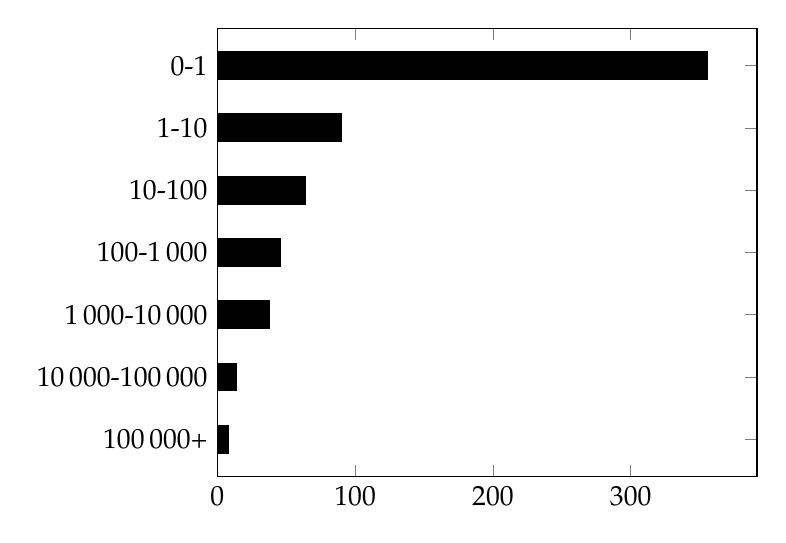
\begin{tikzpicture}
	\pgfplotstableread{
		Balance   			Contracts
		100\,000+			8
		10\,000-100\,000    14
		1\,000-10\,000      38
		100-1\,000      	46
		10-100     			64
		1-10				90
		0-1					356
		%0					3984
	}\datatable
	
	\begin{axis}[
	xbar stacked,   % Stacked horizontal bars
	xmin=0,         % Start x-axis at 0
	ytick=data,     % Use as many tick labels as y coordinates
	yticklabels from table={\datatable}{Balance}
	]
	\addplot [fill=black] table [x=Contracts, y expr=\coordindex] {\datatable};
	\end{axis}
	\end{tikzpicture}
	\caption{Distribution of non-zero contract balances (ether).}
	\label{BalancesFigure}
\end{figure}

The contract balances differ significantly, with most contracts ($3\,984$,~or $86.6\%$) having a zero balance (Figure~\ref{BalancesFigure}).
One contract holds over one~million ether ($1\,500\,000$, or~$440$~million~USD at the time of testing), which accounts for~$38.4\%$~of the total balance of all contracts.
Contracts have from $1$~to $2\,525$~lines of code, with an average of~$334$~lines and a median of~$221$~lines.

\let\letcs\texapiletcs
\begin{figure}
	\centering
	\resizebox{0.8\textwidth}{!}{
	\begin{tikzpicture}[x={(.001,0)}, font=\large]
	\definecolor{darkgray}{RGB}{128,128,128}
	\definecolor{lightgray}{RGB}{232,232,232}
	\foreach  \l/\x/\c[count=\y] in {
		{\usevalue SolidityBytesByte:name }					/{\usevalue SolidityBytesByte:occur }				/lightgray,
		{\usevalue SolidityRedundantFallbackReject:name }	/{\usevalue SolidityRedundantFallbackReject:occur }	/lightgray, 
		{\usevalue SolidityLockedMoney:name }				/{\usevalue SolidityLockedMoney:occur }				/lightgray, 
		{\usevalue SolidityMaliciousLibraries:name }		/{\usevalue SolidityMaliciousLibraries:occur }		/lightgray, 
		{\usevalue SolidityErc20ApiViolation:name }			/{\usevalue SolidityErc20ApiViolation:occur }		/lightgray, 
		{\usevalue SolidityPrivateModifier:name }			/{\usevalue SolidityPrivateModifier:occur }			/lightgray, 
		{\usevalue SolidityStyleGuideViolation:name }		/{\usevalue SolidityStyleGuideViolation:occur }		/lightgray, 
		{\usevalue SolidityIntegerDivision:name }			/{\usevalue SolidityIntegerDivision:occur }			/lightgray, 
		{\usevalue SolidityPragmasVersion:name }			/{\usevalue SolidityPragmasVersion:occur }			/lightgray, 
		%{\usevalue SolidityUncheckedMath:name }			/{\usevalue SolidityUncheckedMath:occur }			/lightgray,
		%{\usevalue SolidityVisibility:name }				/{\usevalue SolidityVisibility:occur }				/lightgray, 
		{\usevalue SolidityBalanceEquality:name }			/{\usevalue SolidityBalanceEquality:occur }		/darkgray,
		{\usevalue SolidityTxOrigin:name }					/{\usevalue SolidityTxOrigin:occur }			/darkgray, 
		{\usevalue SolidityVar:name }						/{\usevalue SolidityVar:occur }					/darkgray,
		{\usevalue SolidityGasLimitAndLoops:name }			/{\usevalue SolidityGasLimitAndLoops:occur }	/darkgray, 
		{\usevalue SoliditySend:name }						/{\usevalue SoliditySend:occur }				/darkgray, 
		{\usevalue SolidityTimestampDependence:name }		/{\usevalue SolidityTimestampDependence:occur }	/darkgray, 
		{\usevalue SolidityDosWithThrow:name }				/{\usevalue SolidityDosWithThrow:occur }		/darkgray,
		{\usevalue SolidityCallValue:name }					/{\usevalue SolidityCallValue:occur }				/black,
		{\usevalue SolidityUncheckedCall:name }				/{\usevalue SolidityUncheckedCall:occur }			/black, 
		{\usevalue SolidityReentrancyExternalCall:name }	/{\usevalue SolidityReentrancyExternalCall:occur }	/black}
	{\node[left] at (0,\y) {\l};
		\fill[\c] (0,\y-.4) rectangle (\x,\y+.4);
		\node[right] at (\x, \y) {\x};}
	\draw (0,0) -- (8000,0);
	\foreach \x in {2000, 4000, ..., 8000}
	{\draw (\x,.3) -- (\x,0) node[below] {\x};}
	\draw (0,0) -- (0,19.4);
	\end{tikzpicture}}	
	\caption{Findings on the big dataset \\ (excluding {\usevalue SolidityVisibility:name }).}
	\label{MassiveTestingFigure}
\end{figure}
\let\letcs\etoolboxletcs

SmartCheck analyzed the dataset in approximately $2$~hours and~$7$~minutes.\footnote{$7\,644$~seconds ($437$~lines per second) on Intel~Core~i5-4210M @ 2.60~GHz, 12~GB RAM, Windows~8.1 64~bit.}
As per SmartCheck, $99.9\%$~of contracts have issues, $63.2\%$~of contracts have critical vulnerabilities\footnote{The issues found by SmartCheck in the big dataset were not manually verified.}.
The findings are presented in Table~\ref{MassiveTestingTable} and Figure~\ref{MassiveTestingFigure} (colors denote severity levels: black -- high, dark gray -- medium, light gray -- low).
The most prevalent issue, \textbf{\let\letcs\texapiletcs \usevalue SolidityVisibility:name \let\letcs\etoolboxletcs} (detected~{\let\letcs\texapiletcs \usevalue SolidityVisibility:occurWord \let\letcs\etoolboxletcs} times, which accounts for $67.30\%$~of all findings), is excluded from the figure for clarity.

\let\letcs\texapiletcs
\begin{table}[t]
	\centering
	\caption{Code issues detected on the big dataset.}
	\begin{tabular}{|c|l|r|r|}
		\hline
		\textbf{Severity} & \textbf{Pattern} & \textbf{Findings} & \textbf{\% of all} \\
		\hline
		\multirow{3}{*}{high} & {\usevalue SolidityReentrancyExternalCall:name } & {\usevalue SolidityReentrancyExternalCall:occurWord } & $3.329$ \\
		 & {\usevalue SolidityUncheckedCall:name } & {\usevalue SolidityUncheckedCall:occurWord } & $0.818$ \\
		 & {\usevalue SolidityCallValue:name } & {\usevalue SolidityCallValue:occurWord } & $0.228$ \\
		\hline
		\multirow{8}{*}{medium} & {\usevalue SolidityDosWithThrow:name } & {\usevalue SolidityDosWithThrow:occurWord } & $6.521$ \\
		& {\usevalue SolidityTimestampDependence:name } & {\usevalue SolidityTimestampDependence:occurWord } & $6.378$ \\
		& {\usevalue SoliditySend:name } & {\usevalue SoliditySend:occurWord } & $2.794$ \\
		& {\usevalue SolidityGasLimitAndLoops:name } & {\usevalue SolidityGasLimitAndLoops:occurWord } & $2.164$ \\
		& {\usevalue SolidityVar:name } & {\usevalue SolidityVar:occurWord } & $0.529$ \\
		& {\usevalue SolidityTxOrigin:name } & {\usevalue SolidityTxOrigin:occurWord } & $0.163$ \\
		& {\usevalue SolidityBalanceEquality:name } & {\usevalue SolidityBalanceEquality:occurWord } & $0.094$ \\
		\hline
		\multirow{10}{*}{low} & {\usevalue SolidityVisibility:name } & {\usevalue SolidityVisibility:occurWord } & $67.296$ \\& {\usevalue SolidityPragmasVersion:name } & {\usevalue SolidityPragmasVersion:occurWord } & $3.067$ \\
		& {\usevalue SolidityIntegerDivision:name } & {\usevalue SolidityIntegerDivision:occurWord } & $1.432$ \\
		& {\usevalue SolidityStyleGuideViolation:name } & {\usevalue SolidityStyleGuideViolation:occurWord } & $1.348$ \\
		& {\usevalue SolidityPrivateModifier:name } & {\usevalue SolidityPrivateModifier:occurWord } & $1.014$ \\
		& {\usevalue SolidityErc20ApiViolation:name } & {\usevalue SolidityErc20ApiViolation:occurWord } & $1.169$ \\
		& {\usevalue SolidityMaliciousLibraries:name } & {\usevalue SolidityMaliciousLibraries:occurWord } & $1.157$ \\
		& {\usevalue SolidityLockedMoney:name } & {\usevalue SolidityLockedMoney:occurWord } & $0.439$ \\
		& {\usevalue SolidityRedundantFallbackReject:name } & {\usevalue SolidityRedundantFallbackReject:occurWord } & $0.053$ \\
		& {\usevalue SolidityBytesByte:name } & {\usevalue SolidityBytesByte:occurWord } & $0.006$ \\
		\hline
	\end{tabular}
	\label{MassiveTestingTable}
\end{table}
\let\letcs\etoolboxletcs


%%%% SECTION 5: RELATED WORK %%%%
% moved to Chapter09

%%%% SECTION 6: CONCLUSION %%%%
\section{Conclusion and future work}
	
We provided a comprehensive overview and classification of code issues in Solidity -- the major high-level language for Ethereum smart contracts.
We implemented SmartCheck -- an efficient static analysis tool for Solidity, which offers significant improvements over existing alternatives.
We tested our tool on a massive set of real-world contracts and detected code issues in most of them.
The tool can be improved in multiple directions: improving the grammar\footnote{The currently used grammar failed to parse $0.16\%$~of lines in our dataset.}, making patterns more precise (e.g.,~the temporarily muted {\usevalue SolidityUncheckedMath:name }), adding new patterns, implementing more sophisticated static analysis methods, adding support for other languages.

Security is still an issue in blockchain development.
We hope that SmartCheck will help solve this major challenge by providing smart contract developers with fast and relevant feedback on potentially problematic source code patterns.

\chapter{Privacy-preserving KYC on Ethereum}

\label{Chapter12KYC}

In this Chapter, we present an Ethereum-based privacy-preserving KYC scheme for token white-listing.\footnote{This Chapter is based on~\cite{Biryukov2018}, which in turn described a hackathon project. A proof-of-concept implementation was created in May~2017 during the Luxblock hackathon in Luxembourg, and was awarded a joint first prize. The team included Daniel Feher, Dmitry Khovratovich, Sergei Tikhomirov, Aleksei Udovenko, and Maciej \.{Z}urad. Contributions of the author of this thesis include: implementing parts of the hackathon project and writing the paper (except for Section~\ref{sec:PrivacyPreservingKYC}).}
We describe the current approach of identity management and propose KYCE -- a privacy-preserving KYC scheme on Ethereum.


%%%%%%%% SECTION 1. Introduction %%%%%%%%

\section{Introduction}

Digital identity is information used by a computer system to represent a user.
Access to services in controlled in two steps:

\begin{itemize}
	\item Authentication: a user proves that they are who they claim to be;
	\item Authorization: the system ensures that the user has the right to perform the requested action.
\end{itemize}

To comply with regulation, financial institutions must verify the identity of their customers.
Modern finance adheres to the centralized identity model and depends on government-issued identities.
Regulation in most jurisdictions demand that banks obtain proof of identity from customers before doing business with them ("know your customer", or KYC).
"Anti money laundering" (AML) and "counter terrorist financing" (CTF) are related regulations that require banks to stop and report suspicious transactions.

Modern KYC practices weaken users' control over their personal information and threats their privacy.
Financial institutions store sensitive information in private databases.
This is a target for corrupt employees or external hackers.
Banks implement KYC/AML procedures independently.
This leads to high compliance cost and multiplies the risk of identity theft.

Blockchain networks like Ethereum aim to serve as a basis of more decentralized identity management.

Open blockchains take a different approach to identity.
Users join these networks without any identification.
This technology enabled the creation of more sophisticated decentralized networks with rich programming capabilities, e.g.,~Ethereum.
Financial service providers establish consortia to apply blockchain technologies in their services~\cite{EEA2017, Hyperledger, R3}.
Though to comply with regulation, they have to handle government-issued identities in a blockchain setting.
This is a non-trivial task, which becomes harder with users' demands for stronger privacy protection.
The European privacy regulation (GDPR~\cite{GDPR16}) that came into force in May~2018 poses more challenges for organizations that handle personal data.

We first explore the centralized and decentralized approaches to identity.
We then propose KYCE -- a privacy preserving Ethereum-based KYC implementation.
KYCE allows banks to implement KYC checks using an external smart contract -- a KYC provider.
Our scheme uses zero-knowledge proofs to check users' eligibility without disclosing their private information to anyone except the KYC provider.
The whitelist is stored in the KYC smart contract in the form of a cryptographic accumulator.
This construction allows users to be efficiently added to, removed from, and checked against a list without storing any plaintext data on the blockchain.
We then discuss possible use cases, implementation challenges, and outline the direction for future work.

\subsection{Centralized identity}

We can re-formulate the notion of identity in terms of asymmetric cryptography.
Identity~$I$ of user~$U$ is a public-private key pair~$(pub_U, priv_U)$.
The public key~$pub_U$ authenticates the user (or, equivalently, links the current action to some past actions).
Public identifiers like username or address are derived from~$pub_U$.
The private key~$priv_U$ allows $U$ to sign messages on behalf of~$I$.
For the system, $U$ is whoever possesses $priv_U$.

In the centralized model of identity, prevalent on the Internet today, users delegate managing their private keys to a trusted party and use a password to access them when necessary.
This approach is sub-optimal in many regards.
First, users do not control their identities.
The trusted party always has the technical ability to sign messages without the user's consent or to prevent the user from signing the message they want.
Moreover, users' personal data is stored by a centralized entity, providing incentives for an attack.
Finally, users have to create a new identity for each website they wish to register with.
As a result, they adhere to a risky practice of reusing passwords.
This problem is partially addressed with the "login with" feature, often implemented using protocols such as OAuth and OpenID~\cite{Dodanduwa2018}.
In this scheme, a third-party website queries the website that holds the user's existing identity (e.g.,~Google) and asks for permission to access a subset of the user's data (e.g.,~name and email).
Upon approval, the access is granted.
This approach alleviates the password management problem but increases the impact of a potential identity theft.

Though users can revoke the access at any time, the "login with" scheme is still privacy violating.
Imagine a user that reveals their date of birth to prove to a website that they are 18 years of age or older.
If they later revoke the access, their date of birth will never change.
Thus, they grant the third-party website effectively unlimited access to a piece of private information.

Maintaining correspondence between "real world" identities and public keys has long been a challenge.
Widely deployed centralized solutions like PKI suffer from risks associated with centralization: a fraudulent authority can issue rogue certificates~\cite{Amann2017}.


\subsection{Decentralized identity and open blockchains}

A noteworthy approach to decentralized identity is the PGP "web of trust"~\cite{Feisthammel2017}.
It has not gained significant traction due in part to usability challenges~\cite{Ruoti2015} and concerns about the security of the long-term key model~\cite{Valsorda2016}.

Bitcoin~\cite{Nakamoto2008} eliminates the problem of connecting public keys to identities in a radical manner: in Bitcoin, public keys \textit{are} identities.
Alternative blockchains such as Ethereum~\cite{Buterin2014, Wood2014} take a similar approach.
%See~\cite{Allen16} on the evolution of identity from centralized to self-sovereign.

%Traditional financial institutions are becoming interested in blockchain technology, especially in networks enabling smart contracts~\cite{Castillo2017}.
The way open blockchains handle identity may come at odds with financial regulation.
We propose a design that will simultaneously leverage the power of blockchain-based smart contracts, enable banks to implement KYC to comply with the law, and preserve users' privacy.


\subsection{Financial and privacy regulation in the EU} \label{sec:Ch12KYCEU}

The current EU legislation "on information accompanying transfers of funds" came into effect in 2015~\cite{EU847}.
In the wake of the rapid growth of cryptocurrencies, the EU is tightening its anti-money laundering regulations, stating that "virtual currency exchange platforms and custodian wallet providers will have to apply customer due diligence controls, ending the anonymity associated with such exchanges"~\cite{EU16}.
See~\cite{Vandezande2017} for an analysis of virtual currencies under the EU anti-money laundering law.

In 2018, two pieces of legislation came into force in the EU.

\begin{itemize}
	\item The \textbf{Revised Payment Service Directive} (PSD2) obligates banks to provide access to their customers' accounts through open APIs~\cite{Hellstroem2017}.
	This measure is meant to foster competition and give rise to third-party financial service providers.
	For instance, unified banking API will likely simplify connecting banking infrastructure to open blockchains~\cite{Elison2016}.
	\item The \textbf{General Data Protection Regulation} (GDPR), coming into force on 25~May~2018, harmonizes data privacy laws across the EU~\cite{GDPR16} and introduces stricter rules for handling data of EU residents even for companies from outside the EU. We refer the reader to~\cite{Berberich2016} describes possible implications of blockchain adoption from the viewpoint of the EU data protection regulation.
\end{itemize}



%%%%%%%% SECTION 2. KYCE %%%%%%%%

\section{KYCE: a decentralized KYC-compliant exchange}

KYC requirements differ depending on jurisdiction~\cite{PWC2015}.
A typical KYC procedure links users' real-world identities to their accounts and checks users against a whitelist or a blacklist.
The details of the KYC procedure do not affect our design.

\subsection{Definitions and security properties}

\begin{definition}
	A \textbf{KYC procedure} is a process that determines if a given user is eligible for a given transaction.
\end{definition}

\begin{definition}
	A \textbf{KYC provider} is an entity that performs a KYC procedure.
\end{definition}

\begin{definition}
	A \textbf{financial service} is an information system that allows users to exchange units of value.
\end{definition}

\begin{definition}
	A financial service is \textbf{KYC-compliant} w.r.t.~the KYC procedure if and only if all users are eligible for all transactions they perform.
\end{definition}

\begin{definition}
	A KYC-compliant financial service is \textbf{privacy-preserving} if and only if only the KYC provider has access to the users' private data.
\end{definition}


\subsection{Tokens and exchanges}

Our KYC solution can be applied for any service.
For concreteness, consider a token exchange as an example of a financial service.

\begin{definition}
	A \textbf{token} is a transferable fungible unit of value maintained by a smart contract.
\end{definition}

ERC20~\cite{Victor2019} is the de-facto standard API for implementing token contracts in Ethereum.
A token contract keeps track of users' token balances and enables them to transfer tokens using the following functions:

\begin{itemize}
	\item \texttt{transfer} sends a given amount of tokens to a given address.
	\item \texttt{approve} allows a given user to withdraw up to a given amount of tokens from the account of the user calling the function.
	\item \texttt{transferFrom} sends a given amount of tokens from one given address to another (the amount has to be \texttt{approve}d beforehand).
\end{itemize}

\begin{definition}
	An \textbf{exchange} is a service that enables users to exchange tokens.
\end{definition}

Centralized exchanges, implemented as a regular web service, are the most prevalent.
In this work, we are mostly interested in decentralized, or on-chain exchanges, implemented as smart contracts. 

An exchange without KYC support may be used as follows.
\begin{enumerate}
	\item Alice creates an order to sell $X$~A-tokens for $Y$~B-tokens.
	\item Bob creates an order to sell $Y$~B-tokens for $X$~A-tokens.
	\item The exchange matches the two orders and transfers (by calling \texttt{transferFrom}) $X$~A-tokens from Alice to Bob and~$Y$~B-tokens from Bob to Alice.
\end{enumerate}

The transaction succeeds if Alice and Bob \texttt{approve}d the exchange with sufficient amount of A- and B-tokens respectively before \texttt{transferFrom} is called.
Users withdraw tokens from the exchange by calling \texttt{approve(exchangeAddress,0)}.



\subsection{Privacy-preserving KYC}
\label{sec:PrivacyPreservingKYC}

We propose KYCE -- a privacy-preserving KYC design for Ethereum-based financial services.

A KYC contract provides an API to other contracts so that external services can determine if a given user is KYC-approved for using a given token.
A KYC provider (a governmental entity or company in charge of customer onboarding) performs the necessary checks for a new customer and adds their address to the whitelist.

A simple approach to implementing KYC check with a separate contract would be the following.
The KYC contract stores the whitelist of approved addresses.
On every \texttt{transfer}, token contracts check if the address belongs to the whitelist.
This design has a fundamental privacy flaw: all whitelisted addresses are stored on the blockchain in plaintext.
Moreover, users must use the same addresses they registered with the KYC provider.
This also threatens privacy: an adversary can link the user's transactions using public blockchain data.

\paragraph{Our approach}
We use cryptographic techniques to design a privacy preserving KYC solution.
In KYCE, the KYC contract stores a \textbf{cryptographic accumulator} of the whitelisted addresses. 

A cryptographic accumulator~$A$ absorbs certain algebraic objects and provides an interface to generate and verify zero-knowledge proofs that a given value was accumulated.
In our construction, to generate a proof for value~$x\in A$, one needs a \textit{witness} that depends on~$A$ and~$x$.
The accumulator owner provides the witness to the user who submitted $x$.
We suggest an accumulator based on bilinear maps~\cite{Camenisch2009}.

The KYC setup and workflow is as follows.
The KYC provider publishes a smart contract and initializes it with an empty accumulator.
The User interacts with the KYC provider physically or online and provides the credentials needed to pass the verification.
The User also generates their own master secret~$m$ and during the authenticated session gives the provider a Pedersen commitment~$g_1^m\cdot g_2^r$ to it.
$g_1$ and~$g_2$ are certain group generators\footnote{Here and in the further text all multiplications take place in the pre-selected group of prime order~$q$, typically an elliptic-curve group.}, and~$r$ is random.
If the checks are passed, the provider updates the accumulator with user-dependent data and provides the User with a witness.
In every subsequent Ethereum transaction to KYCE, the User provides a proof that they have been registered in the accumulator, that this right has not been revoked, and that the proof owner and the transaction sender are the same person.
KYCE verifies the last statement.
The KYC contract verifies the rest against the current accumulator value.
If the checks pass, the requested action is executed in KYCE.

\paragraph{Details on the accumulator construction}
We construct an accumulator based on a pairing function~$e(\cdot,\cdot)$ in some pairing setting.\footnote{The original paper~\cite{Camenisch2009} uses type-1 pairings, but type-3 pairings can be adopted as well.}.
The accumulator contains the serial numbers, possibly consecutive integers.\footnote{It is possible to store public keys but it would be less efficient.}

The accumulator is constructed as follows.
We assume a bilinear pairing~$e:\,G\times G\rightarrow G_T$, where $G,G_T$ are groups of order~$q$.
The KYC provider selects a generator~$g$ and a secret value $\gamma\overset{\$}{\leftarrow} \mathbb{Z}_q$.
It also selects $L$ as an upper bound of users enabled for KYC and computes $z = e(g,g)^{\gamma^{L+1}}$.
It initialized the accumulator value~$\mathrm{A}$ by $1$. 

Let us denote $g_i = g^{\gamma^i}$.
The provider publishes $\mathrm{A},\{g_i\}_{1\leq i\leq L, \,L+2\leq i \leq 2L}$, the set of registered KYC indices $V=\emptyset$, and the parameters $g,z$ needed for verification.

Every User who passes the KYC check is issued a new serial number~$i$, the witness~$w_i = \prod_{j\in V,j\neq i} g_{L+1-j+i}$, where $V$ is the set of all issued serial numbers, and a signature~$\sigma_i$ of~$g_i||i$ on the provider's private signature key.
The witness is used to generate a proof of accumulating.\footnote{We refer an interested reader to~\cite{Camenisch2009} for the details.}
The accumulator is updated by the KYC provider with~$i$ by
$$
\mathrm{A_{V\cup\{i\}}} \leftarrow \mathrm{A_V} \cdot g_{L+1-i}
$$
multiplying it by $g_{L+1-i} = g^{\gamma^{L+1-i}}$, and~$i$ is published as a new valid serial number.
To prove that $i$ has been committed to $A$ and has not been revoked without disclosing it, the holder of~$w_i$ updates it\footnote{We omit the details, but the update can be performed just before the presentation, not necessarily after every accumulator update.} so that the following equation holds:
$$
\frac{e(g_i, A)}{e(g,w_i)} = z.
$$

Note that revocation is also efficient.
The KYC contract owner simply multiplies the accumulator value by the inverse of~$g_{L+1-i}$.
The witness value can not be updated anymore.

\paragraph{Presentation} 
When issuing a transaction to use the exchange (e.g.,~create an order), the user submits a \textbf{zero-knowledge proof} of the following statement:
\begin{itemize}
	\item I know the private key of the current user address (\texttt{msg.sender}), and
	\item I know a signature~$\sigma_i$ and a witness~$w_i$ for some number~$i$ that has been accumulated in the
	accumulator~$A$ in the KYC contract.
\end{itemize}
It is crucial that this compound statement is \textit{atomic}, i.e.,~the sub-statements can not be extracted as separate valid proofs, as this would make the transaction malleable.

The atomicity (and non-malleability) are ensured as follows.
Let us denote the proof of knowledge for the witness and signature by~$PK_w$.
Then the Prover submits 
$$
P = \{PK_w \wedge PK_s\},
$$
where $PK_s$ is the proof of knowledge of the private key of the \texttt{msg.sender}'s ECDSA public key, which can be taken from~\cite{Chase2016}.
The technique to make a composite proof of knowledge (PoK) is straightforward, as both PoKs are non-interactive, and is standard in complex PoK protocols:
\begin{enumerate}
	\item The Prover collects a set $\mathcal{C}$ of commitments asserted in sub-proofs $PK_w$ and~$PK_s$.
	\item The Prover makes necessary randomization of~$\mathcal{C}$ to create $t$-values $\mathcal{T}$.
	\item The Prover computes $c \leftarrow H(\mathcal{C},\mathcal{T})$.
	\item The Prover computes $s$-values $\mathcal{S}$ using
	$\mathcal{C}$, $\mathcal{T}$, and~$c$.
	\item The proof~$P$ is $(\mathcal{C}, \mathcal{S},c)$.
	To verify it one computes asserted $t$-values $\widehat{\mathcal{T}}$ and verifies
	$$
	c\overset{?}{=}H(\mathcal{C},\widehat{\mathcal{T}}).
	$$
\end{enumerate}

The resulting proof~$P$ is submitted as an Ethereum transaction argument.
KYCE retrieves the most recent accumulator value and verifies $P$ against it and the public key of the message sender, available in the transaction metadata.
If the proof is correct, the order is executed.


\subsection{Use cases}

Either the exchange contract or the token contract must be KYC-compliant -- i.e.,~check eligibility of transacting parties using the implementation of the introduced cryptographic scheme using the KYC contract.

\paragraph{KYC-compliant exchange}

If the exchange is KYC-compliant, the tokens do not need to be aware of the KYC (Figure~\ref{fig:KYCCompliantExchange}).

\begin{figure}[h]
	\centering
	\includegraphics[width=0.8\textwidth]{figure-kyc-exchange}
	\caption{KYC-compliant exchange.}
	\label{fig:KYCCompliantExchange}
\end{figure}

Consider an established exchange that trades dozens of tokens.
It applies for official approval in a jurisdiction that requires all customers to pass the KYC procedure.
The governmental body acts as a KYC provider, deploys a KYC contract, and publishes its address.
The exchange adds KYC checks to its codebase and continues operation.
Users who do not want to apply for KYC can withdraw their tokens from the exchange.


\paragraph{KYC-compliant token}

If the token is KYC-compliant, the exchange does not need to be aware of the KYC (Figure~\ref{fig:KYCCompliantToken}).

\begin{figure}[h]
	\centering
	\includegraphics[width=0.8\textwidth]{figure-kyc-token}
	\caption{KYC-compliant token.}
	\label{fig:KYCCompliantToken}
\end{figure}

Consider a government that issues its own tokens.\footnote{Bank of England~\cite{Danezis2016} and the Monetary Authority of Singapore~\cite{Singapore17} already did research in this direction.}
Government tokens could be used by KYC-approved users for tax payments, fees, and fines.
Such solution leverages the flexibility and auditability of smart contracts while only allowing approved entities to use the token.
The KYC-enabled government token can be also traded on exchanges.
This allows citizens to hold their wealth in currency portfolios of their choice and only purchase government tokens to transact with the state.

\paragraph{Transaction-dependent checks}

Many jurisdictions impose restrictions that depend on the value of the transaction.
E.g.,~the EU regulation~\cite{EU847} states that "the obligation to check whether information on the payer or the payee is accurate should \textelp{} be imposed only in respect of individual transfers of funds that exceed \EUR{1\,000}".
EU member states impose further restrictions for large transactions, e.g.,~exceeding \EUR{10\,000} in Belgium, \EUR{15\,000} in Germany and in the Netherlands~\cite{PWC2015}.
Either the exchange contract or the token contract can perform such checks by storing the following mappings:
\begin{itemize}
	\item address $=>$ accumulated transaction volume in the current period (day, month, year);
	\item address $=>$ timestamp of the latest transaction. 
\end{itemize}



%%%%%%%% SECTION 3. Implementation details %%%%%%%%

\section{Implementation details}

We created an initial (not privacy-preserving) implementation of the proposed design.
Our project consists of two smart contracts written in Solidity: KycProvider and KyceToken.
KycProvider maintains a 2-dimensional boolean array that stores the eligibility status across users and tokens.
On initialization, the address that deploys the contract to the blockchain is made the \textit{owner}, allowing it to add and remove users from the array.
The ownership may be transferred (using the functionality inherited from the standard \texttt{Ownable} contract).

The KycProvider exposes the following API:

\begin{itemize}
	\item \texttt{add(address \_user, address \_token)} makes the user eligible for using the token (callable only by the owner);
	\item \texttt{remove(address \_user, address \_token)} makes the user not eligible for using the token (callable only by the owner);
	\item \texttt{isEligible(address \_user, address \_token)} checks if the user is eligible for using the token.
\end{itemize}

KyceToken adheres to the de-facto standard token API in Ethereum -- ERC20.
To minimize the risk of security issues due to implementation subtleties, we inherit a widely used and tested ERC20 implementation by OpenZeppelin.
We override the functions \texttt{approve}, \texttt{transfer}, and \texttt{transferFrom} to check if the given user (\texttt{msg.sender}) is eligible for using this token.
If \texttt{isEligible} returns \texttt{false}, the execution stops.
If it returns \texttt{true}, the corresponding function of the super class is invoked.

The implementation of the proposed scheme requires certain cryptographic primitives.
Some of them are already partially available in Ethereum as pre-compiled contracts (namely, elliptic curve addition, scalar multiplication, and pairing checks).
For the proposed scheme to be fully implemented, pairing evaluation is also required.\footnote{As of 2020, Ethereum does not support pairing evaluation.}
%We are looking into the possibilities to add this functionality.


%%%%%%%% SECTION 4. Related work %%%%%%%%

\section{Related work}

Parra-Moyano and Ross use distributed ledger technology to improve the KYC process~\cite{Moyano2017}.
Their proposal can be summarized as follows:
\begin{itemize}
	\item the regulator maintains a database with all users' private data;
	\item the users signs a contract with their first bank (the\textit{home bank});
	\item the home bank stores hashes of the user's documents in a smart contract in a permissioned blockchain;
	\item when a user signs a contract with another bank it obtains the user's documents from the database and looks up the hash to ensure that the user had been KYC-approved;
	\item the identity of the home bank is not revealed;
	\item a cost-sharing mechanism for banks allows to proportionally share the cost of the initial KYC approval.
\end{itemize}
In this design, all banks store users' private data -- contrary to our solution, where it is stored only with the KYC provider.
A more decentralized design is also proposed, but the authors claim it to be of a lesser practical relevance.

Sullivan and Burger investigate possible implications of further development of the Estonian e-residency program using blockchain technology~\cite{Sullivan2017}.
E-residency of Estonia is a governmental program that provides applicants with a digital identity that can be used, e.g.,~to register a company and open a bank account.
Estonian e-residency disconnects a digital identity from citizenship or physical residence.
Within the e-residency program, Estonia collaborates with a blockchain project Bitnation~\cite{Bitnation15, Estonia15}.
Provable (previously known as Oraclize) implemented a connector that lets Ethereum contracts handle e-residency identities~\cite{Provable}.

A project~\cite{Ohtamaa2016} similar to ours implements a KYC scheme in an Ethereum smart contract, but stores the KYC status on the blockchain in plaintext.
Multiple projects aim at easing customer onboarding for banks~\cite{CambridgeBlockchain, KycChain, SnapSwap, Tradle}.
Blockchain consortium R3 developed a proof-of-concept implementation of a shared KYC between ten banks based on its blockchain platform Corda~\cite{Allison2016}.
Multiple Ethereum-based identity projects have been proposed~\cite{Mesropyan2017, Sovrin, Uport}.


%%%%%%%% SECTION 5. Conclusion and future work %%%%%%%%

\section{Conclusion}

We proposed a modular design of an Ethereum-based financial service with an external KYC check, which brings benefits to all participants:

\begin{itemize}
	\item \textbf{Users} obtain a unified identity that they can use with multiple financial services.
	Users' personal data is stored only with the KYC provider and can be easily updated.
	Personal data is neither stored on the blockchain nor transmitted to third parties.
	\item \textbf{Financial services} greatly simplify the KYC process: it boils down to a single API call.
	Our design lets them cut KYC costs while at the same time diminishing risks of handling sensitive data.
	\item \textbf{Governments} get an opportunity to stimulate innovation in the financial sector by providing a unified and simple KYC API\@.
	This is especially relevant in the context of rapidly growing fintech and blockchain industries.
\end{itemize}

Our design is agnostic to the nature of the entity behind the KYC contract.
It does not have to be a government body.
The proposed solution can be used in any setting where a smart contract based service wants to limit the set of its users.
For instance, many jurisdictions (e.g.,~the~US~\cite{SEC}) only allow certain investments to be offered to "accredited investors".
These are typically high-net-worth individuals and financial institutions.
This logic can be replicated in a blockchain setting.
Consider a blockchain-based financial service that only accepts cryptocurrency users who possess more than $10\,000$~USD and did their first transaction before~2017.
The "accrediting" functionality is delegated to a third party KYC provider.
Proving net worth and previous activity on the blockchain is straightforward.
More checks can be added.
Once accredited, an investor can use multiple "restricted" services without revealing any personal details to their developers.



%\bookmarksetupnext{level=chapter}
%\chapter{Conclusion}

\label{Chapter13Conclusion}

We summarize the thesis and present an outlook into the future of blockchains, cryptocurrencies, and money in general.

\section{Future directions}

\subsection{Improving P2P privacy in cryptocurrencies}

Cryptocurrency developers should introduce privacy enhancing measures at the network level, especially if the currency is meant to be privacy-preserving.
As our results show, trickling and diffusion, as they are implemented in Bitcoin and its forks, are not sufficient.

\paragraph{Better P2P propagation in Bitcon}
As we have outlines, Dandelion~\cite{Venkatakrishnan2017, Fanti2018} may be a promising way to improve the privacy of Bitcoin and other cryptocurrencies on the networking level.
Dandelion has already been implemented and is currently used in a privacy-focused cryptocurrency Grin.
Its use, however, has been shown to have weaknesses.
\todo[inline]{Discuss what Dandelion does and doesn't; ref Bogatyy's post}

\subsubsection*{Improving our clustering technique}

\paragraph{The applicability of the external quality metric}
The adjusted anonymity degree, which we used as an external quality metric, has limitations.
In particular, we didn't account for transactions from clusters which did not also contain at least one of our own transactions.
The rationale behind this is the lack of the ground truth for two "foreign" transactions: we do not know whether they should be included in the same cluster.
Consequently, our quality metric may poorly reflect the reality on large networks (such as the Bitcoin mainnet), where our transactions make up only a small part of the full network throughput.
One direction of future research may be deriving an anonymity metric which works better under these circumstances.

\paragraph{Direct comparison of relay randomization techniques}
As described in Section~\ref{sec:Ch03Background}, cryptocurrencies use different relay randomization techniques aimed at improving privacy: trickling, diffusion, or no randomization.
A natural question would be to measure the relative effectiveness of these methods.
Unfortunately, we cannot use a direct comparison between cryptocurrencies that use diffusion and trickling to make a conclusion about relative effectiveness of these methods, as the real-world networks also differ in many other parameters (such as the number of nodes and transaction rate) that also influence the attack results.
A possible direction for future research may be to quantify the effects of trickling and diffusion on privacy properties of a Bitcoin-like cryptocurrency with respect to our attack technique, holding all other parameters equal.

%----------------------------------------------------------------------------------------
%	THESIS CONTENT - APPENDICES
%----------------------------------------------------------------------------------------

\appendix % Cue to tell LaTeX that the following "chapters" are Appendices

% Include the appendices of the thesis as separate files from the Appendices folder
% Uncomment the lines as you write the Appendices

%\include{Appendices/AppendixA}
%\include{Appendices/AppendixB}
%\include{Appendices/AppendixC}

%----------------------------------------------------------------------------------------
%	BIBLIOGRAPHY
%----------------------------------------------------------------------------------------

\printbibliography[heading=bibintoc]

\setcounter{secnumdepth}{-1}
\chapter*{List of Publications}
\label{sec:ListOfPublications}
\addcontentsline{toc}{section}{\nameref{sec:ListOfPublications}}

\begin{enumerate}
	\item \fullcite{Biryukov2017} (\cite{Biryukov2017})
	\item \fullcite{Tikhomirov2017} (\cite{Tikhomirov2017})
	\item \fullcite{Biryukov2018} (\cite{Biryukov2018})
	\item \fullcite{Tikhomirov2018} (\cite{Tikhomirov2018})
	\item \fullcite{Biryukov2019b} (\cite{Biryukov2019b})
	\item \fullcite{Biryukov2019a} (\cite{Biryukov2019a})
	\item \fullcite{Biryukov2019} (\cite{Biryukov2019})
	\item \fullcite{Tikhomirov2020a} (\cite{Tikhomirov2020a})
	\item \fullcite{Tikhomirov2020} (\cite{Tikhomirov2020})
\end{enumerate}
%----------------------------------------------------------------------------------------

\end{document}  
